%%%%%%%%%%%%%%%%%%%%%%%%%%%%%%%%%%%%%%%%%%%%%%%%%%%%%%%%%%%%%%%%%%%%%%%%
%                                                                      %
% LaTeX, FIIW thesis template                                          %
%                                                                      %
%%%%%%%%%%%%%%%%%%%%%%%%%%%%%%%%%%%%%%%%%%%%%%%%%%%%%%%%%%%%%%%%%%%%%%%%
%\documentclass[11pt,a4paper]{report}
% Indien je je thesis recto-verso wil afdrukken gebruik je onderstaande opties i.p.v. bovenstaande
\documentclass[11pt,a4paper,twoside,openright]{report}

\usepackage[a4paper,left=3.5cm, right=2.5cm, top=3.5cm, bottom=3.5cm]{geometry}
\usepackage[english]{babel}
\usepackage{graphicx}
\usepackage[latin1]{inputenc}           % om niet ascii karakters rechtstreeks te kunnen inputten
%\usepackage[utf8]{inputenc}            % commentarieer deze regel uit als je utf8 encoded files gebruikt in plaats van latin1
\usepackage{natbib}
\usepackage{listings}             		% voor het weergeven van broncode
\usepackage{verbatim}					% weergeven van code, commando's, ...
\usepackage{hyperref}					% maak PDF van de thesis navigeerbaar
\usepackage{varioref}
\usepackage{url}						% URL's invoegen in tekst met behulp van \url{http://}
\usepackage[small,bf,hang]{caption}     % om de captions wat te verbeteren
\usepackage[final]{pdfpages}            % gebruikt voor het invoegen van het artikel in pdf-formaat
\usepackage{pslatex}					% andere lettertype's dan de standaard types
\usepackage{lipsum}
\usepackage{sectsty}					% aanpassen van de fonts van sections en chapters
\usepackage{mathrsfs}					% mathematical variables in a certain fond
\usepackage[]{algorithm2e}				% to write pseudo code
%\usepackage[nottoc,numbib]{tocbibind}	% Bibliography mee in de ToC

\allsectionsfont{\sffamily}
\chapterfont{\raggedleft\sffamily}

\usepackage{float}                      % De optie H voor de plaatsing van figuren op de plaats waar je ze invoegt. bvb. \begin{figure}[H]
%\usepackage{longtable}					% tabellen die over meerdere pagina's gespreid worden
%\usepackage[times]{quotchap}           % indien je fancy hoofdstuktitels wil
%\usepackage[none]{hyphenat}
%\usepackage{latexsym}
\usepackage{amsmath}
\usepackage{amssymb}
\usepackage{longtable}

% MFA: zet zoekpad voor figure
\graphicspath{{fig/}}

\usepackage{fiiw}
\usepackage{fiiw_eng} % For the english version (also change last page at the bottom of this file!

%door onderstaande regels in commentaar te zetten, of op false, kan je pagina's weglaten
%bijvoorbeeld het weglaten van een voorwoord, lijst met symbolen, ...
%%%%%%%%%%%%%%%%%%%%%%%%%%%%%%%%%%%%%%%%%%%%%%%%%%%%%%%%%%%%%%%%%%%%%%%%%%%%%%%%%%%%%%%%
%voorwoord toevoegen?
\acknowledgementspagetrue
\acknowledgements{voorwoord}			%.tex file met daarin het voorwoord

%samenvatting toevoegen
\summarypagetrue
\summary{samenvatting}					%.tex met daarin de samenvatting

%abstract toevoegen?
\abstractpagetrue
\abstracts{abstract}					%.tex file met daarin het abstract
%lijst van figuren toevoegen?
\listoffigurespagetrue
%lijst van tabellen toevoegen?
\listoftablespagetrue
%lijst van symbolen toevoegen?
\listofsymbolspagetrue
\listofsymbols{symbolen}				%.tex file met daarin de lijst van symbolen
%lijst van afkortingen toevoegen?
\listofabbrevspagetrue
\listofabbrevs{afkortingen}				%.tex file met daarin de lijst van afkortingen

%informatie over het eindwerk, de promotor, ...
%%%%%%%%%%%%%%%%%%%%%%%%%%%%%%%%%%%%%%%%%%%%%%%
\opleiding{Industrial Engineering }
\afdeling{Electronics and ICT: Software}

\campus{gent} %denayer,denayereng,geel,geeleng,gent,ghenteng,groept,groupteng,brugge,brugeseng

% onder embargo? laat leeg indien van niet; vul de datum in als dd-mm-yyyy indien van wel
\embargo{}

\title{Measuring HPC Performance of the Parallel FS LS-SVM Algorithm }
\subtitle{}
% \author{naam student}
\forenameA{Pelle}
\surnameA{Reyniers}

% l
\forenameB{}
\surnameB{}

\academicyear{2019 - 2020}

\promotorA[Promotor(en)]{Prof. dr. ir. Wauters T}
\promotorB[Co-promotor(en)]{Prof. dr. ir. De Brabanter J }
\promotorC[]{}

\begin{document}
%\selectlanguage{dutch}
\selectlanguage{english} % For the english version
\preface
%\chapter*{List of Abbreviations}
\addcontentsline{toc}{chapter}{List of Abbreviations}
All abbreviations used in the text.
\begin{longtable}{ll}
	ALU       & Arithmetic Logic Unit                                      \\
	AMD       & Advanced Micro Devices                                     \\
	API       & Application Programming Interface                          \\
	ARM       & original: Acorn RISC Machine, today: Advanced RISC Machine \\
	AWS		  & Amazon Web Services										   \\
	CCE       & Cray Compilation Environment                               \\
	CPU       & Central Processing Unit                                    \\
	CSA       & Coupled Simulated Annealing                                \\
	CSA-BA    & Coupled Simulated Annealing Blind Approach                 \\
	CSA-M     & Coupled Simulated Annealing Modified                       \\
	CSA-MuSA  & Coupled Simulated Annealing Multi State                    \\
	CSA-MwVC  & Coupled Simulated Annealing Modified with Variance Control \\
	CU        & Control Unit                                               \\
	cuBLAS    & CUDA Basic Linear Algebra Subprograms                      \\
	CUDA      & Compute Unified Device Architecture                        \\
	cuDNN     & CUDA                                                       \\
	cuFFT     & CUDA Fast Fourier Transform                                \\
	cuRAND    & CUDA Randomizer                                            \\
	cuSOLVER  & CUDA Solver                                                \\
	cuSPARSE  & CUDA Sparse                                                \\
	DS        & Data Stream                                                \\
	FS LS-SVM & Fixed Size Least Square Support Vector Machines            \\
	GCC       & GNU Compiler Collection                                    \\
	GPU       & Graphical Processing Unit                                  \\
	GRE       & GPU Rest Engine                                            \\
	HDFS      & High Dimensional Feature Space                             \\
	HPC       & High Performance Computing                                 \\
	IO        & Input/Output                                               \\
	IS        & Instruction Stream                                         \\
	KKT       & Karush Kuhn Tucker                                         \\
	LM        & Local Memory                                               \\
	LS-SVM    & Least Square Support Vector Machines                       \\
	MIMD      & Multiple Instruction Multiple Datastream                   \\
	OpenMP    & Open Multi Processing                                      \\
	NPP       & NVIDIA 2D Image And Signal Performance Primitives          \\
	OS        & Operating System                                           \\
	PGI       & Premiere Global Services, Inc.                             \\
	PU        & Processing Unit                                            \\
	RBF       & Radial Base Function                                       \\
	SA        & Simulated Annealing                                        \\
	SIMD      & Single Instruction Multiple Datastream                     \\
	SMP       & Symmetric Multi Processor Organozations                    \\
	SV        & Support Vector(s)                                          \\
	SVM       & Support Vector Machines               
\end{longtable}


%%%%%%%%%%%%%%%%%%%%%%%%%%%%%%%%%%%%%%%%%%%%%%%%%%%%%%%%%%%%%%%%%%% 
%                                                                 %
%                            CHAPTER                              %
%                                                                 %
%%%%%%%%%%%%%%%%%%%%%%%%%%%%%%%%%%%%%%%%%%%%%%%%%%%%%%%%%%%%%%%%%%% 

\chapter{Introduction}
\section{History and Scope}
The rise of machine learning is unmistakable connected to the development of other scientific branches.
First of is the development of computer systems.  
Designing computer systems originated out of the need to do more and more difficult calculations, most desirable with a far larger speed than the human brain ever could.
A pioneer definitely worth mentioning is Alan Turing who built the enigma machine in the 1940's.
Enigma was the name of the code that the Germans used to encrypt their transmissions in the second world war.
His enigma machine is often referred to as one of the first real computers, it was designed and used to crack this German enigma code.
\par
In a parallel timeline Donald Hebb is responsible for creating an abstract model of a brain cell, or neuron.\cite{HebbDonaldOlding1949Wiley}
In his book D. Hebb explains the functioning of a neuron and translates this to more abstract models complete with mathematical representations.
\par 
In the 1950s Arthur Samuel developed a computer program to play checkers with as an objective calculate the move that gives the best winning opportunities.\cite{McCarthy_Feigenbaum_1990} 
In this program Samuel pioneered concepts that stick around to this day.
The fact that computer systems at the time do not have a lot of memory available, forced A. Samuel to invent a, later to be, very important algorithm: \textit{alpha-beta pruning}.
In \textit{alpha-beta pruning} every situation on a board is called a state.
The algorithm makes decisions based on scores it presents to every state, those scores are calculated based on winning probability. 
By sorting possible states in three form, and not analysing branches of the threes that are never going to be possible.
This algorithm is good in generating the best possible move with having a competitive memory and computational complexity.
\par 
All those developments throughout the first half of the 20th century, together with the rise of optimization, heuristics, meta-heuristics and early concepts of Artificial Intelligence, created a fertile environment for the birth of real \textit{Machine Learning} algorithms and principles.
\par
Nowadays, a variety of \textit{Machine Learning} algorithms are available, dividable into different categories.
Regression, Instance-based, Regularization, SVMs, Decision Tree, Bayesian, Clustering, Association Rule Learning, Artificial Neural Network, Deep Learning, Dimensionality Reduction, etc.
A common characteristic of the algorithms throughout the different categories is the computational need, mostly in the form of vector and matrix transformations/calculations.
This explains the rising popularity as computational power in computer systems grew.
\par 
In recent years and decades parallel computing became more accessible thanks to a number of tools and languages that provide better support for developers who have the need to write their programs for parallel execution.
On the hardware side we see the following facts:  most to all of modern CPU's support multi threading and the development of CUDA by NVIDIA, which made it much more accessible to directly use the GPU, and also the more common availability of clusters and supercomputers.
The combination of those elements together with the need to a large number of linear algebraic computations,
create an environment where parallelization is very attractive.
\section{Objectives}
The main objective of this research is to study the behaviour of the FS LS-SVM algorithm in High Performance Computing environments. 
More into detail the following objectives can be stated related to the complete research project:
\begin{itemize}
	\item To make a study of the Fixed Size Least Square Support Vector Machines algorithm.
	\item To get a general understanding of all the elements of the Fixed Size Least Square Support Vector Machines algorithm.
	\item To make a study of the possibilities for parallel programming and code execution as well as HPC environments.
	\item To construct an analysis to predict which parts of the FS LS-SVM are good candidates for parallel execution.
	\item To construct a model in a programming language capable of both sequential and parallel execution, while making remote execution on an HPC environment possible.
	\item To construct tests to describe the behaviour of the model.
	\item To test the algorithm for function estimation and binary classification with data sets containing at least 500 000 data points and 50 attributes.
\end{itemize}
\section{Outline}
In chapter 2, an extensive literature review is given. 
Covering the background of all the elements used in this research, starting with Machine Learning and narrowing down to Support Vector machines, Least Square Support Vector Machines and Fixed Size Least Square Support Vector Machines. After that jumping out of the machine learning and into the world of computing, parallel computing and High Performance Computing.\\
Chapter 3 is a description of the research process, this is in my opinion necessary because it helps to justify why certain decisions are taken in the process.\\
Chapter 4 is a detailed analysis of all the elements of the FS LS-SVM algorithm and their capability to be executed in parallel.\\
Chapter 5 describes the test that are done. For every test, a detailed description is given as well as an hypothesis and result reflection.\\
In chapter 6, a general conclusion corresponding to the tests and the research is formulated.\\
A look at the future and ideas of follow up research are described in chapter 7.
%%%%%%%%%%%%%%%%%%%%%%%%%%%%%%%%%%%%%%%%%%%%%%%%%%%%%%%%%%%%%%%%%%% 
%                                                                 %
%                            CHAPTER 2                            %
%                                                                 %
%%%%%%%%%%%%%%%%%%%%%%%%%%%%%%%%%%%%%%%%%%%%%%%%%%%%%%%%%%%%%%%%%%% 

\chapter{Literature Review}

\section{Introduction}
Understanding the \textit{LS-SVM} algorithm requires a background knowledge spread out over multiple fields.
A good and firm understanding is needed to see the full potential of the algorithm as well as being able to identify the opportunities and challenges corresponding to the parallelization of the algorithm.
Therefore studies in \textit{Machine Learning}, \textit{Optimization}, \textit{Parallel Computing} and \textit{Linear Algebra} are recommended.
 
\section{Machine Learning}
Machine learning, it is a title that gives a somewhat mythical idea to a lot of people.
Where in the early stages research and articles were always written inside the computer science or mathematical engineering community, 
nowadays we can notice that \textit{Machine Learning} algorithms are widespread used to tackle problems in fields far outside computer science.
From economic over biology up to social sciences.
In all fields where data sets of a certain kind are available to learn from, \textit{Machine Learning} algorithms may offer solutions.

\subsection{Introduction}
\textit{Machine Learning} is a sub category of the  \textit{Artificial Intelligence} family.
It is a prime example where the clue is in the name.
The field of machine learning covers algorithms and mathematics used by computers (machines) to identify and learn things based on available data.
This first definition is probably as vague as the title itself for most people.
Learning for a machine/computer has everything to do with making decisions. 
It is smart decision making, based on available data and not based on hard coded rules.
Not being based on hard coded rules comes with some advantages.
It brings a form of flexibility and dynamics to decision software. 
The next paragraph provides an example describing one kind of \textit{Machine Learning}.
\par
Imagine a spam filter who has to make a decision about incoming emails, as shown in figure~\ref{fig:spamham}.
This decision is defined very easily: is the incoming email spam or ham?
In the field of \textit{Machine Learning} this kind of problem is called a classification.
Every email is considered a data entry into the system, with this philosophy the decision question can be rewritten as: does this data entry belong to the previously stated category or not.
In a classic, non \textit{Machine Learning} way, an option is to hard code rules.
The system would use those rules to determine if the data entry is in fact spam.
A system with a design like this would require a heavy lot of maintenance because of the following reasons.
All the parameters used to make a well informed decision have to be known upfront. 
The system is in need of a hard coded update every time a new parameter is discovered or the result of an existing one is changed.
Hard coded updates are not efficient and are time (and labor) consuming, therefore they are not the ideal solution to our problem.
Another concern specific to this example is the danger of getting compromised, when someone can reverse engineer a spam filter, it is pretty straightforward to bypass it.
\begin{figure}[H]
	\centering
	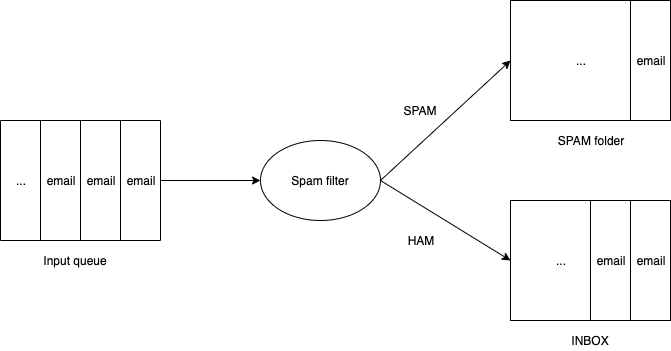
\includegraphics[width=0.8\linewidth]{SpamHam.png}
	\caption{Schematics of a spam filter system}
	\label{fig:spamham}
\end{figure}
Translating this example to a \textit{Machine Learning} classification requires extra functionalities.
Identifying all the different parameters that could point to one class or another and distribute a correct weight scheme upon them, opens up the possibility to translate a given entry into a point in space.
A \textit{Machine Learning} classification algorithm requires training data to find a certain border in space, where on one side the entries belong to one category, and on the other side not.
How this border is found depends heavily on the chosen algorithm, in this example the weight scheme is optimized so the border between categories could be linear. 
The decision making spam filter from figure~\ref{fig:spamham} contains the functionalities shown in figure~\ref{fig:spamhamML} .

\begin{figure}[H]
	\centering
	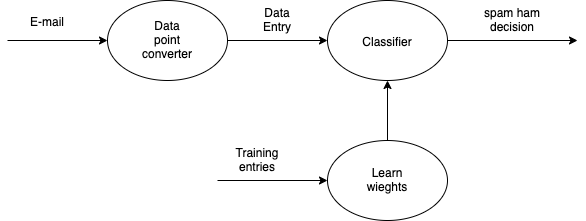
\includegraphics[width=0.8\linewidth]{SpamHamFilter.png}
	\caption{Schematics of a spam classification filter }
	\label{fig:spamhamML}
\end{figure}
The spam filer is an easy understandable example that provides a good entry into the field of \textit{Machine Learning}\cite{FlachPeter2012MLTA}
The following characteristics are presented in the above example and are considered the base of most to all algorithms.
\begin{itemize}
	\item The mathematical translation of a data entry to a point in space.
	\item The use of training data to construct a model.
	\item The will to optimize certain parameters. 
\end{itemize}

These can be further expanded with key concepts.\\
\textbf{Feature representation}: the translation from a data entry into a form where the algorithm can work with. 
Throughout the process it is not common to go back to the original data entry. 
What makes the use of feature representation so powerful is that the context and meta data of entries are abandoned.
In other words whether the data originates from chemical experiments or emails doesn't matter, after correct feature representation, the same algorithm can be used.\\
\textbf{Task} is the concept for an abstract representation of the problem that needs to be solved, this can be a classification, regression or other.\\
The output of a \textit{Machine Learning} algorithm is called a  \textbf{model}, this model is produced using training data and can be used to make a decision over future incoming data.
The model serves as a transformer between the input domain (translated to the feature space) $ x \in \mathscr{X}  $ and the output domain $ y \in \mathscr{Y}$.
With the input and output spaces having it's own specific dimensions.
\par 
Another important key concept is \textbf{overfitting}, this danger occurs when a model is made too close to the training data.
In other words only with input entries very close to the test data, the model will perform as assumed.
The model is over fitted to the training data and will not perform well in the general environment.
To prevent this from happening precautions can be taken.
One of those precautions is splitting the known data set into different smaller sets: a training set used to train the model, a validation set used by the model constructor itself to validate the model and a test set used to test the produced model.
This is shown in figure~\ref{fig:knownInstances}.
\begin{figure}[H]
	\centering
	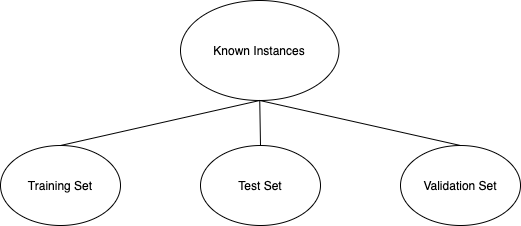
\includegraphics[width=0.8\linewidth]{KnownInstances.png}
	\caption{Splitting of the known instances set. }
	\label{fig:knownInstances}
\end{figure}

In general, \textit{Machine Learning} algorithms produce tools in the form of models to translate input data, meeting presupposed input dimensions and form, to a different presupposed output space, for filling the presupposed task.
Every translation has one correct answer, the produced model has the goal to find the correct answer for every input entry and is therefore an approximation to the perfect translation function.
$\hat{f}$ is the symbol for the model that approximates the true model $ f$ that in reality is maybe impossible to reach.
As mentioned earlier in this chapter, there are multiple categories in which \textit{Machine Learning} algorithms can be divided.
These categories are based on differences in functionality and output space, mostly related to the task.
In the following subsections two of those categories are discussed.

\subsection{Classification}
Classification algorithms classify input entries into one or more categories or classes.
The output space consists of a dimension corresponding to the number of classes.
When dealing with classification into to categories one can talk about binary classification.
Binary as in an output space consisting of 1 and 0, 1 for being part of a pre-assumed class, 0 for not being part or in other words being part of the complementary class.
The produced model for classification is called a \textbf{classifier} and provides a mapping $\hat{c}: \mathscr{X} \to \mathscr{L}$ with $\mathscr{L}$ being a finite small set containing the corresponding class labels and $\hat{c}$ being the approximation to the true classification function $ c$.
Examples, simulation, test or validation entries where the true classification is known are necessary to develop the $\hat{c}$ function.

\subsubsection{Binary Classification}
As stated above, binary classification is a classification into two different classes.
Further on, the different classes of the binary classification will be referred to as positive and negative.
After constructing a classifier and feeding it test data, a contingency table can be made, viewing the performance of the constructed classifier, as shown in table~\ref{tab:contingency}.
\begin{center}
	\begin{table}[H]
		\begin{tabular}{l|ll}
			& predicted + & predicted - \\ \hline
			Actual + &     (a)     &       (b)     \\
			Actual - &     (c)     &       (d)    
		\end{tabular}
		\caption{An example of a contingency table.}
		\label{tab:contingency}
	\end{table}
\end{center}
When discussing test results, the following key concepts are important to understand:
\begin{itemize}
	\item \textbf{True positive:} produced classifier predicted positive and real class value is positive, (a) in table~\ref{tab:contingency}. 
	\item \textbf{True negative:} produced classifier predicted negative and real class value is negative, (d) in table~\ref{tab:contingency}. 
	\item \textbf{False positive:} produced classifier predicted positive and real class value is negative, (c) in table~\ref{tab:contingency}. 
	\item \textbf{False negative:} produced classifier predicted negative and real class value is positive, (b) in table~\ref{tab:contingency}. 
\end{itemize} 
The accuracy of a model is the number of correct classified examples over the total number of examples and can, if the test set has a good data variety, be a good indicator for the probability that an incoming instance is classified in a correct way.\\
In the case that one class far outnumbers the other and the smaller preservative class actually determines a models performance, the accuracy is not a good measure to asses a models performance.
More characteristics can be calculated and used.
The \textbf{true positive rate} is the ratio of true positives over all actual positives. 
In similar fashion can the \textbf{true negative rate}, \textbf{false positive rate} and \textbf{false negative rate} be defined.
These characteristics determine the probability of correct (or falsely) classify entries to a specific class.
Giving a better insight when compared to accuracy if the problem stated above presents itself.
Another turn in performance evaluation is the characteristic \textbf{precision}.
Here the ratio of true positives is taken over the total predicted positives, giving insight in the resulting set of the positive class and giving an estimation of the probability that a classified entry of a certain class is in fact classified correctly.

\subsubsection{Multi-Class Classification}
Previously the binary classification is discussed. 
However most real life tasks consist of classifying entries into more than two classes.
Rather than starting from zero, it is more interesting and possible to expand the known characteristics and procedures, as discussed in binary classification into multi-class classification.
\par 
Imagine a classification into $k$ different classes. 
Different binary classifiers can be trained to find the fitness of an entry to every class.
This can be done with two different schemes, a \textbf{one-versus-rest} or a \textbf{one-versus-one} scheme.
In the one-versus-rest scheme $k$ or $k-1$ models are trained, depending on if the classes are in fixed order or not.
Each of those models separates one class from all the others.
In the one-versus-one scheme $k(k-1)/2$ or $k(k-1)$ amount of models are trained, depending on if the binary classifier treats the classes symmetrically or not. 
Each of them separating two classes.
The amount of classifiers created is referred to as $l$.
The $l$ different binary classifiers and $k$ different classes are combined in a so called $k$ by $l$ output code matrix. 
\par 
On a data entry, all the binary classifying models are run and make their own prediction.
This results in a set containing $l$ different values, one for each binary classifier.
The complete set is called a word. 
Translating this word into a decision is an extra step that was obviously not present previously for binary classifiers.
This process is called \textbf{decoding} and consists of finding the most suitable class for the code word.
Two very similar decoding schemes are distance-based and voting-based.
\par 
\textbf{Distance-based decoding:}\\
Every class row of the output code, called a class word, is compared to the code word.
A distance is calculated as presented in equation~\ref{eq:distancedecoding}:\\
\begin{equation}
	d(w,c_j)=\sum_{i=0}^{k} \left( 1 - w_i c_{ji}\right)/2
	\label{eq:distancedecoding}
\end{equation}
After iteration of all the class words, a most suitable class is chosen based on the minimal distance.
\par 
\textbf{Voting-based decoding:}\\
When working with a one-versus-one scheme, one can chose to use the voting-based decoding.
This is a very similar decoding scheme but instead of calculating distance "penalties", it is going to focus on votes in favor of a certain class.
After iteration of all the class words, a most suitable class is chosen based on the most votes.
\par 
\textbf{Loss-based decoding:}\\
This third decoding scheme is used when binary classifiers output scores instead of a clear decision.
The distance between every class word and the code word, here addressed as score word, is again calculated.
Instead of using equation~\ref{eq:distancedecoding}, the distance from every bit to the class bit is calculated by a loss function.
The correct calculation is shown in equation~\ref{eq:lossdecoding} with $s$ presenting the score word.
\begin{equation}
	d(s,c_j)=\sum_{i=0}^{k} L(s_i c_{ji})
	\label{eq:lossdecoding}
\end{equation}
After iteration of all the class words, a most suitable class is again chosen based on the lowest distance.

\subsection{Regression}
Where classifiers had discrete, finite output spaces, regression is a function estimator that can output any real value.
The goal of a regression algorithm is finding a function that best fits the given input data. 
When the modulated function resembles the training data too close, it is most likely that overfitting is going to occur.
The following rule can be applied: to avoid overfitting, the number of parameters estimated from the data must be considerably less than the number of data points.
In the sentence above, the word parameter is used, this referrers to the following.
The regressor is going to output a certain $n$-degree polynomial, the word parameter referrers to $n$.
The higher the polynomial degree, the better the test data is going to be resembled but the higher the chance that the modeled function is too specific.
\par 
For evaluating results with test sets, loss functions are applied. 
The input to this loss function is the difference between the actual know instance value and predicted value, these differences are called residuals.
Loss functions for regression models will be symmetric around zero, meaning that differences in any direction will result in the same loss function value.

\subsection{Bias-Variance Trade Off}
Difference in fits between data sets is called variance.
\textbf{Bias} is the amount in which the expected model differs from the true value, it is the individual error of a prediction.
Models with high bias values tent to underfit the training data. 
This is often a result from an over simplification.
An increase in complexity results in a decrease in error-rate.
\textbf{Variance} is defined as the amount a model would change if it would be estimated using a different set of training data.
High variance values point to an overfitting of the training data. 
In this case the created model resembles the training data too close, often this is the result of a model with a too high complexity rate, an increase in complexity results in an increase in error-rate.
\par 
The \textbf{Bias-Variance trade off} is defined as the point where the summation of bias and variance error rates are minimized.

\subsection{Cross Validation}
The term cross validation is used to describe a from of training.
This is an extension to the \textit{Machine Learning}, classification and regression functionalities.
According to the \textit{Machine Learning Encyclopedia} \cite{MachLearnEncy2017Spring}, Cross-validation is a process to train and validate the performance of a machine learning model.
Instead of developing one model and perform testing s on it, the known data set is divided into $k$-different chunks of data.
Each of these chunks or sub data sets, is referred to as a fold. 
$K$ different models are constructed, each of them using fold $S_i$ as testing set and a union of the other subsets as training data.
The performance results of the $k$ models are compared to increase the accuracy of the final output model.
\par 
Cross validation finds its origin in statistics and is applied in many different variations. 
Above the \textbf{k-fold cross-validation} is described and is commonly used in \textit{Machine Learning}.
Other variations are \textbf{leave-one-out}, \textbf{leave-p-out}, \textbf{Holdout method} and \textbf{Repeated random sub-sampling}.
Other variations and extensions on those also exist.
All of them have the same general goal: improving the accuracy of a generated \textit{Machine Learning} model by variation in testing and training data sets. 

\subsection{Support Vector Machines (SVMs)}
Support Vector Machines are introduced by Vapnik. 
The goal of an SVM algorithm is defining a hyperplane with the use of so called support vectors.
This hyperplane can be the separation between different classes or a function estimation and those support vectors find their origin in training data points. 
Previously described concepts are combined or extended in the so called SVMs.

\subsubsection{Kernel trick}\label{subsec:kerneltrick}
Support Vector Machines finds linear separators or linear functions to provide a solution.
In many cases it is not possible to separate data in a linear way or find a linear function estimation.
The provided solution maps the training data points into a different space.
In this so called \textit{High Dimensional Feature Space} or \textit{HDFS} it is possible to find linear solutions. \\
Mapping to the High Dimensional Feature Space is done by Kernel functions $K(x,z)$. 
Explicit mapping is not necessary, only the relations between data points in the \textit{HDFS} are calculated.
With $x$ and $z$ being two different data points.
The fact that a real transformation into a higher dimension is not necessary, is called the \textbf{Kernel Trick}, 
because of this trick, a linear solution can always be found AND finding a solution is not done in this higher dimension (finding solutions in higher dimension will always require more computational power).
This kernel function can be written as shown in equation~\ref{eq:kernel_base}.
\begin{equation}
	K(x,z) = \varphi(x)^T\varphi(z)
	\label{eq:kernel_base}
\end{equation}
with $\varphi(x)$ being the non linear mapping of data point x into the \textit{HDFS}.\\
Multiple functions can be used to do this non linear mapping, th most commonly used are listed below:
\begin{itemize}
	\item Linear kernel : $K(x,x_k) = x_k^Tx$
	\item Polynomial kernel of degree d : $K(x,x_k) = (\tau + x_k^T)^d$
	\item RBF kernel : $K(x,x_k) = e^{-\parallel x - x_k \parallel_2^2 / \sigma^2}$
	\item MLP kernel : $K(x,x_k) = \tanh(\kappa_1 x_k^T x + \kappa_2)$
\end{itemize}
Because of the kernel trick, use of the RBF kernel is possible. 
When using this kernel, the \textit{HDFS} can reach infinite dimension, finding a solution is only possible because this is not done in the \textit{HDFS}. 

\subsubsection{Classification}
Considering a binary classification problem, after plotting the data entries according to the features, the two classes can be separated by a hyperplane. 
This hyperplane is given by the following equation:
\begin{equation}
	\mid \omega^T x_k + b \mid = 0
\end{equation}
By definition the closest points to this hyper plane are meeting the following criteria:
\begin{equation}
	\mid \omega^T x_k + b \mid = 1
	\label{eq:supportvector}
\end{equation}
Because of this criteria, there consists a margin around the hyperplane, equal on both sides of the plane.
This margin is defined as:
\begin{equation}
	margin = \frac{2}{\parallel \omega \parallel_2}
\end{equation}
Support Vector Machines optimize their hyperplane definition by maximizing the margin.
In other words the larger the gap on both sides of the hyperplane the better the classification.
Maximizing the margin corresponds to minimizing the product of $\omega^T$ and $\omega$.
After introducing slack variable $\epsilon_k$ and kernel functions, the general form of the SVM classification has become:
\begin{equation}\footnote{Changing $\varphi(x)$ into $x$ changes the non linear classifier into a linear classifier.}
	y(x)=sign\left[\omega^T\varphi(x) + b \right]
	\label{eq:nonlinsvmclass}
\end{equation}
With $\omega$ and $b$ to be determined by an optimization solver.
This optimization problem can be defined in the primal weight space and after calculating the Lagrange multipliers, as a dual problem.
When solving the optimization problem as a dual problem, the following non linear SVM classifier has become:
\begin{equation}
	y(x) = sign\left[ \sum_{k=1}^{N} \alpha_k y_k K(x,x_k) + b \right]
	\label{eq:nonlinsvmclassifier}
\end{equation}
with: $\alpha$ being a Lagrange multiplier, $N$ being the total amount of training data entries and $K(x,x_k)$ being a kernel function.
In the linear case where the kernel trick is not used, equation~\ref{eq:nonlinsvmclassifier} has the following form:
\begin{equation}
y(x) = sign\left[ \sum_{k=1}^{N} \alpha_k y_k x^Tx + b \right]
\label{eq:linsvmclassifier}
\end{equation}
The Karush-Kuhn-Tucker (KKT) conditions are used to find the missing parameter $b$.
\par 
As described, two different optimization problems are defined. 
In the primal weight space, the goal is a minimization of the $\omega$, $b$ and $\epsilon$ values. 
However, $\omega$ will have the dimension equivalent to the hidden layer dimension, when using Kernel functions, this hidden layer dimension will increase\footnote{The hidden layer dimension can increase to infinity when using the RBF kernel.}, resulting in computational nightmare.
On the upside, the dimension of $\omega$ is independent to the training data size, meaning that solving the optimization problem in the primal weight space is preferred in the case of linear separable data with large training data sets.\footnote{Assuming that one knows if data is linear separable, knowing this upfront is very rare.}
In the dual problem, the goal is the maximization of the Lagrange multiplier $\alpha$.
This optimization problem is independent from the hidden layer dimension, when using Kernel functions this is the ideal way of finding the classifier parameters.
When using the dual space optimization, the classifier is shown in equation~\ref{eq:nonlinsvmclassifier}.
\par 
Earlier was mentioned that the term support vector, finds their origin in training data points. 
However not all training data points are support vectors.
Only those closest to the hyperplane are considered support vectors and have an $\alpha$ value different from zero.
This is very powerful because it limits the necessary iterations in the classifier considerably.
Training data points closest to the hyperplane are meeting the requirement shown in equation~\ref{eq:supportvector}.
With this knowledge the non linear classifier shown in equation~\ref{eq:nonlinsvmclassifier} can be modified into equation~\ref{eq:nonlinsvmmodclassifier}.
\begin{equation}
	y(x) = sign\left[ \sum_{k=1}^{\# SV} \alpha_k y_k K(x,x_k) + b \right]
	\label{eq:nonlinsvmmodclassifier}
\end{equation}
with $\# SV$ being the total number of support vectors.
Especially when dealing with larger training data sets this results in a favorable advantage.
\par 
Earlier in this document is described how performance of \textit{Machine Learning} can be analyzed. 
The introduced concepts are fully applicable on Support Vector Machine classification.
The same counts for the extension into multi-class classification. 
An SVM classifier is a binary classifier, which means that in the case of multi-class classification, the earlier described schemes can be used.
As well as the output code matrix and described concepts of decoding.

\subsubsection{Regression}
With regression or function estimation, the goal is not outputting a classifier, but a function estimation fitting the data as close and good as possible.
The described mechanisms in SVM classification can be slightly modified to fit the purpose of function estimation.
The resulting function can be written as shown in equation~\ref{eq:SVMregressionfunction}.
\begin{equation}\footnote{when Kernel functions are not used, $\varphi(x)$ can be changed into $x$.}
	f(x) = \omega^T \varphi(x) + b
	\label{eq:SVMregressionfunction}
\end{equation}
with:
\begin{itemize}
	\item $f(x)$: the outputted estimated function.
	\item $ \omega $: vector containing hidden layer weights, function parameter.
	\item $ x $ :input data entry.
	\item $ \varphi(.)$: non linear mapping function (Kernel functionality).
	\item $ b $ : function parameter.
\end{itemize}
With function estimation the risk of over fitting is real. 
When models are too complex or if the optimal solution is found for a certain training data set, the risk is real that the generated function is a too close match to the training data.
With this in mind, a loss function is defined, creating a region around the outputted function where data points are considered correctly fitted.
This function is called a Vapnik $\epsilon$-insensitive loss function and starts penalizing fittings outside of this so called correct band.
The course of this function is shown in figure~\ref{fig:einsensitive}.
\begin{figure}[H]
	\centering
	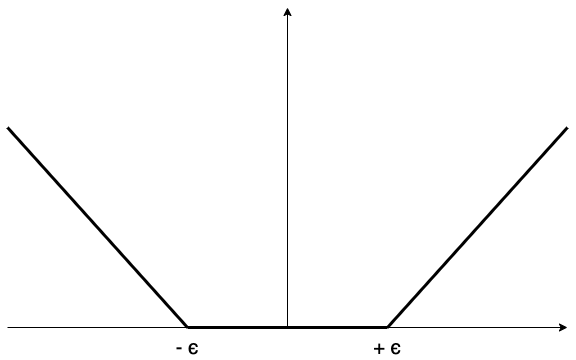
\includegraphics[width=0.6\linewidth]{e-insensitive.png}
	\caption{Course of the $\epsilon$-insensitive loss function}
	\label{fig:einsensitive}
\end{figure}
This function allows small misclassification to prevent overfitting. 
However training data points laying outside this acceptance band, referred to as outliers, will introduce an in feasibility to the problem.
Therefore are, in similar fashion to the SVM classifier, slack variables introduced, allowing miss-fittings.\\
An optimization problem is created in the primal weight space with the goal of minimizing the $\omega$ and slack variables.
After introducing the Lagrange multipliers, the primal weight space optimization problem can be modified to the dual problem, where a maximization is wanted of the Lagrange multipliers.
Resulting in the following dual representations of the model\footnote{Equation~\ref{eq:SVMregrepnonlin} presents the dual representation when using a kernel function and equation~\ref{eq:SVMregreplin} presents the representation without kernel function. }
\begin{equation}
	f(x) = \sum_{k=1}^{N}(\alpha_k-\alpha_k^*)K(x,x_k) + b
	\label{eq:SVMregrepnonlin}
\end{equation}
\begin{equation}
	f(x) = \sum_{k=1}^{N}(\alpha_k-\alpha_k^*)x^Tx + b
	\label{eq:SVMregreplin}
\end{equation}
with:
\begin{itemize}
	\item $\alpha_k$ and $\alpha_k^*$: Lagrange multipliers.
\end{itemize}
Again in similar fashion to SVM classification, the iterations can be reduced to only the support vectors.
\subsection{Conclusion}
Machine learning is a large scientific field.
The core concepts of classification, regression, modeling, error scores, and coding were discussed in this section.
Key concepts as the bias variance trade off and crossvalidation were introduced, important to have a good background knowledge of the basic machine learning concepts.
Besides the basic concepts, Support Vector Machines, designed by Vapnik, were discussed
SVMs make it possible to make a mathematical representation of an input data set by adding an extra layer: the high dimensional feature space.
Together with the basic concepts, this gives a general idea how SVMs can be used in practice to generate models for function estimation, classification and multi-classification.
\section{Optimization: Simulated Annealing and Coupled Simulated Annealing}
\subsection{Introduction}
In the field of optimization, many algorithms and technics finds their origin in other branches and fields.
Evolutionary algorithms as the biggest example, where the search space is iterated based on principles originating in biology and evolution theory \cite{Brabazon2015}.
The name search space is mentioned, optimization algorithms and heuristics iterate in a certain way through a space consisting of mathematical representations of possible solutions.
Linear problems can be solved by solving equations, however in many cases problems cannot be defined as combinations of linear equations. 
When the set of possible solutions becomes too large, iterating all possible solutions do not provide us with an elegant solution and requires an unnecessary computational power.
In this case heuristics and optimization algorithms offer valid alternatives. 
Here, the search space is iterated in a certain fashion with the goal of finding the optimal solution or a solution meeting minimal requirements without having the burden of the enormous computational power.
Inspiration for those methods originate, as mentioned, often in other scientific fields. 
Besides biology, physics also provides inspiration for the development of methods, the so called Physically Inspired Computing Algorithms \cite{Brabazon2015}.
The process of thermal annealing metal and glass is the base for the Simulated Annealing algorithm.\footnote{Annealing means a controlled cooling of materials in order to create higher quality products.}
\subsection{Simulated Annealing}
Assuming that all the solutions have some kind of mathematical representation, Simulated Annealing can be used to try to solve non convex optimization problems.
To understand this, one has to have basic knowledge of an annealing process.
In such a process a certain material (metal or glass) is cooled in a controlled environment, this means that the cooling rate as well as possible re-heating's are controlled by a system. 
Every state of the material corresponds to a certain energy level.
Throughout this process, several reheating moments are possible, resulting in a transfer of the material into a higher energy state.
Parameters that can be controlled in this process are the number of re-heatings, starting temperature, ending temperature, cooling rate, etc.
\par 
Firstly, it is important to understand that all heuristic search methods are in need of the following characteristics.
\begin{itemize}
	\item The search space, a mathematical representation of all possible solutions.
	\item An initial solution, provided by or a higher implementation or a random selection.
	\item A rating system for the solutions, often referred to as the cost of a function.
	\item General goal, the optimisation problem itself, often a minimisation or maximisation.
	\item Terminating condition, a stated criterium that when it is reached, stops the search for a solution.
	\item Generation of a new solution.
	\item Acceptance mechanism for a possible new solution.
\end{itemize} 
Translating the physical annealing process into an algorithmic idea requires the definition of some relations between the two.
\begin{itemize}
	\item Physical material states: Problem solutions
	\item Energy of a state: Solution cost
	\item Temperature: Control parameter
\end{itemize}
The search space, containing all possible solutions in vector representation, serves as an input to the algorithm.
Every possible solution is called a \textbf{state}, in relation with physical annealing.
The rating system can be build in into the algorithm or can be given in function form as a parameter.
This rating system is, in line with what is stated in the relations above, called the \textbf{energy} of a given state.
Meaning that the cost of a state $x$ is written as: $E(x)$. 
Another parameter is the start temperature $T_0$.
The \textbf{temperature} in the annealing process follows a predeterment cooling path.
Where in an annealing process the temperature path depends on the time, in simulated annealing this will be the number of iterated steps.
The variable temperature stands for an allowance when considering to accept a new possible solution. 
The more iteration passed, the lower the temperature will be, the smaller the allowance will become.
\par 
The \textbf{generation} of a new solution is partly dependent on a stochastic process. 
To form a next possible solution, a random vector with the same dimension of the vector presenting the current solution, is added to the current vector, where this random vector is picked out of a given distribution.\\
A possible new solution, $y$, is created.
The cost (Energy) of the new solution can be calculated: $E(y)$.
\par 
The \textbf{acceptance} of a new solution is done by a probability value.
When the cost of the possibly new solution $y$ is less than the cost of the current solution $x$, the acceptance probability is equal to 1.
However when the cost of $y$ is higher than the cost of $x$, $E(y)>E(x)$, the probability of acceptance can be calculated as shown in equation~\ref{eq:SAacceptanceProb}.
The implementation of the acceptance probability can show deviations depending on the implementation. However the principles remain the same: whether a move to a solution with a higher energy state is accepted is partly depended on the temperature.
The higher the temperature, the higher the resulting probability will be. 
In the simulated annealing heuristic, the temperature follows a cooling path, meaning that the chances that uphill moves will be accepted are higher in the beginning and will be lower after certain iterations.
Here exists a trade off, the slower the cooling down rate, the higher the chance the heuristic is going to come up with a good solution, but the longer the algorithm is going to take.
he temperature mostly follows a decreasing exponential path.
After every iteration, the new temperature value is calculated.\footnote{If unclear, an iteration is an attempt to accept a new solution regardless if the new solution is accepted.}Algorithm~\ref{alg:sa} presents a basic implementation of the simulated annealing algorithm.

\begin{equation}
	P(x \rightarrow y) = e^{(-\Delta f/T_y)}
	\label{eq:SAacceptanceProb}
\end{equation}



\begin{algorithm}[H]
	\fbox{\begin{minipage}{\linewidth}
	\SetKwInOut{Input}{input}\SetKwInOut{Output}{output}
	\Input{Search Space $sesp$,\\ Starting Temperature $T_0$,\\ Cost Function $E(.)$,\\ Temperature Schedule $U()$}
	\Output{Solution $s$ }
		
	// initialization \\
	$x$ = sesp(random)\;
	$T$ = $T_0$\;
	$k$ = $0$\;
		
	\Repeat{Until Stop conditions}{
		// Generate new solution \\
		$\varepsilon$ =random()
		$y$ = generate($\varepsilon$,$T$)\;
		// Acceptance \\
		\eIf{$E(y)<E(x)$}
		{$x$ = $y$\;}
		{$p$ = probCalc($E(x)$,$E(y)$,$T$)\;
		Accept with probabilty $p$}
	// Decrease temperature \\
	$k++$\;
	$T$ = $U(T,k)$
	}
	\end{minipage}}
		
	\caption{Basic implementation of the Simulated Annealing algorithm.}
	\label{alg:sa}
\end{algorithm}
In two places, generation of a new solution and acceptance, the algorithm is dependent on a stochastic variable.
Therefore a reheating of the algorithm can result in a different and or better final solution.

\subsection{Coupled Simulated Annealing}
With large amount of iterations and multiple reheatings, the simulated annealing process can have a time complexity that rises above what is still interesting.
An available extension is called coupled simulated annealing \cite{csa2007}.
Coupling local optimization possibilities will increase the chances of escaping local optima and the coupling functions lent to an efficient implementation in parallel architectures. \cite{CoLoMi2002} \cite{csa2007}
These two are very important and appealing upsides, making this a very interesting extension to the simulated annealing heuristic.
\par 
The following notations will be used:
\begin{itemize}
	\item $m$: number of coupled elements.
	\item $\Omega$: search space containing all solutions.
	\item $\Theta$: subset of the search space.
	\item $\gamma$: coupling term, scalar value calculated by a function depending on the energy of the elements in $\Theta$.
	\item $A_\Theta (\gamma,x_i \rightarrow y_i)$: scalar presenting the acceptance probability of the new presented solutions.
\end{itemize}
In CSA $m$ different processes start their search for a better solution, they are coupled to each other in the acceptance phase of the algorithm.
Where in simulated annealing the probability of acceptance is a scalar value based on a single possible transition, in CSA this is based on $m$ possible transitions to new solutions AND a coupling term $\gamma$.
\par 
To change the SA algorithm to its CSA version, a change in every step of the algorithm is required.
In the \textbf{initialization} phase, $m$ different randomly selected solutions need to be created.
Together they make $\Theta$ a subset of $\Omega$.
In the \textbf{generation} phase, $m$ new solutions are selected, each in the neighbourhood of its current solution.
In the \textbf{acceptance} phase, the probability of acceptance for every new solution is calculated. 
The acceptance probabilty equation does not only depend on the energy levels of the solutions but also on the coupling factor.
Before entering the \textbf{temperature decrease} phase, the generation and acceptance phase are iterated $N$ times, this number of iterations are called inner iterations.
In the temperature decrease phase, the temperature is decreased according to a certain scheme, similar to SA.
In the \textbf{stop criterium} phase, the criterium is calculated, if its met, the excecution stops here, otherwise the algorithm returns to the generation phase.
\par 
Both the probability function and couple parameter are not fixed functions, resulting in a certain form of freedom when implementing CSA.
Implementations based on these principles are \textbf{Multi-State Simmulated Annealing (CSA-MuSA)}, \textbf{Blind Acceptance (CSA-BA)}, \textbf{CSA Modified (CSA-M)} and after more modifications \textbf{CSA-MwVC}.
\subsubsection{Multi-State Simmulated Annealing (CSA-MuSA)}
Direct generalisation of the SA algorithm.
The acceptance function has the form of the CA acceptance function, but generalised to include more states, hence the name Multi State CSA.
Equation~\ref{eq:CSAMSacceptprob} shows the probability acceptance function and equation~\ref{eq:CSAMScouple} shows the coupling term function.
\begin{equation}
	A_\Theta(\gamma,x_i \rightarrow y_i)=\frac{\exp(\frac{-E(y_i)}{T_k})}{\exp(\frac{-E(y_i)}{T_k})+\gamma}
	\label{eq:CSAMSacceptprob}
\end{equation}
\begin{equation}
	\gamma = \sum_{x_j \in \Theta}^{}\exp(\frac{-E(x_j)}{T_k})
	\label{eq:CSAMScouple}
\end{equation}
\subsubsection{Blind Acceptance (CSA-BA)}
For blind acceptance CSA, the probability function is given in equation~\ref{eq:CSABAacceptprob} and for the coupling term, the same equation as in Multi State is used, equation~\ref{eq:CSAMScouple}.
What stands out is the fact that the acceptance is only depended on the energy of the current states and not of the new selected once.
Resulting out of this fact, is that low energy states accept fewer uphill moves than higher energy states.
Because of the fact that only current energy states are considerer, this version is called blind acceptance.
\begin{equation}
	A_\Theta(\gamma,x_i \rightarrow y_i)=1 - \frac{\exp(\frac{-E(x_i)}{T_k})}{\gamma}
	\label{eq:CSABAacceptprob}
\end{equation}
\subsubsection{CSA Modified (CSA-M)}
CSA Modified tries to combine the upsides of both CSA-MuSa and CSA-BA. 
The probability function used in CSA-M is shown in equation~\ref{eq:CSAMacceptprob}, it is a modified and normalised version of the function used in CSA-BA, equation~\ref{eq:CSABAacceptprobnn}.
Here the focus is also on the probability of leaving the current solution, however the positive energy is considered what can lead to stability issues.
Therefore, the probability and couple functions are normalised in relation to the highest amount of energy present in $\Theta$.
The couple function is shown in equation~\ref{eq:CSAMcouplenn}, together with it's normalised version in equation~\ref{eq:CSAMcouple}
\begin{equation}
	A_\Theta(\gamma,x_i \rightarrow y_i)= \frac{\exp(\frac{E(x_i)}{T_k})}{\gamma}
	\label{eq:CSABAacceptprobnn}
\end{equation}
\begin{equation}
	\gamma = \sum_{x_j \in \Theta}^{}\exp(\frac{E(x_j)}{T_k})
	\label{eq:CSAMcouplenn}
\end{equation}
\begin{equation}
	A_\Theta^*(\gamma^*,x_i \rightarrow y_i)=\frac{\exp \left( \frac{E(x_i)-\max\limits_{x_i \in \Theta}(E(x_i) ) }{T_k} \right)   }{\gamma^*}
	\label{eq:CSAMacceptprob}
\end{equation}
\begin{equation}
	\gamma^* = \sum_{x_j \in \Theta}^{} \exp \left( \frac{E(x_i)-\max\limits_{x_i \in \Theta}(E(x_i) ) }{T_k} \right)   
	\label{eq:CSAMcouple}
\end{equation}
This formulation results, in the case of low temperatures, into a high probability for leaving a current solution when the energy value is high, where probabilities will be close to zero in the case of low energy values.
\subsubsection{CSA Modified with Variance Control (CSA-MwVc)}
Out of observations and experiments \cite{csa2007}, the conclusion can be made that the optimisation performs best when the variance is close to the upper bound.
The variance can be controlled by adjusting the temperature. 
Because the temperature value is present in both numerator and denominator, it is the perfect variable to control in order to have control over the probability variance.
The probability variance $\sigma^2$ is calculated as shown in equation~\ref{eq:CSAMwVCvariance}, where it's bound values are shown in equation~\ref{eq:CSAMwVCvariancebound}.
In order to control the variance, the algorithm used in the previous CSA implementations is taken and slightly adjusted.
The adjustment of temperature takes places after all the $N$ inner iterations are completed and before the generation temperature is adjusted.
For the adjustment, the acceptance temperature is updated as shown in equation~\ref{eq:CSAMwVCvariancetempupdate}.\footnote{Where in the previous CSA implementations only one type of temperature could do the trick, here it is absolutely necessary to have two types of temperature: generation temperature and acceptance temperature.\cite{csa2007}}
Where $\sigma_D^2$ is the desired variance value and $\alpha$ a process parameter usually between $0$ and $0.1$.
\begin{equation}
	\sigma^2 = \frac{1}{m}\sum_{\forall x_i \in \Theta}^{} A_\Theta^2 - \frac{1}{m^2}
	\label{eq:CSAMwVCvariance}
\end{equation}
\begin{equation}
	0 \leq \sigma^2 \leq \frac{m - 1}{m^2}
	\label{eq:CSAMwVCvariancebound}
\end{equation}
\begin{equation}
	\begin{split}
		if  \sigma^2 < \sigma_D^2: T_k^{ac}=T_{k-1}^{ac}(1 - \alpha) \\
		if  \sigma^2 > \sigma_D^2: T_k^{ac}=T_{k-1}^{ac}(1 + \alpha)
	\end{split}
	\label{eq:CSAMwVCvariancetempupdate}
\end{equation}
 
\subsection{Conclusion}
Simulated annealing provides a good heuristic in the world of non-convex optimisation problems.
However it is not parallel executing friendly and in case of multiple re-heatings the computing time increases heavily. 
Coupled Simulated Annealing provides a solution where multiple Simulated Annealing process are coupled to each other. 
This introduces parallel computing possibilities.
Because the processes are coupled in acceptance, the overall performance will increase.
A side note while looking at the future\footnote{The future is parallel computing.}, the coupling of acceptance and the need for all the energy values, limits the possible acceleration when the CSA process is implemented in a parallel computing environment.

\section{Least-Square Support Vector Machines (LS-SVM)}
\subsection{Introduction}
The Least Square Support Vector Machines algorithm is designed by Suykens et al. and uses the elements explained in the previous sections. \cite{Suykens2002}
In LS-SVM the problem formulation is simplified to a minimization searchproblem as shown in equation~\ref{eq:lssvmobjective}.
With:
\begin{equation}
	\begin{split}
		minimize_{\omega,b,e} = \frac{1}{2} \omega^T \omega + \frac{\gamma}{2} \sum_{k=1}^{N}e^2_k \\
		y_k \left[\omega_T \varphi(x_k)+b\right]=1-e_k, \qquad k = 1,\dots,N
	\end{split}
	\label{eq:lssvmobjective}
\end{equation}
\subsection{Differences and Solving}
The fundamental differences with a normal SVM approach can be found in the constraints and the loss functions.
Where SVM uses inequalities as constraints, the lssvm approach uses equalities. 
The use of equalities makes it easier to compute possible solutions.
In the loss function, the squared loss is calculated. 
This enhances the significances of big losses in the minimization factor.
Completely in line with the SVM principles, a solution can by formulating the problem into the dual space.\cite{Suykens2002}
As described by Suykens et al. the Lagranian is formulated in equation~\ref{eq:lssvmlagranian}.
\begin{equation}
	\mathscr{L}(\omega,b,e;\alpha)=\frac{1}{2}+ \frac{\gamma}{2} \sum_{k=1}^{N}e^2_k - \sum_{k=1}^{N}\alpha_k\left\{ y_k\left[\omega^T\varphi(x_k) + b\right] - 1 + e_k \right\}
	\label{eq:lssvmlagranian}
\end{equation}
Following from the Lagrangian equation are the following constraints.
\begin{equation}
	\begin{cases}
		\frac{\delta \mathscr{L}}{\delta \omega} = 0 \to \omega = \sum_{k=1}^{N}\alpha_k y_k\varphi(x_k) \\
		\frac{\delta \mathscr{L}}{\delta b} = 0 \to \sum_{k=1}^{N}\alpha_k y_k = 0 \\
		\frac{\delta \mathscr{L}}{\delta e_k} = 0 \to \alpha_k=\gamma e_k \qquad k = 1,\dots,N\\
		\frac{\delta \mathscr{L}}{\delta \alpha_i} = 0 \to  y_k\left[\omega_T\varphi(x_k) + b \right] - 1 + e_k = 0 \qquad i = k,\dots,N
	\end{cases}
	\label{eq:lssvmlangranianconditions}
\end{equation}
In the previous three equations, a certain amount of variables are used, before continuing it might be useful to ensure the right perspective on those variables.
\begin{itemize}
	\item $\omega$: In relation with previous sections, when talking about $\omega$, we talk about the, to be found, weight vector.
	\item $e_k$: error for element $k$.
	\item $b$: calculated offset.
	\item $\varphi(x_k)$: representation of data entry point $X_i$ in the kernel specific domain, see kernel trick.
	\item $\gamma$: relative importance of error factor, possible outcomes are either minimizing the error or penalizing larger weights. $\gamma > 0$
	\item $\alpha$: Lagrangian multipliers, limited by condition three of equation~\ref{eq:lssvmlangranianconditions}.
\end{itemize}
From the conditions in equation~\ref{eq:lssvmlangranianconditions}, $\omega$ and $e$ can be eliminating. 
The following linear system can be solved:
\begin{equation}
	\left[
	\begin{array}{c|c}
	0 & 1_n^T \\ 
	\hline
	1_n & \Omega +\frac{1}{n}I_n
	\end{array}
	\right]
	\left[
	\begin{array}{c}
	b\\
	\hline
	\alpha
	\end{array}
	\right]
	=
	\left[
	\begin{array}{c}
	0\\
	\hline
	Y
	\end{array}
	\right]
\end{equation}
$\Omega$ is the representation of the kernel matrix as shown in section~\ref{subsec:kerneltrick}.
\begin{equation}
	\begin{split}
		\Omega_{kl} = y_k y_l \varphi(x_k)^T \varphi(x_l) \\
		= y_k y_l K(x_k, x_l)
	\end{split}
\end{equation}
With $k$ and $l$ ranging from $1$ to $N$.
The classifier is formulated in the following way:
\begin{equation}
	y(x) = sign \left[\sum_{i=1}^{n} \alpha_k y_k K(x,x_k) + b\right]
	\label{eq:lssvmclassifier}
\end{equation}
With equation~\ref{eq:lssvmmodel} presenting the model.
\begin{equation}
	model = \left[\sum_{i=1}^{n} \alpha_k y_k K(x,x_k) + b\right]
	\label{eq:lssvmmodel}
\end{equation}
Solving  a linear system is easier and requires less computational power than solving a quadratic programming problem. 
However, this simplified formulation results in a loss of sparseness. 
This is clearly visible in the Lagrangian optimal condition $\alpha_k =\gamma e_k$.
No $\alpha_k$ values will be zero, resulting in the fact that the LS-SVM approach uses all data points as Support Vectors.
\subsection{Parameter optimization}
Solving the linear system results in a solution for $\alpha$ and $b$.
Other parameters need to be found in a different manner.
The first parameter is $\gamma$, as shown in equation~\ref{eq:lssvmobjective}.
When making use of the kernel trick, a certain kernel type has to be chosen.
If the choice for RBF-kernel is made, the parameter $\sigma$ makes it introduction.
The parameters $\gamma$ and $\sigma$ can be calculated in different ways.
One way is working with a training, validation en test set to reduce the parameter possibilities to a smaller grid.
Statistically better, but computational heavier is the parameter and hyper parameter calculation by Bayesian inference. 
This is computational heavier because cross validation is used to find the parameter values with the best performance. 
\subsection{Conclusion}
The LS-SVM algorithm is based on the SVM logic, but altered to provide a more suitable algorithm.
Sacrifices are made in sparseness and new elements in the form of parameter tuning are introduced.
\section{Fixed Size Least Square Support Vector Machines (FS LS-SVM)}
\subsection{Introduction}
Fixed Size Least Square Support Vector Machines (FS LS-SVM) algorithm is also introduced by Suykens et al. \cite{Suykens2002} and is a variation from the LS-SVM algorithm.
The term Fixed Size stands for a fixed size of support vectors. 
Meaning that the sacrifice made in LS-SVM in the field of sparseness can be made undone here.
Typically FS LS-SVM is used in problems with larger data sets because standard LS-SVM does not perform well.
The problems with LS-SVM and large data sets are the following:
\begin{itemize}
	\item Because of the sparseness compromise, the algorithm considers every point a support vector. 
	Therefore the kernel matrix can grow with a higher than linear factor, making it an unrealistic method for large data sets. In other words, the memory complexity of the kernel matrix is too high. \footnote{An exact  number cannot be given at this point because it is related to the chosen kernel type.}
	\item In the dual space, the solution size is proportional to the size of the data set. 
\end{itemize}
In FS LS-SVM these problems are dealt with by introducing new and other elements.
\subsection{Mathematical Background and Algorithm}
As shown in figure~\ref{fig:fslssvmDetailedOverview} the FS LS-SVM algorithm consists of different stages.
The first stage is newly introduced because of the fixed size support vectors.
From this moment on, the number correlating to \textit{fixed size}, will be called $m$ and the total amount of data points will be $N$.
\begin{figure}
	\centering
	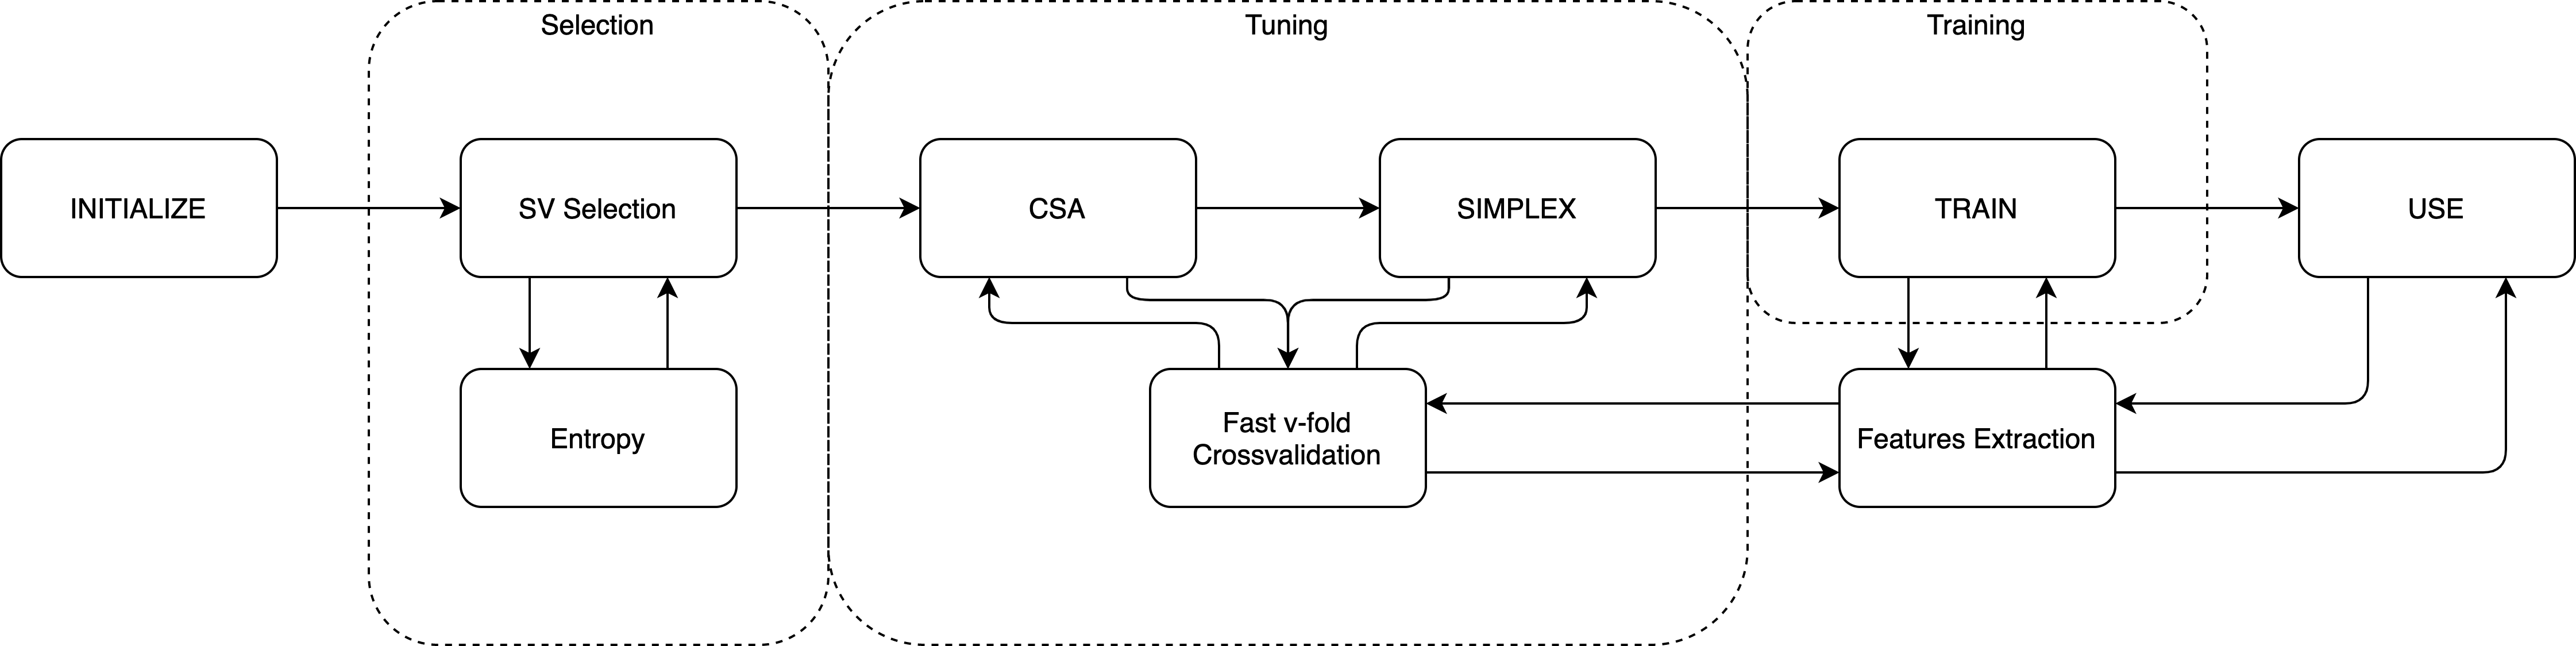
\includegraphics[width=\linewidth]{fslssvmPhases}
	\caption{Overview of the different phases and blocks of the FS LS-SVM algorithm.}
	\label{fig:fslssvmDetailedOverview}
\end{figure}
\subsubsection{Support Vector Selection}
When choosing a subsample of all the available data points as support vectors, the kernel matrix can be build only upon this sub sample.
In other words the kernel matrix build from the subsample has to be a good representation of the normally build matrix upon the complete set. 
The same objective function is used, as shown in equation~\ref{eq:lssvmobjective}, but the factor $\varphi()$ will be changed to $\hat{\varphi}()$. 
Meaning that $\hat{\varphi}()$ is the feature map representation of a subset of the total available data points.
This feature map can be build using the Nystr\"{o}m method.
The Nystr\"{o}m method will build a kernel matrix representation ($\Omega$) of size $m$, that is a good approximation of the kernel matrix of size $N$, usually $m<<<N$.
The memory complexity of the kernel matrix is now independent from the number of data points.
This has the result that it is much more suitable to calculate models for large data sets.
\par
The search for a good set of support vectors consists of several steps.
Before explaining these steps it is clear we need some kind of classification for every subset that we consider.
The classification parameter proven worthy is entropy, especially R\'{e}nyi entropy.
An entropy value represents the diversity or randomness of a system (or in this case dataset).
This is an interesting classifier because we want the subset of data points to be as diverse as possible.
Why? Because a diverse subset gives a better representation of the complete dataset and are therefore better candidates for support vectors.
The calculation of the R\"{e}nyi entropy is shown in equation~\ref{eq:renyientropy}.
\begin{equation}
	H_R^{(q)}(x)=\frac{1}{1-q}\log\int f(x)^q dx
	\label{eq:renyientropy}
\end{equation}
Where $f()$ is a density function and the factor $q$ stands for the power of the entropy.
Suykens et al. speak about quadratic R\'{e}nyi entropy \cite{Suykens2002}, meaning $q=2$.
This transforms equation~\ref{eq:renyientropy} into equation~\ref{eq:quadraticrenyientropy}.
\begin{equation}
H_R^2(x)=-\log\int f(x)^2 dx
\label{eq:quadraticrenyientropy}
\end{equation}
In order to calculate an entropy value for a certain subset, the density has to be known, presented by $f(x)$.
The density factor can be calculated by directly using the kernel function. 
The classification mechanism is explained, than we can go on to explain the steps that need to be taken in order to get a good support vector selection.\\
Support Vector Selection Mechanism:\cite{Suykens2002}\\
\begin{enumerate}
	\item Select random subset of size $m$ out of $N$ data points, calculate their entropy value.
	\item Select a random data point in this subset, lets call it $x_k$ and select a random data point outside the current subset, lets call it $x_l$. Swap $x_k$ and $x_l$
	\item Recalculate entropy value, if the entropy value increased, accept the swap otherwise reject it.
	\item Repeat step 2 to 4 until increase in entropy becomes too small or until the max number of iterations is completed.
\end{enumerate}
Note that the number of iteration is highly dependent on the threshold given for too small increase, and the max iteration number given.
A second consideration is the value of $m$.
As shown by De Brabander et. al \cite{Optimized2010:article}, methods with a high computational complexity are available to provide a good estimation for $m$, but those are not attractive for large data sets.
The choice for both $m$ as the max iteration value is made by following some ground rules in this thesis. 
More on that later.
\subsubsection{Parameter Tuning}
As shown in figure~\ref{fig:fslssvmoverview} the next phase in the the FS LS-SVM algorithm is the parameter tuning.
Even with a fixed number of support vectors, the tuning phase is a computational very heavy phase.
The parameters that have to get a value are: regularization parameter $\gamma$ and the kernel bandwidth $\sigma$ in case the RBF kernel is chosen.
The algorithm uses a Coupled Simulated Annealing search heuristic to find a grid of good parameter value couples, followed the simplex  algorithm to fine tune and choose the optimal parameters.
The elements CSA an simplex both need a cost function to validate the possible parameter values.
In FS LS-SVM the cost function used is a crossvalidation function. 
Crossvalidation functions are computational heavy functions, a model has to be trained for every \textit{fold}.
This is necessary because every fold uses a different set of training data points and validation data points.
In the optimized FS LS-SVM version, a special crossvalidation function is used in order to reduce the amount and complexity of matrix computations needed: \textit{fast v-fold crossvalidation}.\cite{Optimized2010:article}
Figure~\ref{fig:fslssvmtuningphase} shows the different steps in a tuning phase.
\begin{figure}
	\centering
	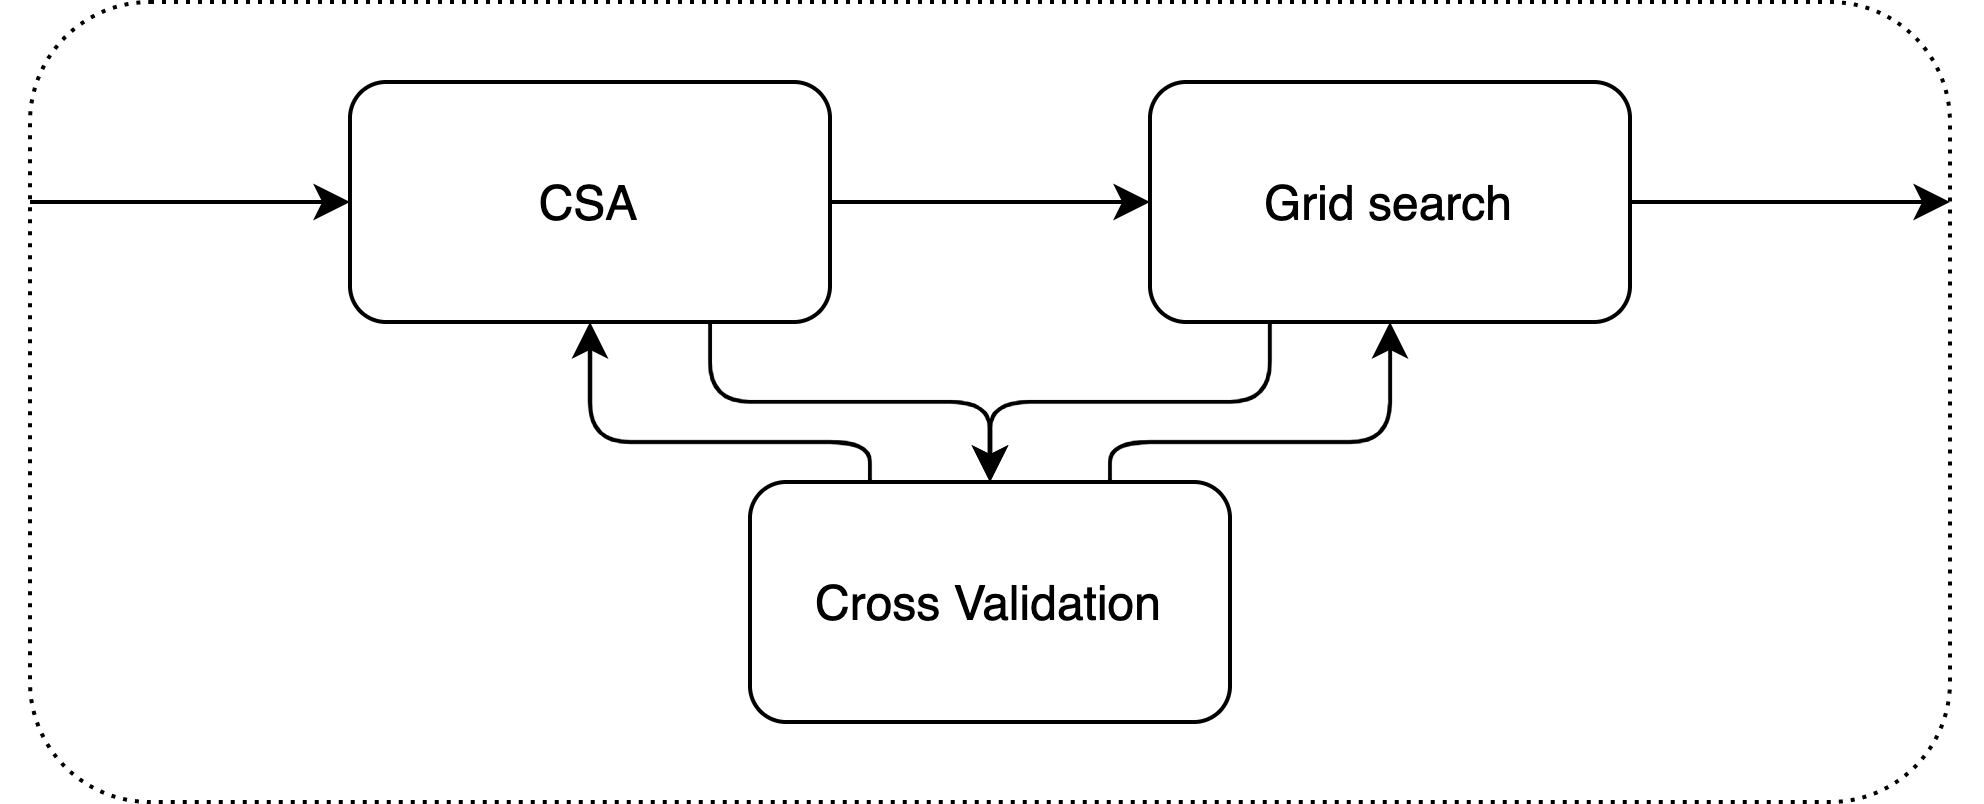
\includegraphics[width=0.8\linewidth]{TuningPhase.png}
	\caption{The different steps in a tuning phase.}
	\label{fig:fslssvmtuningphase}
\end{figure}
\subsubsection{Fast $v$-fold Crossvalidation}\label{subsec:fastvfoldcv}
This particular version of the crossvalidation principle is designed with reduction of needed computational complexity in mind.
Figure~\ref{fig:fastvfoldcrossvalidationoverview} shows a detailed overview of all the different steps.
Before diving in, we can define three different regions: Nystr\"om method, pre fold and v-fold.
The Nystr\"om method is part of the pre fold region.
It is important to understand that the pre fold region is not taken into the loop.
This means that only the v-fold region is going to be executed in a loop, more specific $v$ times.
\par
Before diving into the different elements, a little bit of a context is required.
The goal of the crossvalidation algorithm is determing the cost of a model over $v$ folds.
In order to compute this cost, the linear model has to be created. 
The parameters $\hat{\omega}$ and $\hat{b}$ need to be found. 
Finding these parameters can be done by solving the linear system shown in equation~\ref{eq:linearsystemfastfold}
\begin{equation}
	\binom{\hat{w}}{\hat{b}} = \left( \hat{\Phi}_e^T\hat{\Phi}_e + \frac{I_{m+1}}{\gamma} \right)^{-1} \hat{\Phi}_e^TY
	\label{eq:linearsystemfastfold}
\end{equation}
Equation~\ref{eq:linearsystemfastfold} can be reduced to equation~\ref{eq:linearsystemfastfoldreduced}, with the definitions of matrix $A$ (equation~\ref{eq:A})and vector $c$ (equation~\ref{eq:c}).
\begin{equation}
	\binom{\hat{w}}{\hat{b}} = \left( A \right)^{-1} c
	\label{eq:linearsystemfastfoldreduced}
\end{equation}
\begin{equation}
	A = \hat{\Phi}_e^T\hat{\Phi}_e + \frac{I_{m+1}}{\gamma}
	\label{eq:A}
\end{equation}
\begin{equation}
	c = \hat{\Phi}_e^TY
	\label{eq:c}
\end{equation}
Important note: $\hat{\Phi}_e$ is the extended feature matrix, where the normal feature matrix has a dimension of $n$x$m$, the extended feature matrix has a dimension of $n$x$m+1$, a vector of 1s is added as dimension $m+1$.
The introduction of $A$ and $c$ are important and needed because they make something else possible.
Imagine for every fold the feature matrix can be split into $\hat{\Phi}_{e,tr}$ and $\hat{\Phi}_{e,v}$, corresponding to the training block and the validation block.
Keep in mind that the training block is substantially larger compared to the validation block.
Equations~\ref{eq:Av}  can be made, and further reduced to equations~\ref{eq:Avreduced} and~\ref{eq:cvreduced}.
\begin{equation}
\hat{\Phi}_{e,tr}^T\hat{\Phi}_{e,tr} + \frac{I_{m+1}}{\gamma} = \left(  \hat{\Phi}_e^T\hat{\Phi}_e + \frac{I_{m+1}}{\gamma} \right) - \left( \frac{\hat{\Phi}_{val}^T}{1_{val}^T}\right) \left( \hat{\Phi}_{val} \middle| 1_{val} \right)
\label{eq:Av}
\end{equation}
\begin{equation}
A_v = A - \left( \frac{\hat{\Phi}_{val}^T}{1_{val}^T}\right) \left( \hat{\Phi}_{val} \middle| 1_{val} \right)
\label{eq:Avreduced}
\end{equation}
\begin{equation}
c_v = c - \left( \frac{\hat{\Phi}_{val}^T}{1_{val}^T}\right) Y_{val}
\label{eq:cvreduced}
\end{equation}
Because $A$ and $c$ only have to be calculated once for $v$ folds and $A_v$ and $c_v$ only depend on computations with the small validation set, the amount of computations is drastically reduced.
Hence the name \textit{fast v-fold crossvalidation}.
\paragraph{Feature Extraction using the Nystr\"om method}
The feature matrix can be calculated by using equation~\ref{eq:nystrom1}.
In order to compute this, the kernel matrix based on the support vector selection $\Omega$ is needed, as well as the kernel matrix representing the bridge between the complete data set and the support vectors $\Omega_N$ and the eigendecomposition of matrix $\Omega_N$.
\begin{equation}
\hat{\Phi_e}= repmat(\frac{1}{\sqrt{eigvals(\Omega)}},n).*\Omega_N eigvecs(\Omega)
\label{eq:nystrom1}
\end{equation}
The computation of both $\Omega$ and $\Omega_N$ depends on the kernel function used.
Equation of the most commonly used kernels can be found in section~\ref{subsec:kerneltrick}.
\paragraph{Prefold} 
After extracting the feature matrix, this one has to be extended and the values for $A$ and $c$ can be calculated.
the $v$ folds can now start and take $A$, $c$ and $\hat{\Phi}_e$ as input values.
\paragraph{v folds}
For every fold $A_v$ and $c_v$ are calculated, followed by the values for $\hat{\omega}$ and $b$.
These values are calculated by solving the linear system in equation~\ref{eq:linsystem}.
\begin{equation}
	\binom{\hat{\omega}}{b} = A_v^-1c_v
	\label{eq:linsystem}
\end{equation}
\begin{figure}
	\centering
	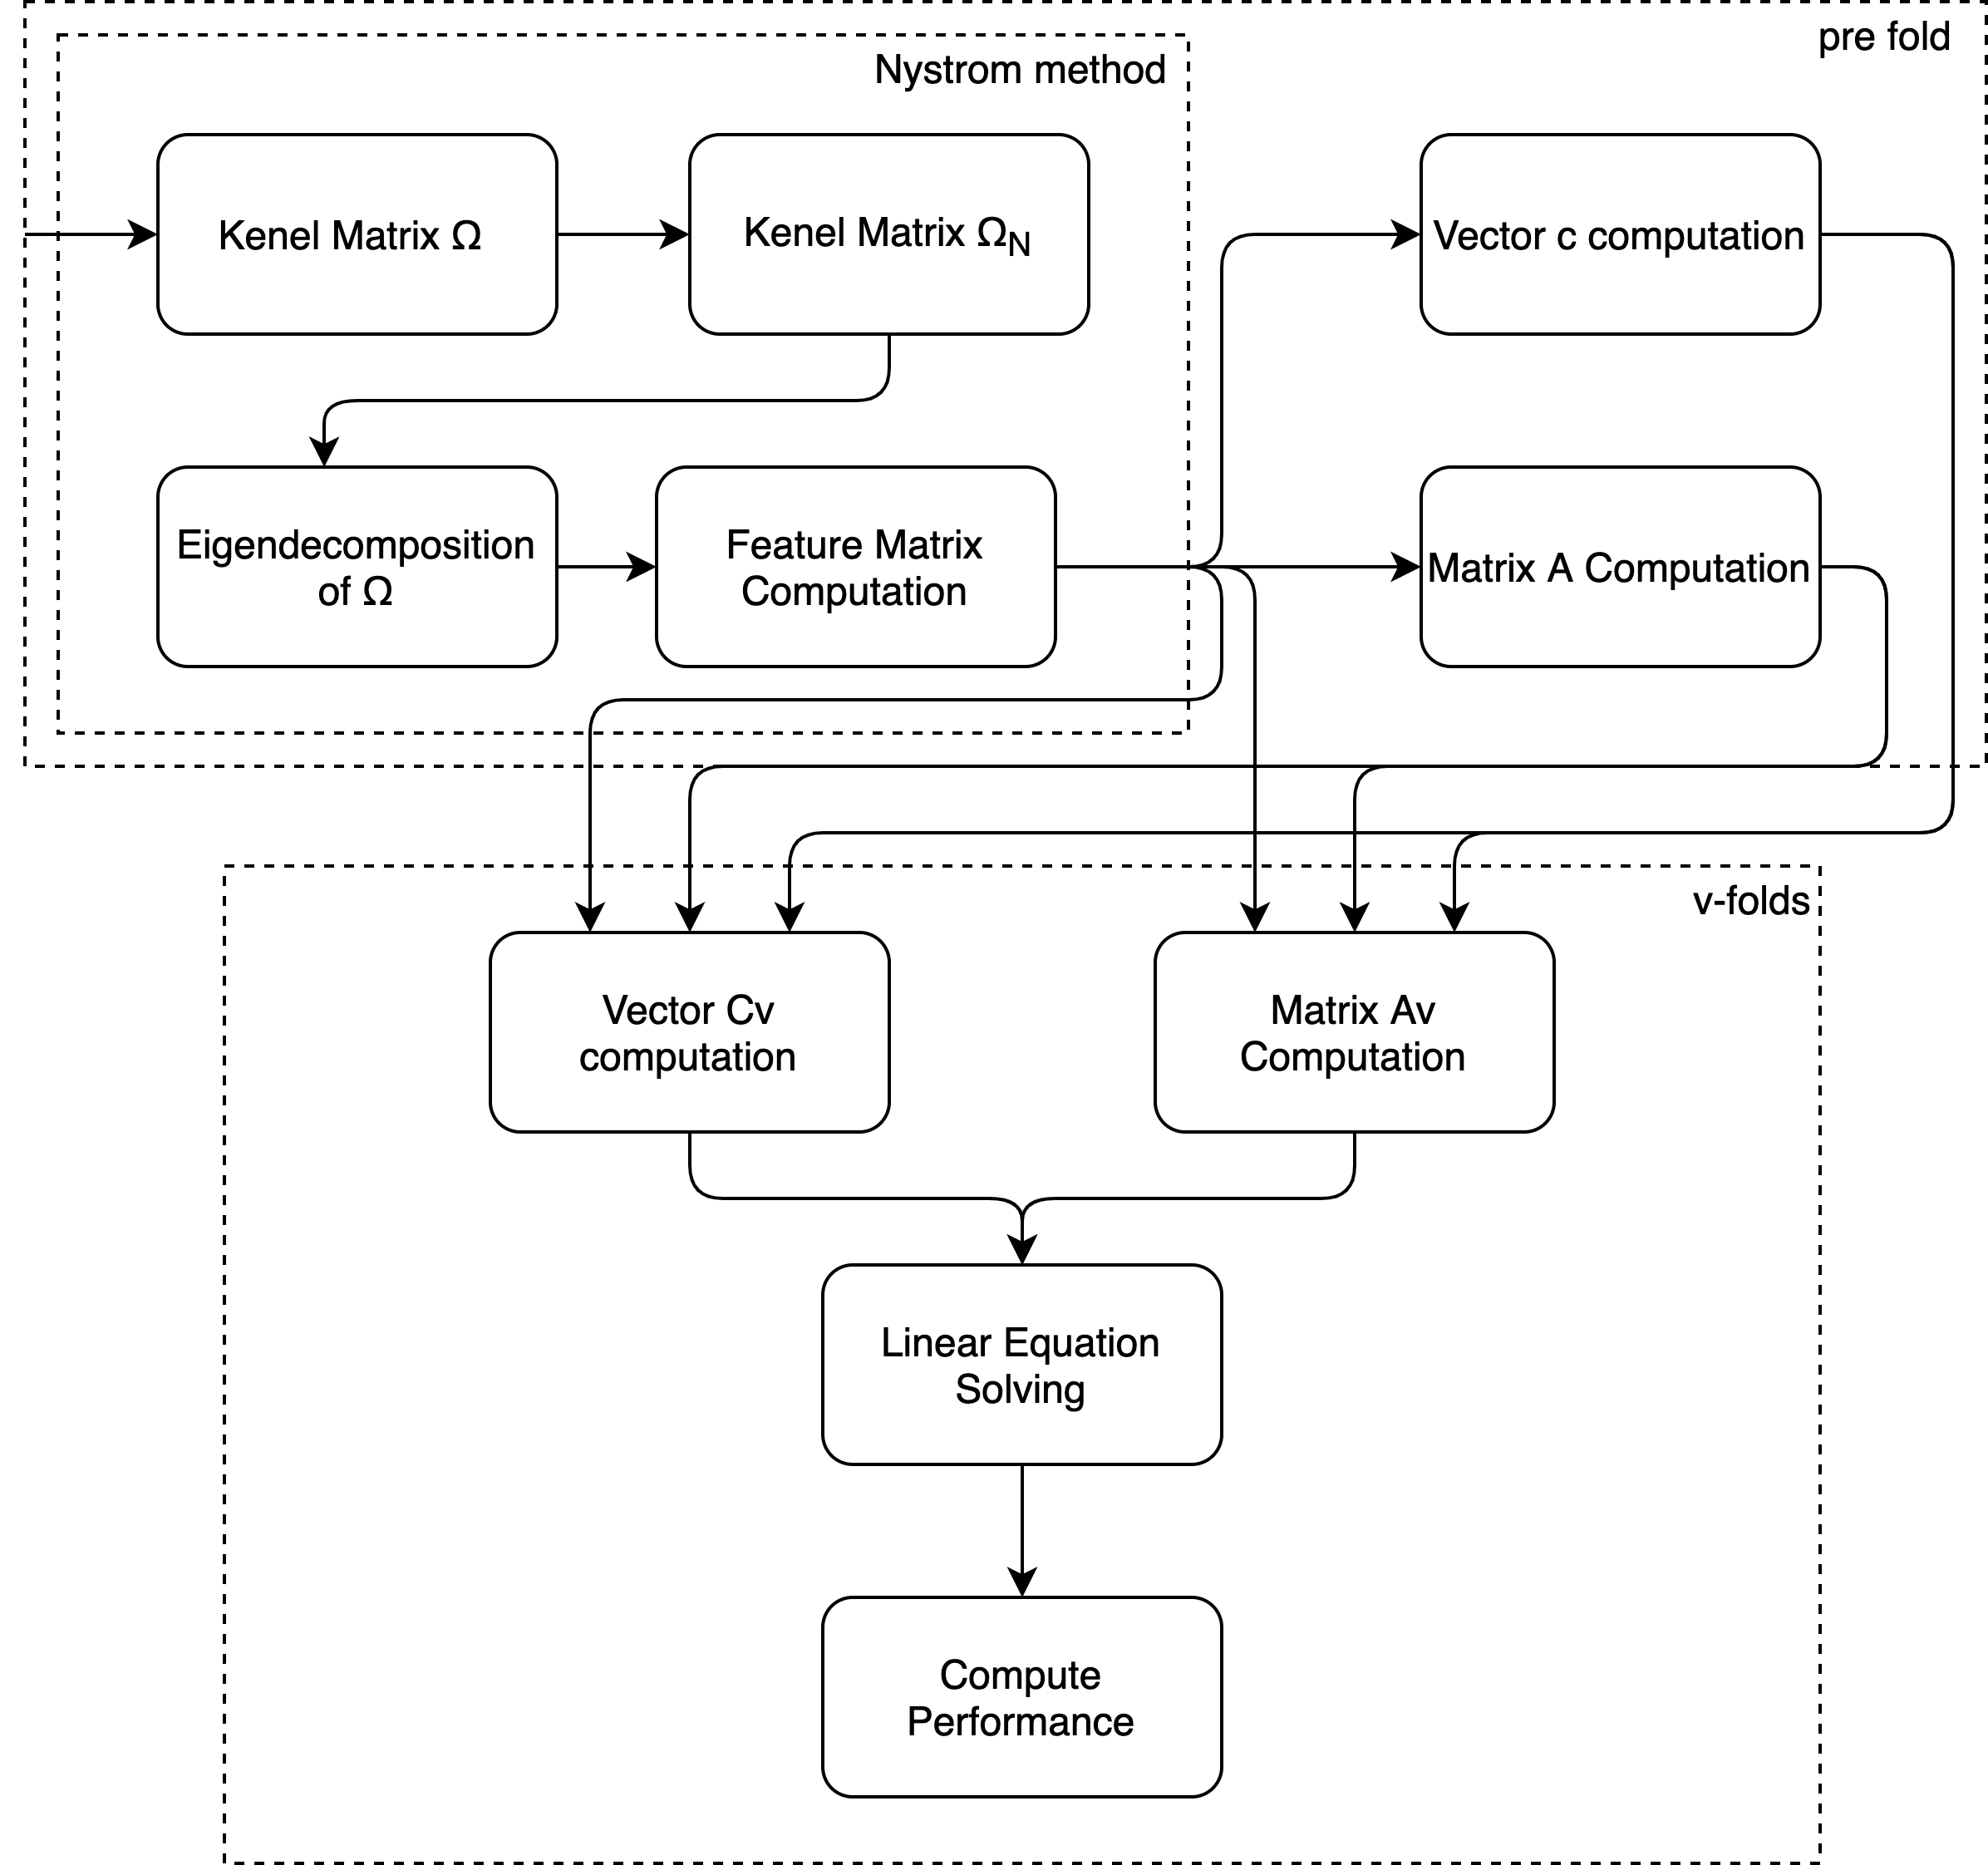
\includegraphics[]{fastvfoldcrossvalidationoverview.png}
	\caption{A detailed overview of the fast $v$-fold crossvalidation algorithm}
	\label{fig:fastvfoldcrossvalidationoverview}
\end{figure}
\subsection{Conclusion}
The Fixed Size Least Square Support Vector Machine algorithm is a variation of the base LS-SVM algorithm.
Designed with large data sets in mind.
The reduction of the amount of support vectors comes however with the introduction of an extra step: the support vector selection.
This together with the tuning of the parameters still asks for some computational power.
Fortunately, a faster cross validation can be used to reduce the amount of computations.\cite{Optimized2010:article}

\section{Parallel computing}
\subsection{Introduction}
In the early decades of computing, parallelism was not a point of attention.
Because of Moore's Law that predicted the amount of transistors in a processor would double every two or so years, the speed-up was mainly focussed on making the CPU faster.
In the late twentieth century, the general interest started to rise. 
Especially after 2004, the turning point for Moore's Law\footnote{The turning point of Moore's law meaning the condition that the amount of transistors would double in a processor every two or so years is not true anymore.}, from then on it was clear that the expectation for speed-up by having more transistors available was in vain.
The course of transistor amount per processor is shown in figure~\ref{fig:Moore}.\cite{rupp_2015}
To be fair, after 2004 CPU's continued on getting better and faster but by optimising other cases rather than the number of transistors. \footnote{Optimization in placement, use of more chache levels, drops in power consumption,....}
\begin{figure}[H]
	\centering
	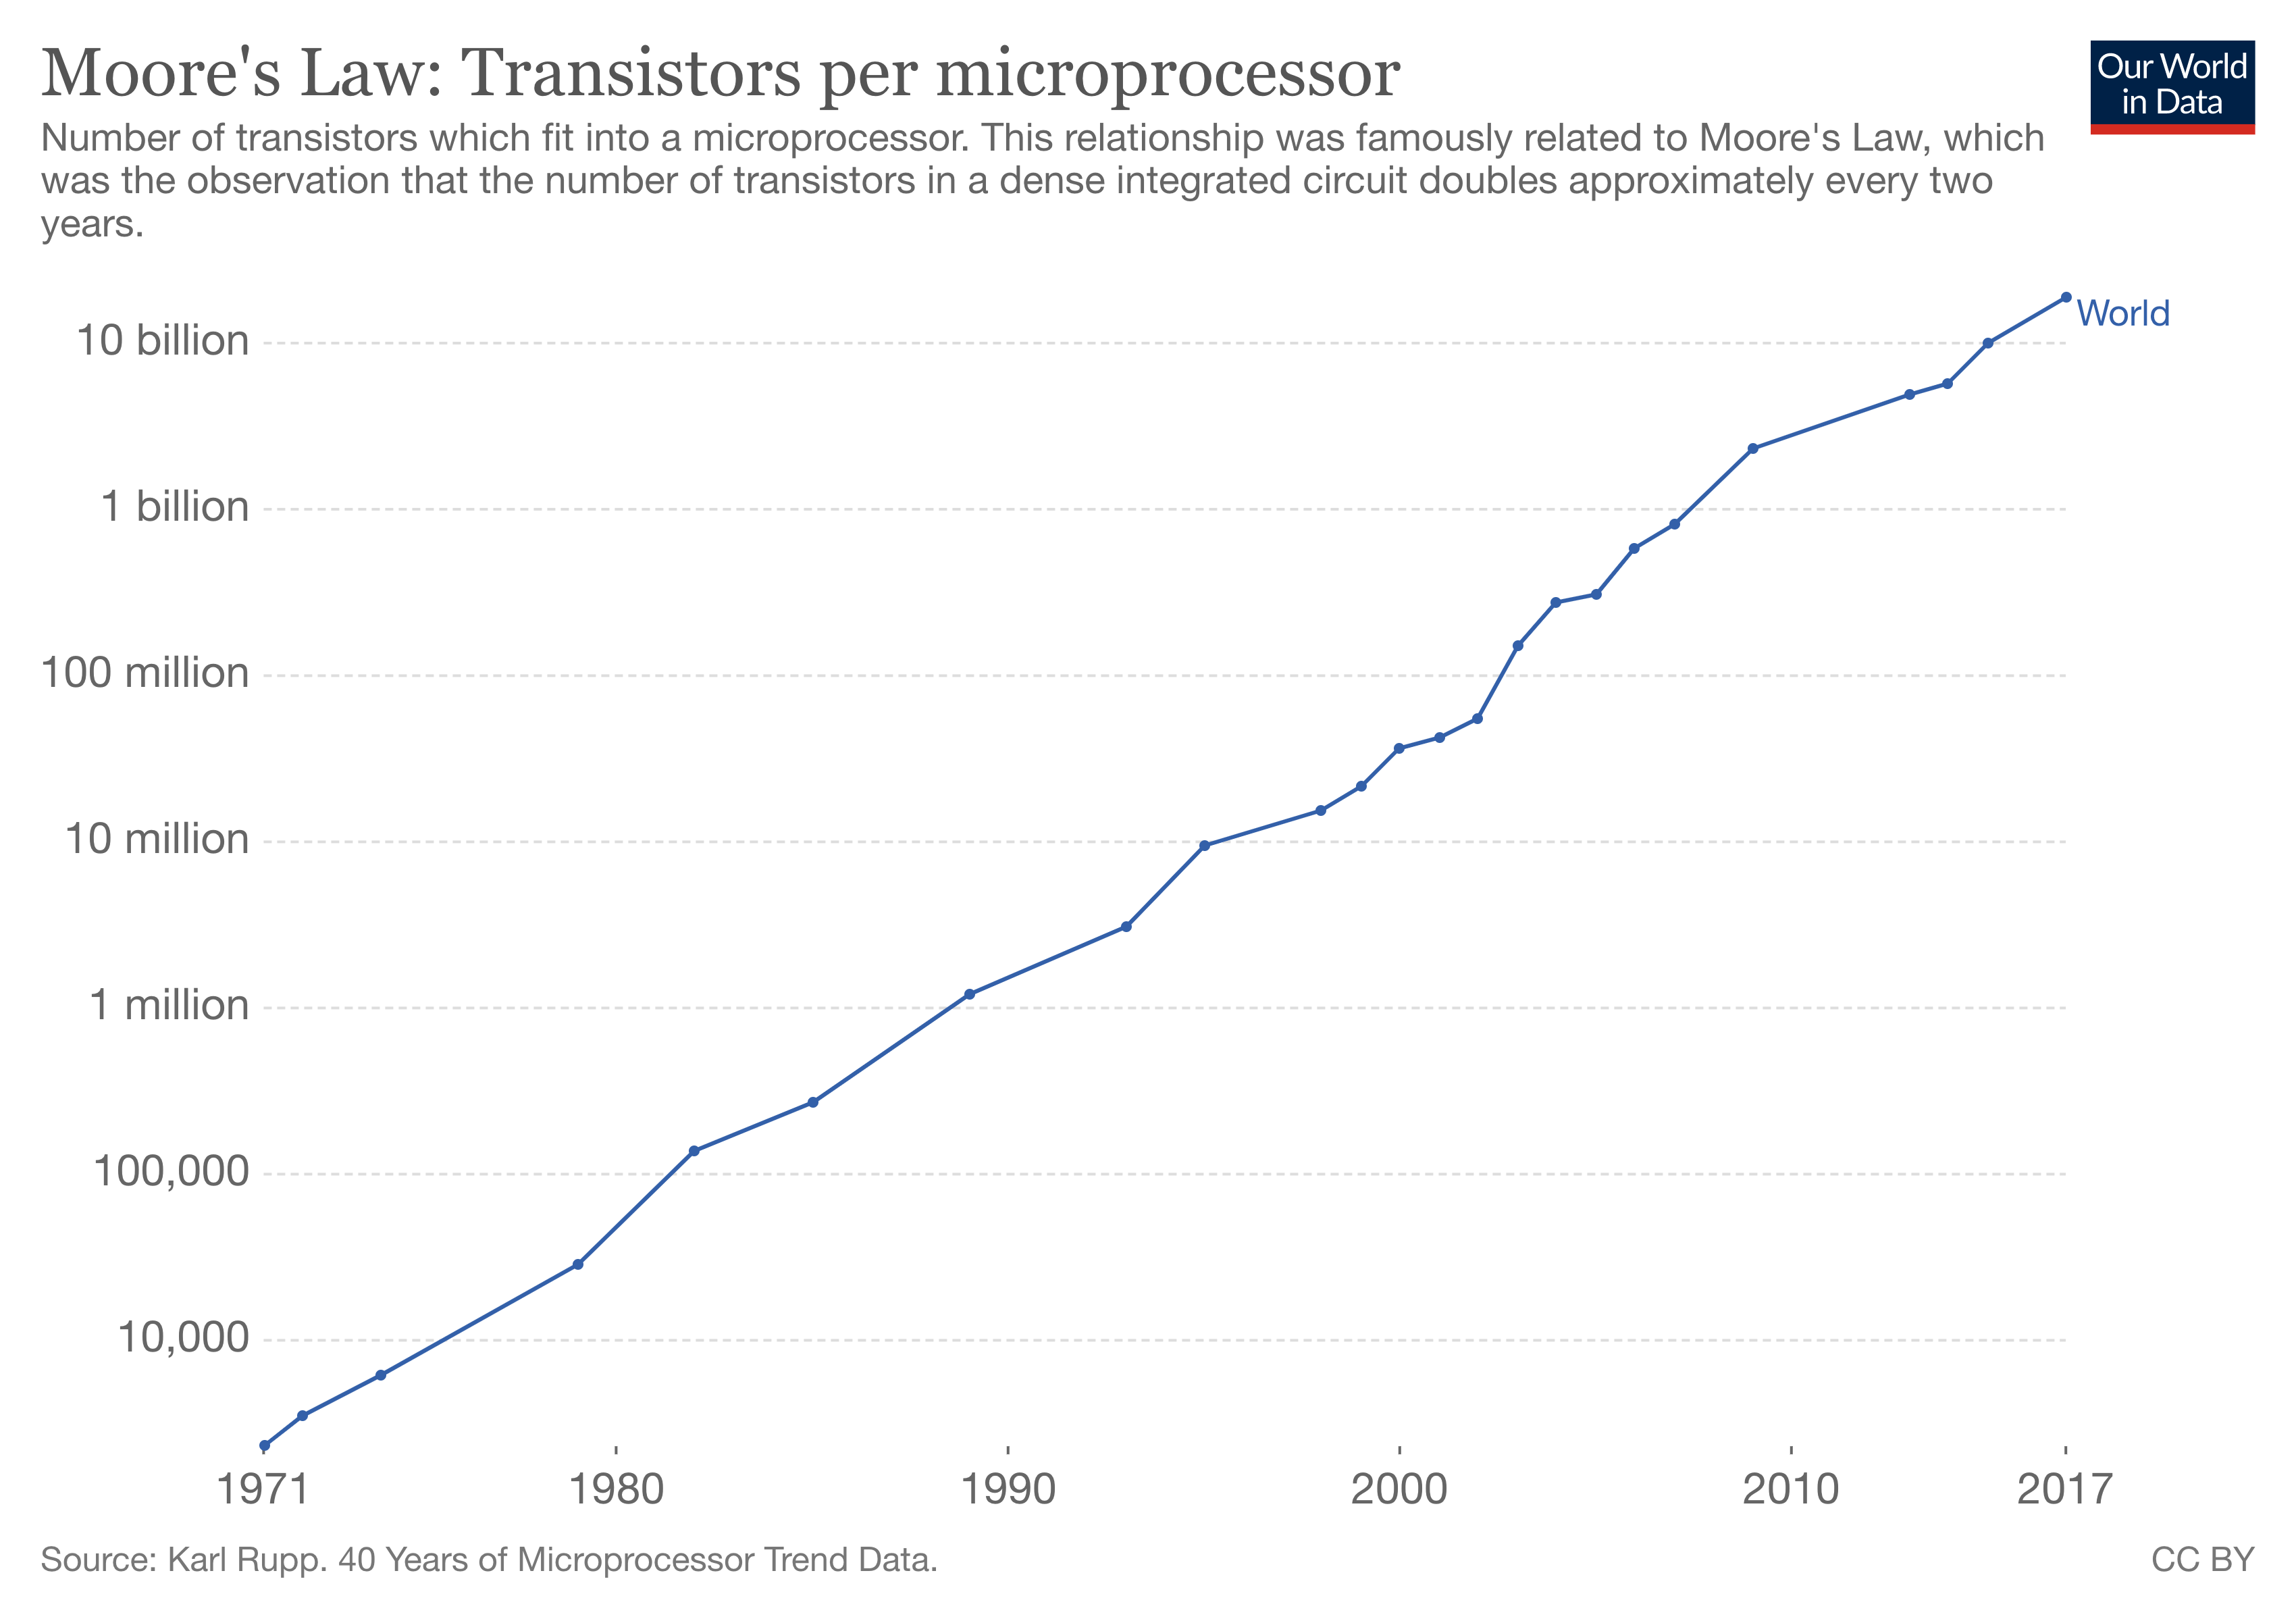
\includegraphics[width=0.8\linewidth]{transistorsPerMicroprocessor.png}
	\caption{Number of transistor per microprocessor.\cite{rupp_2015}}
	\label{fig:Moore}
\end{figure}
The idea behind parallelism is straight forward, where a sequential program is executed on a single processor, in a single stream of instructions, in parallel execution multiple streams of instructions and multiple processors are used.
By channeling program instructions to multiple streams the goal of reducing total executing time can be set.\\
In simple terms one could state that code optimized for parallel execution can reach a speed up factor equal to the number of processors used.
As Amdahl stated, this will never be possible, for the following reasons:
\begin{itemize}
	\item Code is often not 100\% parallel executable, portions of the code will still be serial executed.
	\item Overhead, working with multiple processors (and threads) will create overhead that has to be handled with.
\end{itemize}
Amadahl himself was not a big fan of moving all programs to parallel execution.
He was not opposed against the use of parallel computing but he wanted to state the true speed up and in this way show the science community that code would not magically speed up just by using more processors.
In the case of super scaling the solution (heavily increasing the number of processors), the terms hard scaling and soft scaling are important to keep in mind.
Hard scaling focusses only on the number of processors used to execute a particular block of code, the work done by each processor will be a fraction of the total work.
From a certain moment, the number of available processors will exceed the number of available fractions of work, ramping up the amount of processors will not benefit the speed-up factor what so ever.
Soft scaling uses both the maximum amount of parallelizable and the available processors as an input for Speed Up factor calculations, as shown in equation~\ref{eq:amadahl}.
  
\begin{equation}
	SpeedUp(P,N) = \frac{T_P}{T_S} = \frac{T_S}{\alpha(N) + \frac{(1-\alpha(N))}{P} T_S}
	\label{eq:amadahl}
\end{equation}
with
\begin{itemize}
	\item \textbf{P:} Number of processors.
	\item \textbf{N:} Number of tasks parallelizable.
	\item \textbf{$T_S$:} Execution time when run in serial.
	\item \textbf{$T_P$:} Execution time when run in parallel.
	\item \textbf{$\alpha$:} Function computing the fraction of the code executing in serial.
\end{itemize}
The term overhead is loosely touched earlier in this section, it is a vague term consisting of multiple items.
Overhead can refer to the overhead necessary to create ,and later destroy, threads.
This kind of overhead is predictable because it is only depended on the number of threads that needs to be created and is shown in figure~\ref{fig:forkjoin}.
\begin{figure}
	\centering
	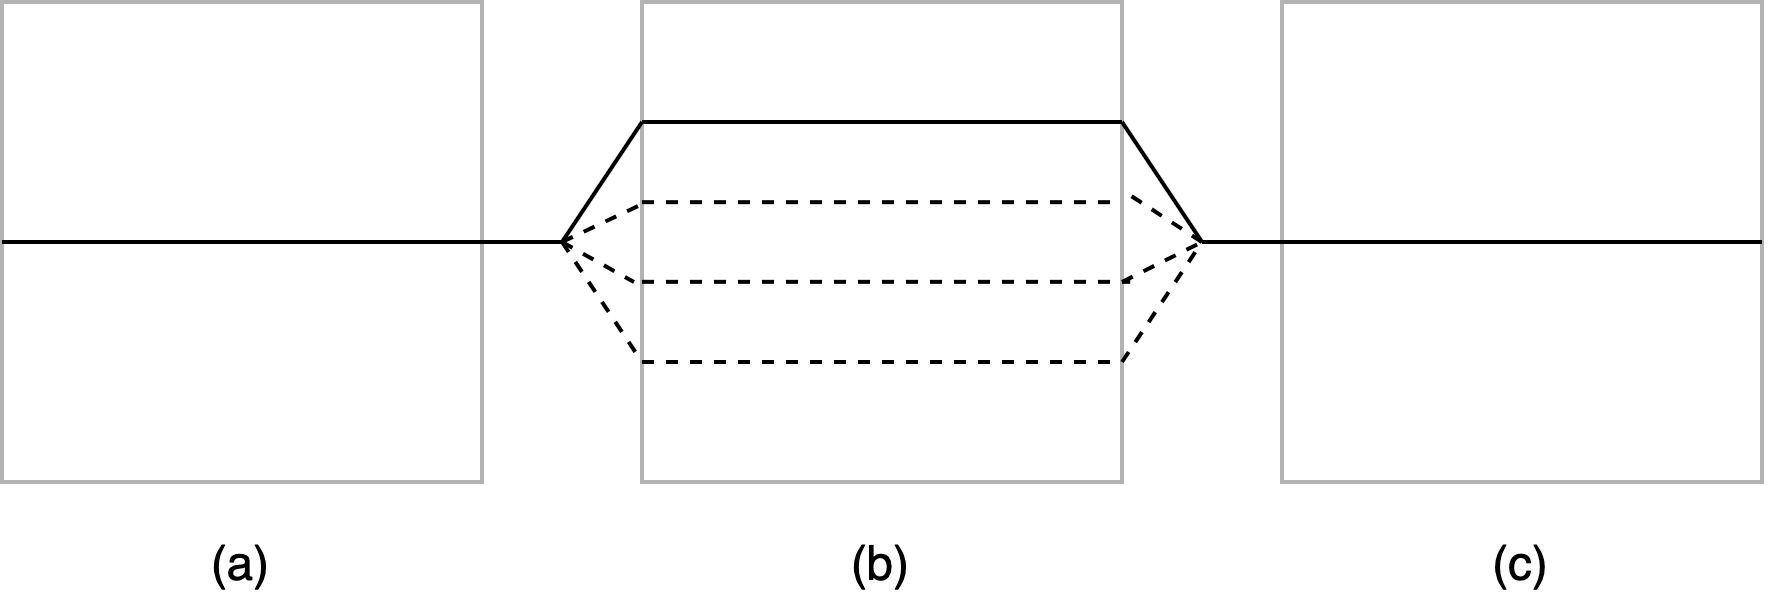
\includegraphics[width=0.8\linewidth]{ForkJoin.png}
	\caption{Thread Fork Join principle. In (a) only the main thread is executing a stream of instructions. In (b) the main thread forked into multiple threads, multiple streams are available here. In (c) the main thread terminated the other threads and joined them back into itself.}
	\label{fig:forkjoin}
\end{figure}
\begin{figure}
	\centering
	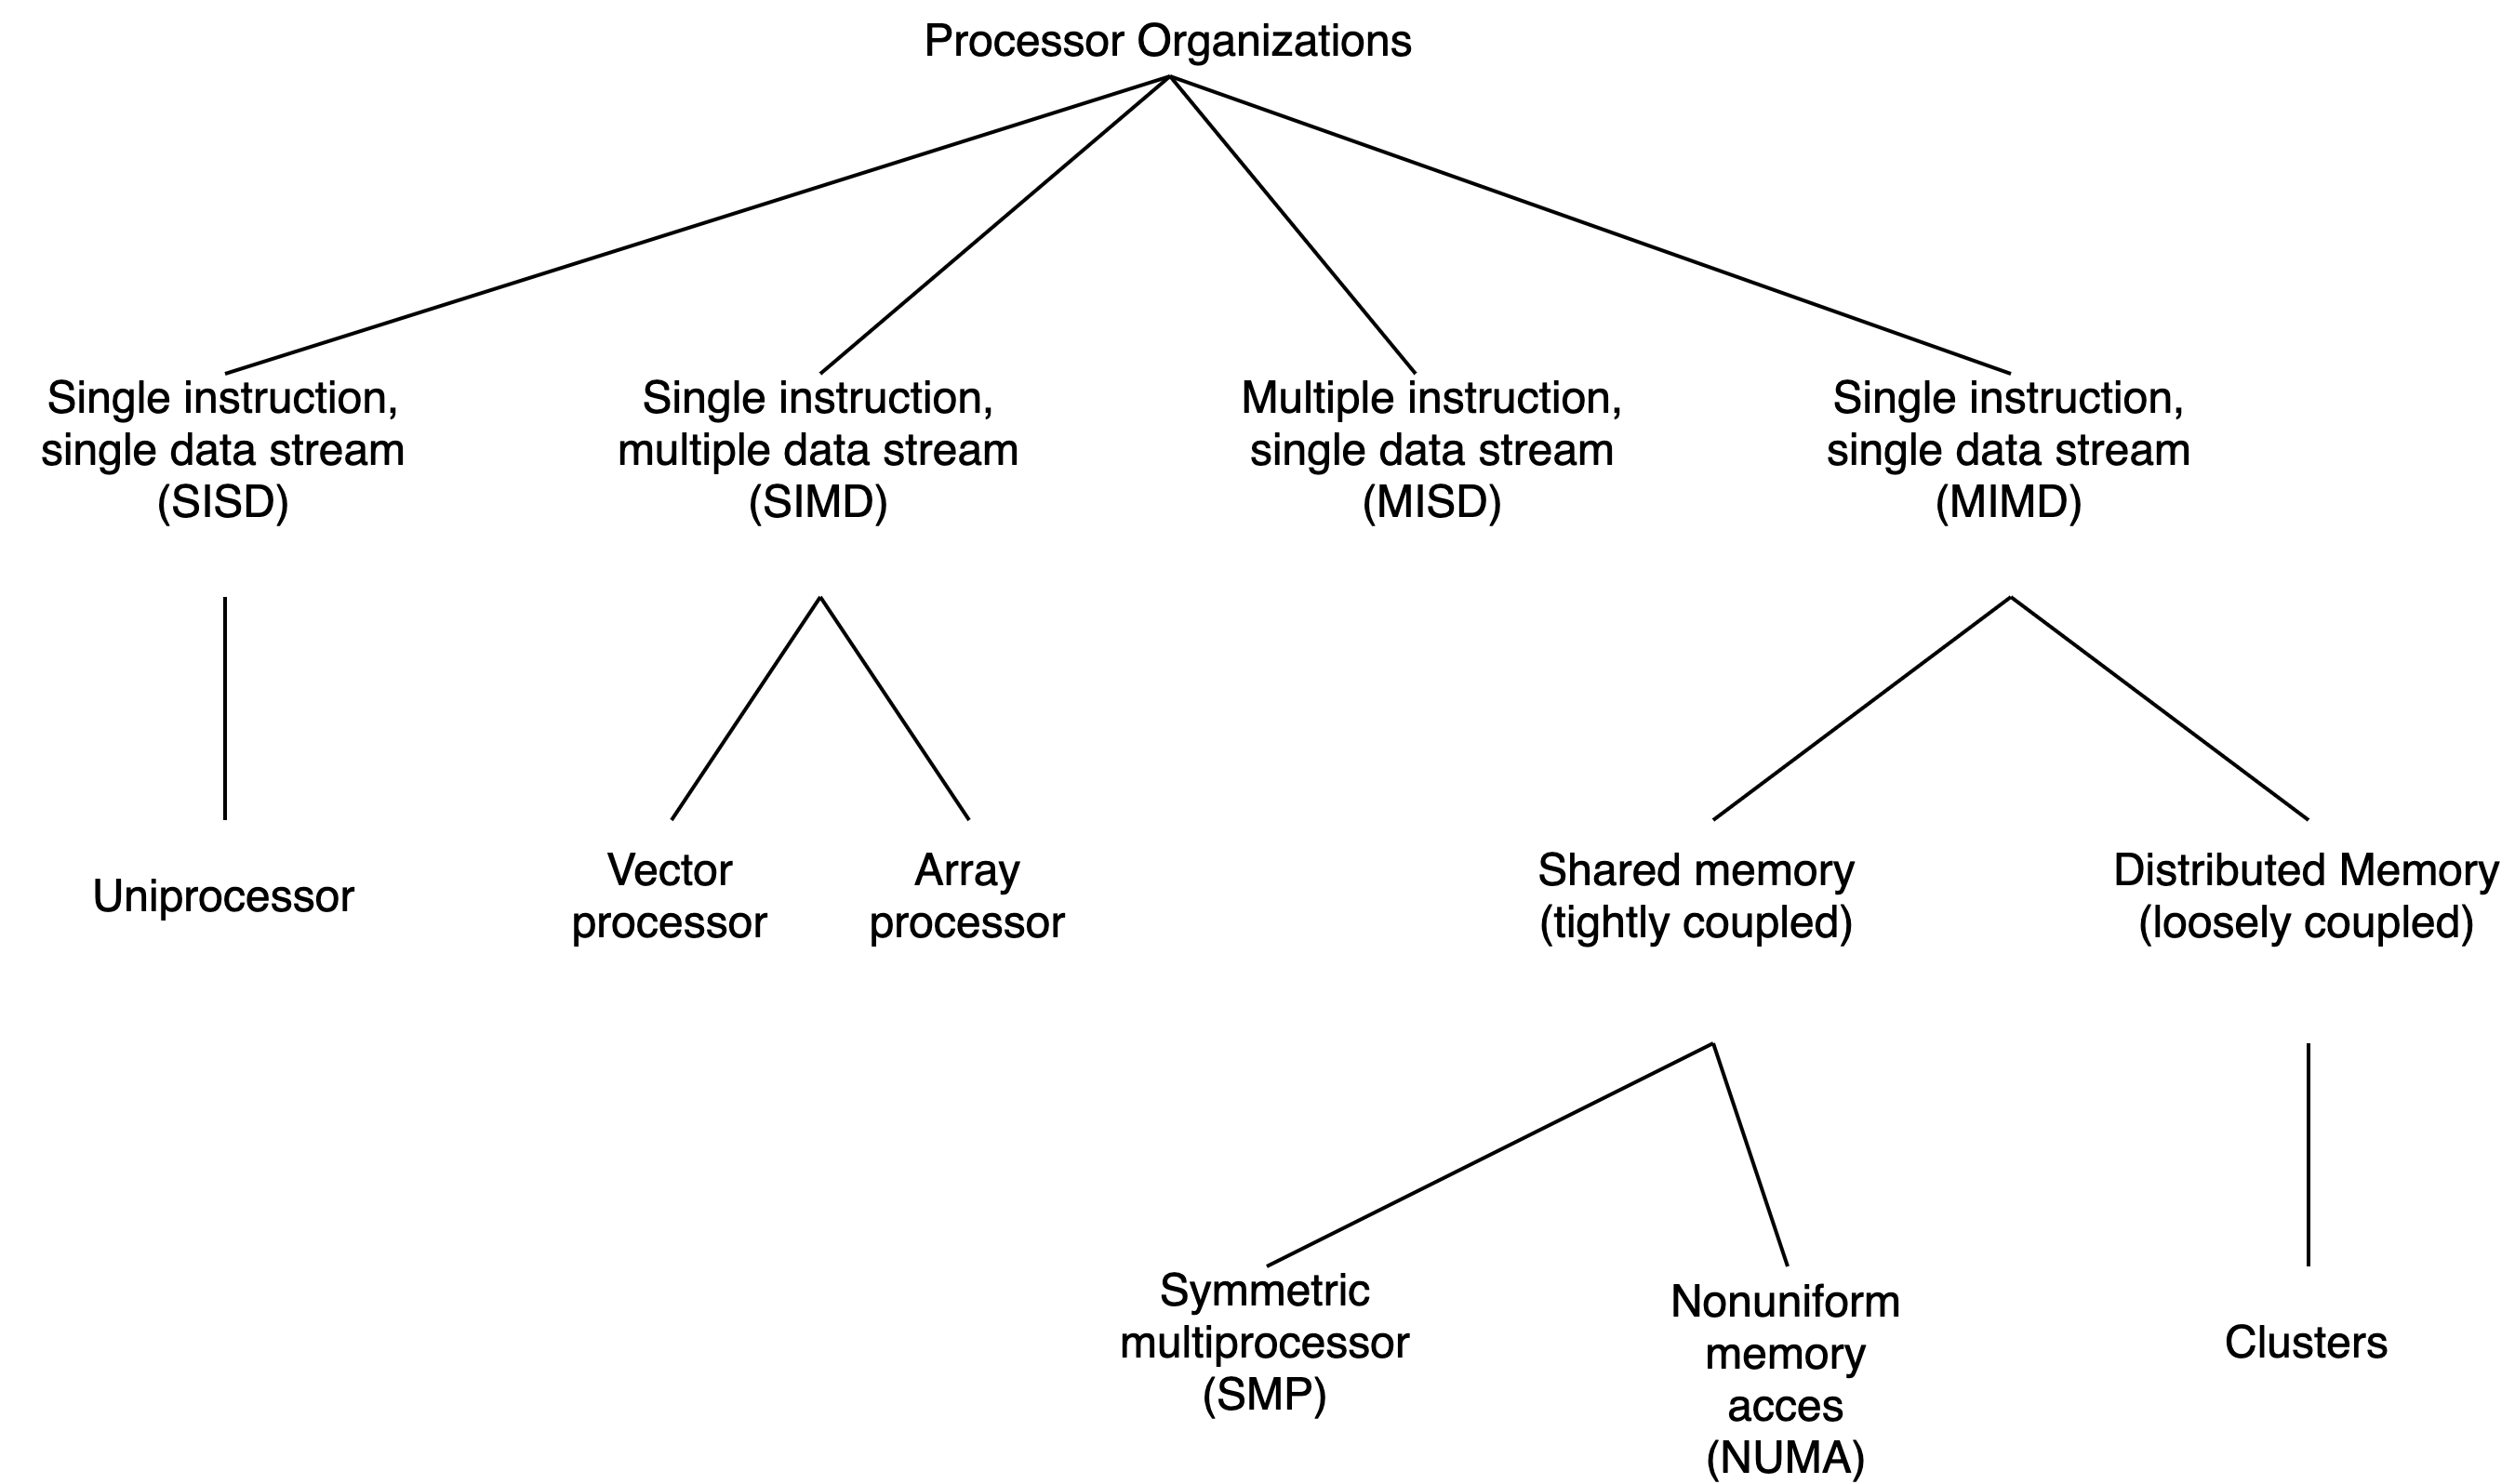
\includegraphics[width=0.8\linewidth]{Parallel_Organizations.png}
	\caption{A Taxonomy of Parallel Processor Architectures as designed by William Stallings.}
	\label{fig:procOrg}
\end{figure}
Memory overhead has to do with all the data being available in memory for the correct processor at the correct time.
In the world of parallel computing this memory management is way more difficult compared to serial computing and is highly depended on the used architecture and memory structure.\\
William Stallings makes an overview of the different processor organizations, as shown in figure~\ref{fig:procOrg}
These are all high level descriptions of parallel computing terms.
Diving in to more details is difficult because it is depended on the way parallel computing is implemented.
Many options are available, as shown in figure~\ref{fig:procOrg} and those all differ in the use of memory management as well as the use of threads and processors.
\par 
The remaining part of this section is focused on the two most common (multi) processor organizations. 
\begin{itemize}
	\item Single Instruction Multiple Data streams (SIMD), or the GPU way with focus on CUDA enabled systems.
	\item Multiple Instruction Multiple Data streams (MIMD), multiprocessor system with scalability 
\end{itemize}
\subsection{SIMD and The World of CUDA}
\subsubsection{Introduction}
Single Instruction Multiple Data stream processors.
This means that a single instruction will be executed on data coming from multiple streams.
Looking at the architecture this means that there will be one control unit\footnote{The control unit is one of the elements of a processor. Processor architecture and organization falls outside the scope of this thesis, however in general a processor consists of the control unit, cache and an Arithmetic Logic Unit. } combined with a cache element, controlling multiple Arithmetic Logic Units (ALU)\footnote{An Arithmetic Logic Unit is the element in a processor where the instructions are effectively executed.}.
A graphic representation of this architecture is shown in figure~\ref{fig:simd}.
\par 
\begin{figure}
	\centering
	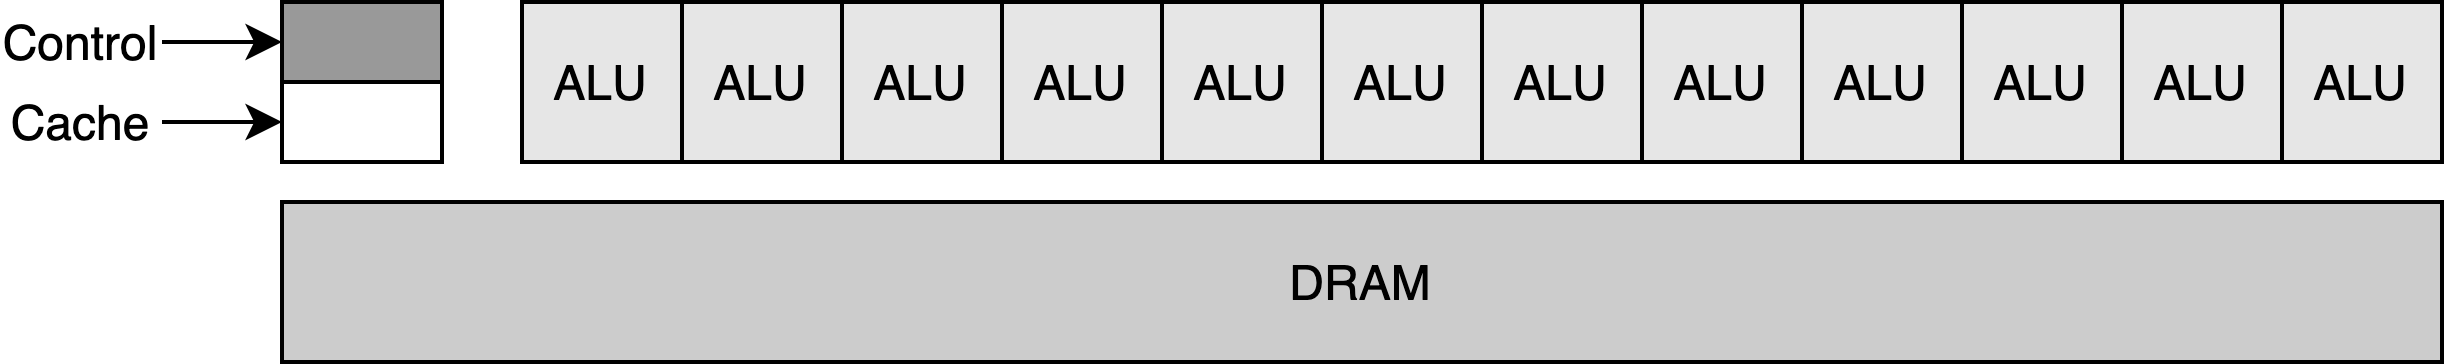
\includegraphics[width=0.8\linewidth]{SIMD.png}
	\caption{A graphic representation of the SIMD architecture.}
	\label{fig:simd}
\end{figure}
The SIMD processors are developed for a certain kind of Instructions and a certain kind of data, meaning the category of instructions that always have to be executed on a large number of data entries.
In reality these are almost always linear algebraic and matrix operations.
Where the same instruction (for example multiplication by a scalar) is executed on all the elements of a matrix.
These kind of mathematical computations are used in complete range of cases. 
Signal processing, video converting, rendering, math calculations, and many more.
Much of those cases are handled by a Graphical Processing Unit (\textbf{GPU}). 
A GPU uses the basic principles of an SIMP architecture, but expands the concept by adding multiple control units.
The idea is shown in figure~\ref{fig:gpu}.
Where multiple control units with dedicated cache each control a number of ALUs.
The logic behind the architecture can be described as combining multiple SIMD processors into a single architecture.
\begin{figure}
	\centering
	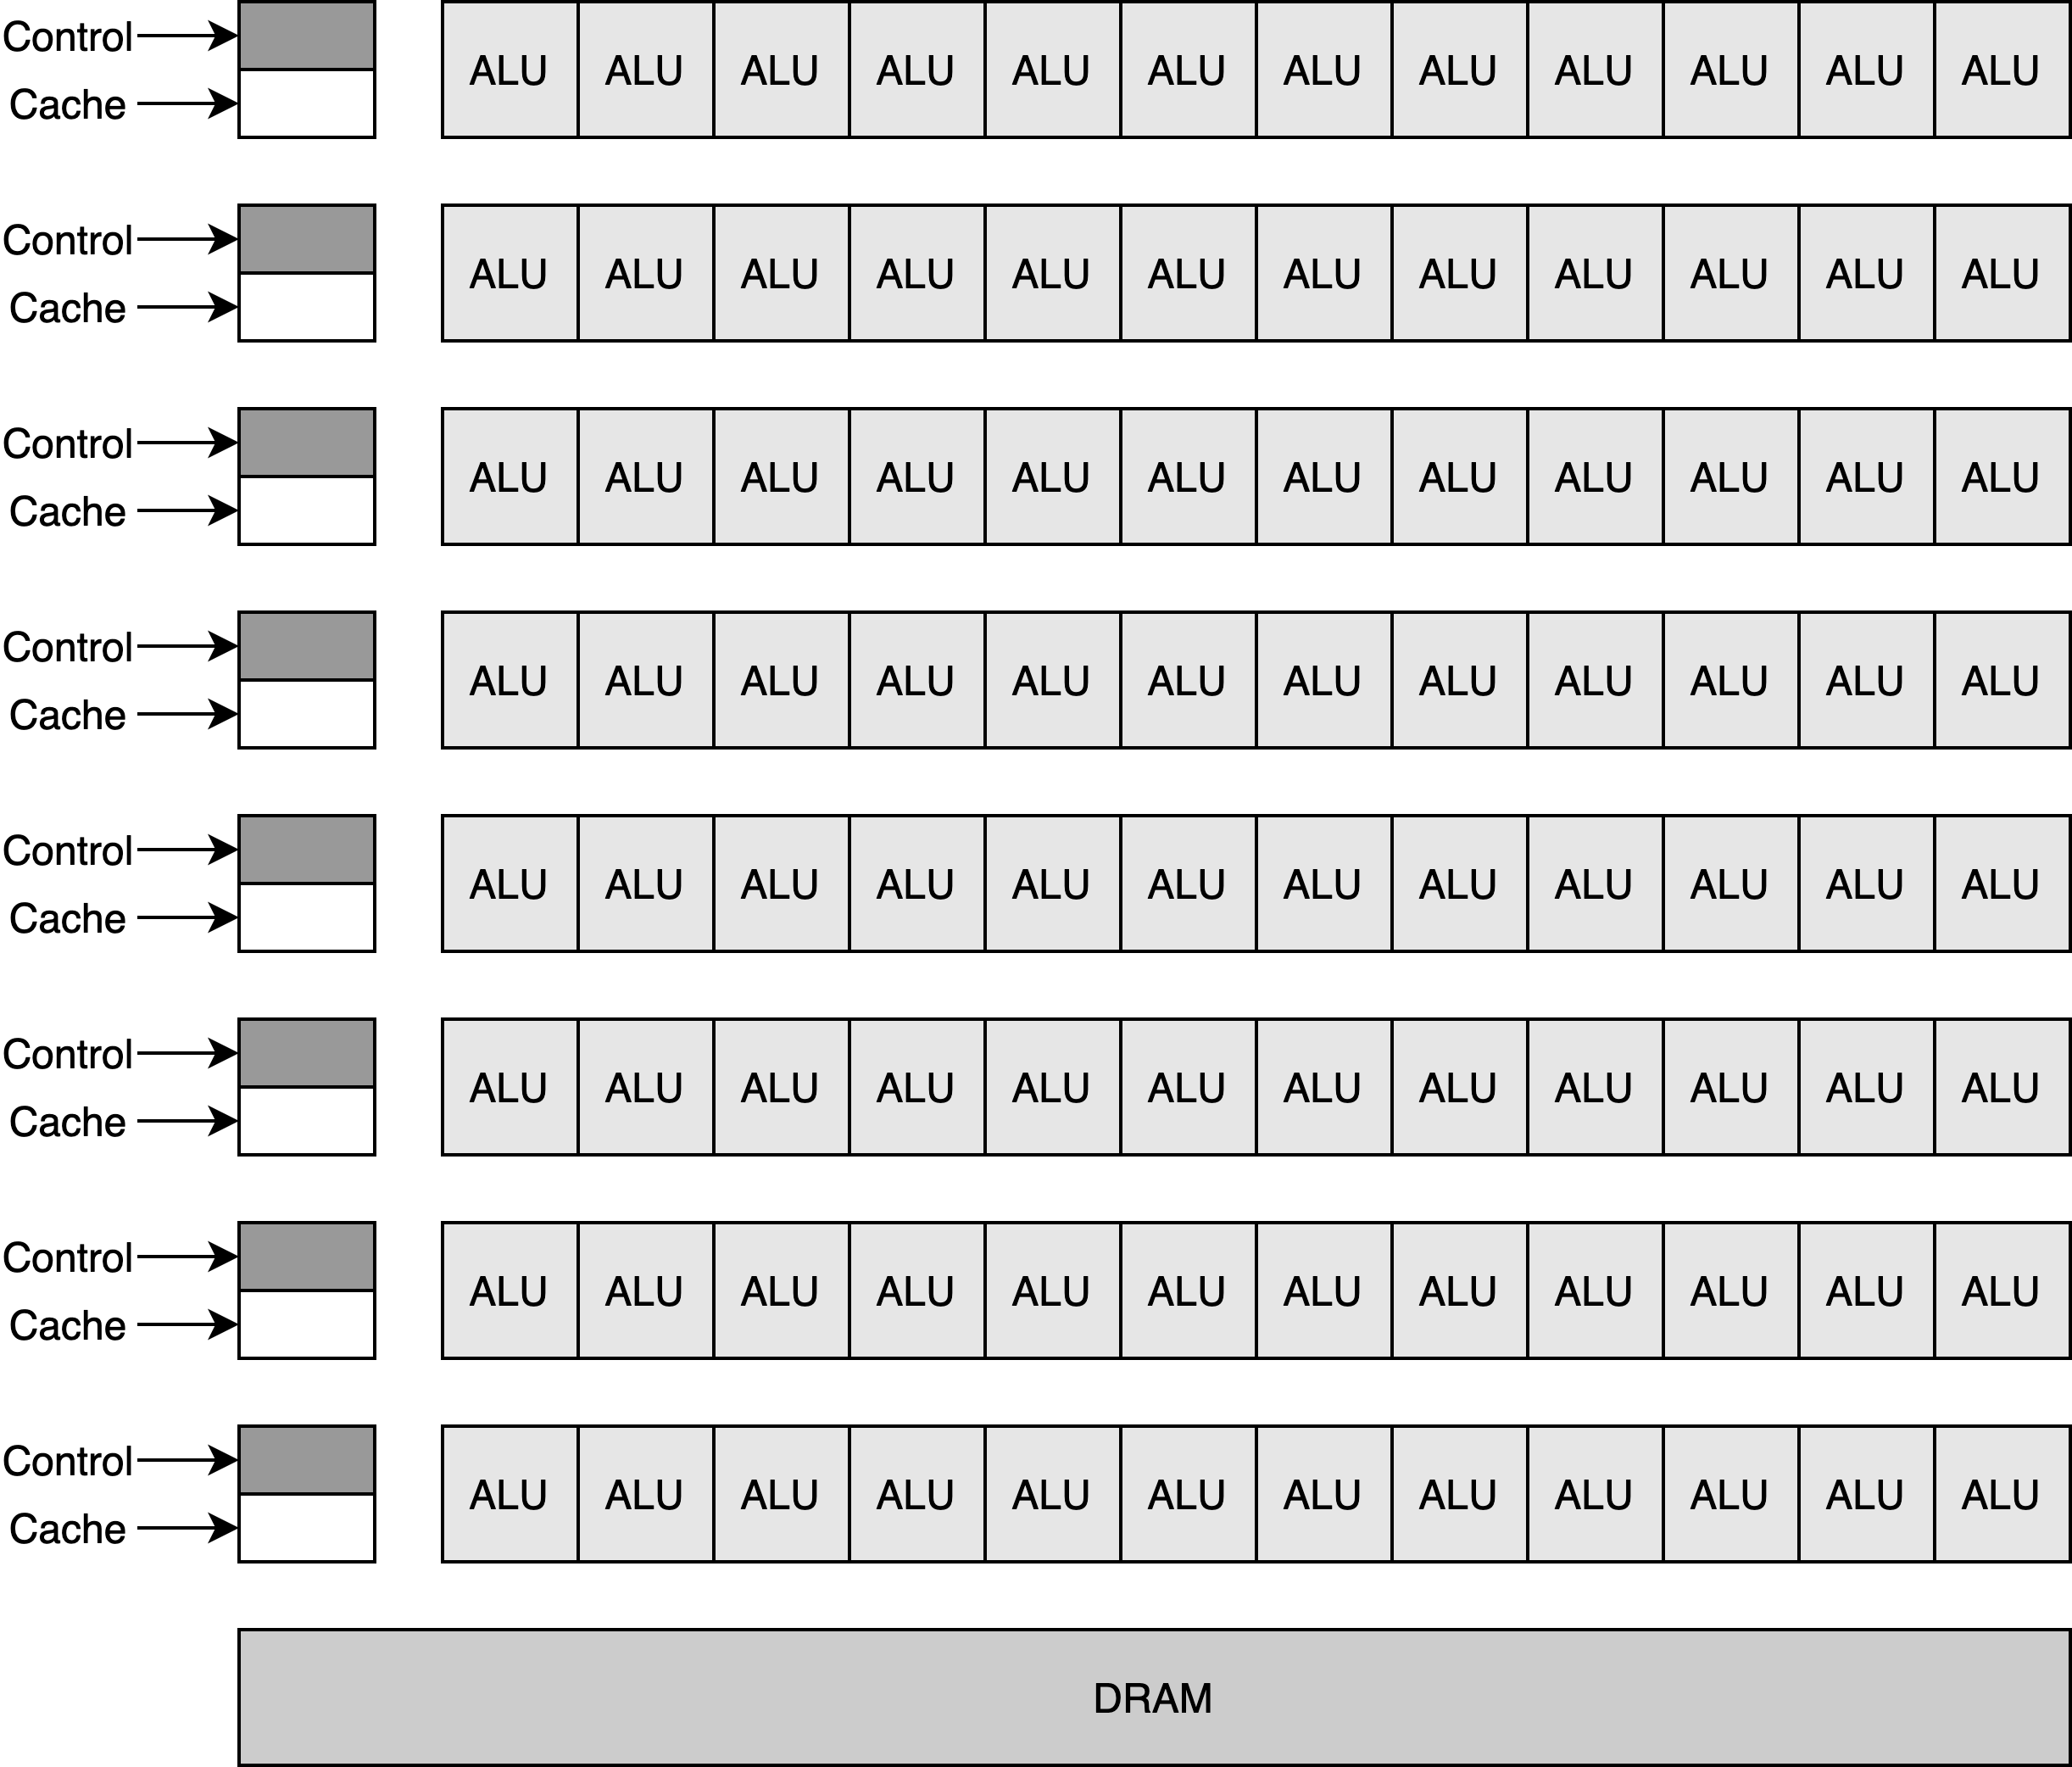
\includegraphics[width=0.8\linewidth]{GPU.png}
	\caption{A graphic representation of a GPU architecture.}
	\label{fig:gpu}
\end{figure}
Figure~\ref{fig:gpu} shows an abstract idea of a GPU, in practice every company that produces GPUs has its own specific implementation or even multiple depending on every model.
\subsubsection{Nvidia and the world of CUDA.}
Well known companies that produce GPUs are NVidia, AMD and Intel. 
To run code and computations on those GPUs, the correct APIs and frameworks are needed.
Those frameworks all have different focus points:
\begin{itemize}
	\item \textbf{Open Graphics Library (OpenGL)}: cross platform framework for rendering 2D and 3D vector graphics.
	\item \textbf{DirectX}: Windows (and Xbox) framework for accelerating video decoding.
	\item \textbf{Mantle}: AMD GPU specific rendering API targeting 3D video games.
	\item \textbf{Vulkan}: cross platform low overhead 3D graphics API.
	\item And many, many more.
\end{itemize}
The frameworks (and or APIs) have a list of specific hardware models they support and on which platform they the software can run.
As well as those limitations, each framework has his own specific language to control the GPU.
\par 
NVidia developped a separate API for their GPU range, not with specific use cases in mind, but based on well known languages and with giving developpers in an easy way maximum control.
This API is called \textbf{CUDA} (Compute Unified Device Architecture) and is freely available.
CUDA language is very similar to C/C++\footnote{CUDA fortran is a variation working with FORTRAN code.} and can, with the correct compiler installed, execute code from your C program on the (Nvidia) GPU.
Besides the native support for C/C++ and Fortran, third party wrappers exist to make code from a whole range of languages work with the CUDA API, including Python, Perl, Java, Ruby, Matlab...
Although Matlab parallel toolbox also provides native support for CUDA utilization.
Over the years many very reliable libraries are created to execute most kind of linear algebraic computations as well as video coding.
\begin{itemize}
	\item \textbf{AMGx}: Algebraic Multi-Grid
	\item \textbf{cuDNN}: Deep Neural Network
	\item \textbf{cuFFT}: Fast Fourier Transforms
	\item \textbf{cuBLAS}: Basic Linear Algebra Subroutines
	\item \textbf{cuSPARSE}: Sparse Matrix Routines
	\item \textbf{cuSOLVER}: Dense and Sparse Direct Solvers
	\item \textbf{cuRAND}: Random Number Generation
	\item \textbf{GRE}: GPU Rest Engine
	\item \textbf{TensorRT}: Deep Learning Inference Engine
	\item \textbf{NPP}: Image \& Video Processing Primitives
	\item \textbf{nvGRAPH}: Graph Analytics library
	\item \textbf{IndeX}: IndeX Framework 
	\item NVIDIA Video Codec Libraries
	\item \textbf{Thrust}: Templated Parallel Algorithms \& Data Structures
	\item CUDA Math Library
\end{itemize}
The CUDA API together with those library offer a solid foundation for anyone wanting to take his software into the parallel computing world.
\par
A typical workflow of CUDA code consists of the following.
Copying the data from the main memory to the GPU dedicated memory \textbf{(1)}. 
Fetching the instruction from  the CPU to the GPU \textbf{(2)}.
The GPU fetches the needed data from its dedicated memory \textbf{(3)}.
Execution of the code by multiple cores on the data. \textbf{(4)}.
Returning the results to the main memory \textbf{(5)}.
The workflow is shown in figure~\ref{fig:cudaproc}.
This is a possible workflow, however the general principals remain the same.
The CPU will always provide the instruction stream for the GPU.
The memory management can hardly vary depending on the architecture of the system.
\begin{figure}
	\centering
	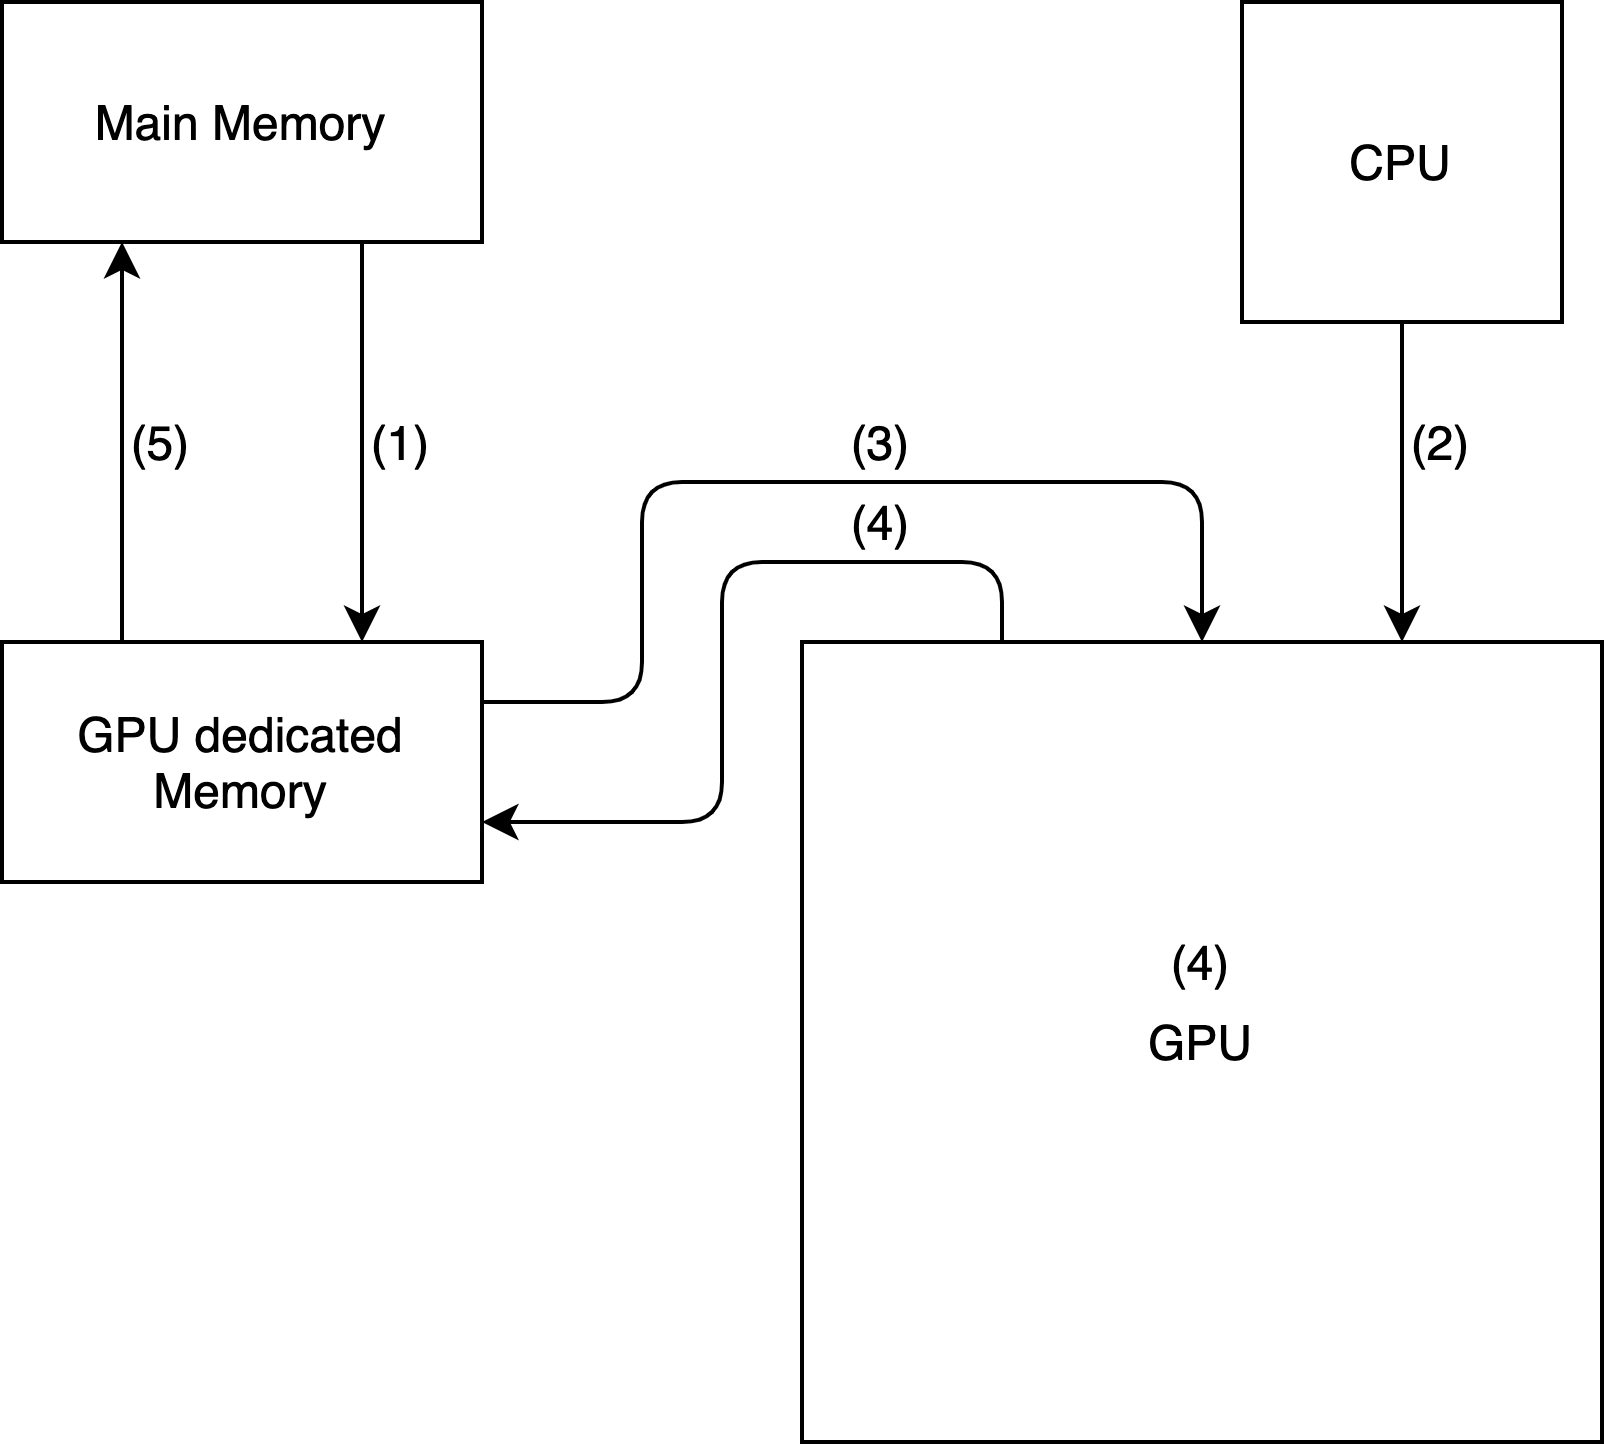
\includegraphics[width=0.8\linewidth]{cudaProces.png}
	\caption{Typical workflow for executing CUDA code.}
	\label{fig:cudaproc}
\end{figure}
\subsubsection{Conclusion}
SIMD forms a basic principle for the GPU design. 
How this design is implemented differs from company to company but basic principles remain.
\par 
CUDA offers a very specific parallelization: all the available cores execute the same instruction.
For matrix operations this is ideal but it is still very specific.
One cannot say fork into $n$ different threads and have them execute different instructions before joining back together, 
which gives the programmer less freedom on how to use it's parallel capabilities.
In other words, CUDA is useful to parallelize the linear algebraic computations of your software.
\par 
The second restriction is the Nvidia brand. 
CUDA is developed, maintained and distributed by Nvidia.
Where it is available free of charge to all who wants, it is restricted in compatibility with Nvidia GPUs only.
Meaning that software parallelized with CUDA becomes hardware platform specific.

\subsection{MIMD: Multiprocessor parallel computing }
\subsubsection{Introduction}
Where SIMD organized processors are considered a custom branch in the processor organization family tree, MIMD organized processors can be considered in the same category as the CPU.
Therefore it is useful to start with a quick update on the main elements of a CPU.
CPU stands for Central Processing Unit and is the processor in most general purpose and personal computer.
Although every model, family from every brand differs in architecture, the general concepts remain the same.
This overview is shown in figure~\ref{fig:cpub}. 
A CPU contains of the following elements:\footnote{The buses coming out of the actual CPU are system busses linking the different elements of the computer system together. For the sake of this diagram and understanding it is enough to think that it 	is just connected to the main memory. }
\begin{itemize}
	\item \textbf{Control Unit}: Unit that control the registers, ALU and control bus.
	\item \textbf{Arithmetic Logic Unit or ALU}: Unit that does the actual execution of an instruction. The ALU is capable of a number of instructions, these instructions are bundled in an instruction set.
	\item \textbf{Registers}: A number of registers that can contain instructions, data, addresses, pointers, counters and buffers for the different buses.
	\item \textbf{Control Bus}: Bus controlled by the control unit to speak with the different connected elements and control them.
	\item \textbf{Address Bus}: Bus used to put on memory addresses, the bandwidth of the bus defines the size of the address space.
	\item \textbf{Data Bus}: Bus used to transfer data to and from the CPU.
\end{itemize}
This organization can be extended with a memory model where fast cache memory or multiple cache memory levels are added.
\par 
\begin{figure}
	\centering
	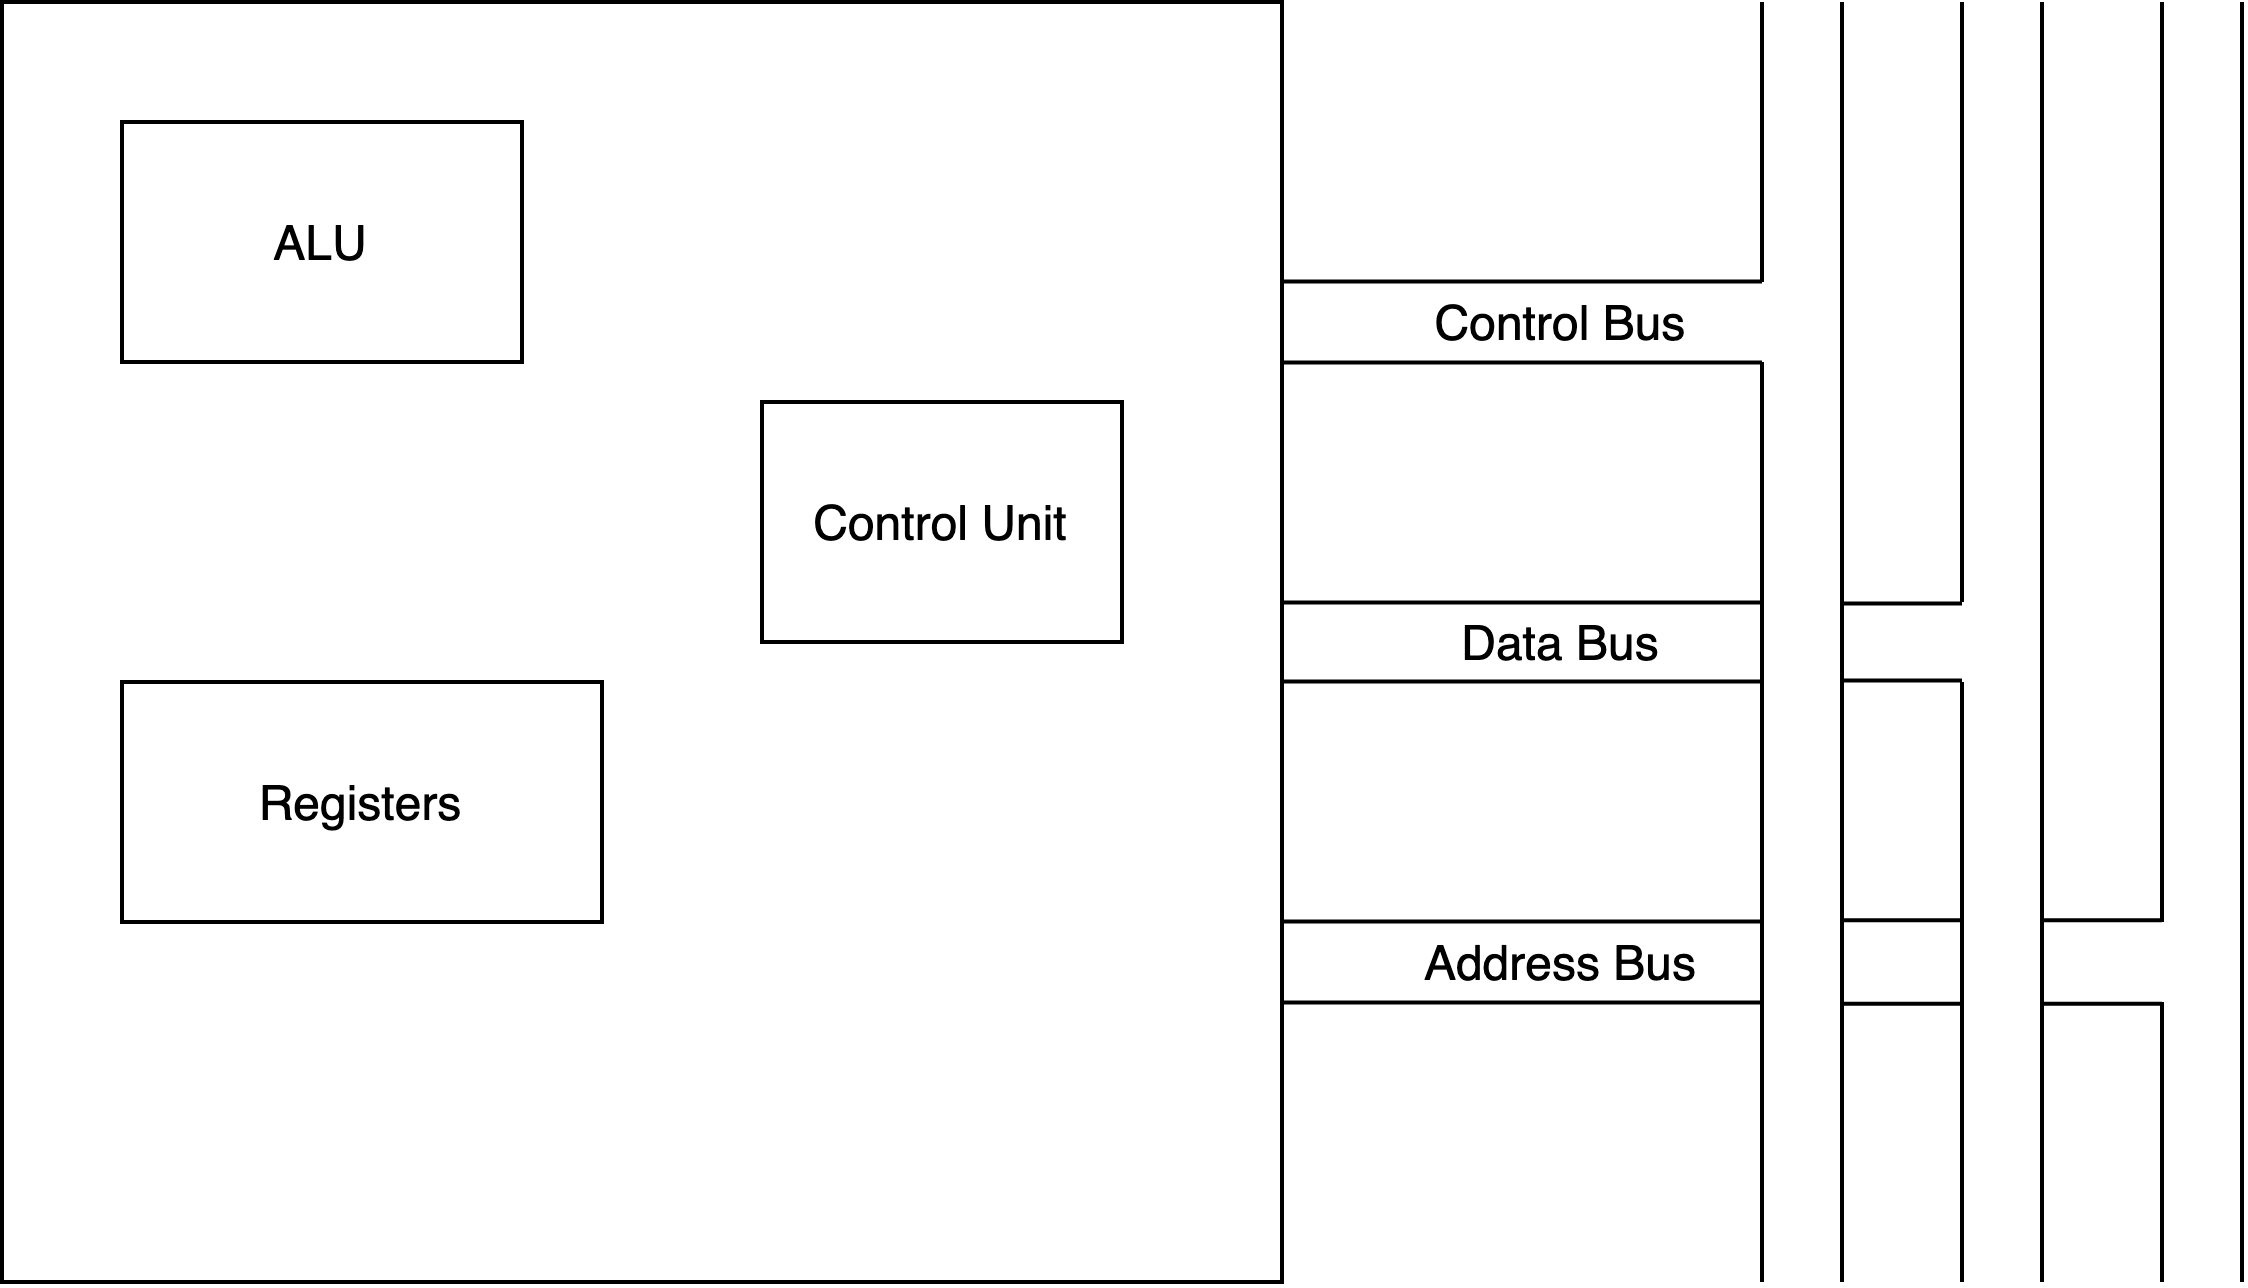
\includegraphics[width=0.8\linewidth]{CPUbasic.png}
	\caption{Basic overview of a CPU}
	\label{fig:cpub}
\end{figure}
With this in mind back to the MIMD organization.
The organization of an MIMD processor organization is shown in figure~\ref{fig:mimdOrg}. 
With \textbf{CU} being a Control Unit, \textbf{PU} a Processor Unit, \textbf{LM} for Local Memory, \textbf{IS} an Instruction Stream and \textbf{DS} a Data Stream.
Figure~\ref{fig:mimdOrg} also shows two possible options for MIMD organizations.
One being a multi processor organization with shared memory and the other being a multi processor organization where the processors are on different systems and share an interconnection network.
\begin{figure}
	\centering
	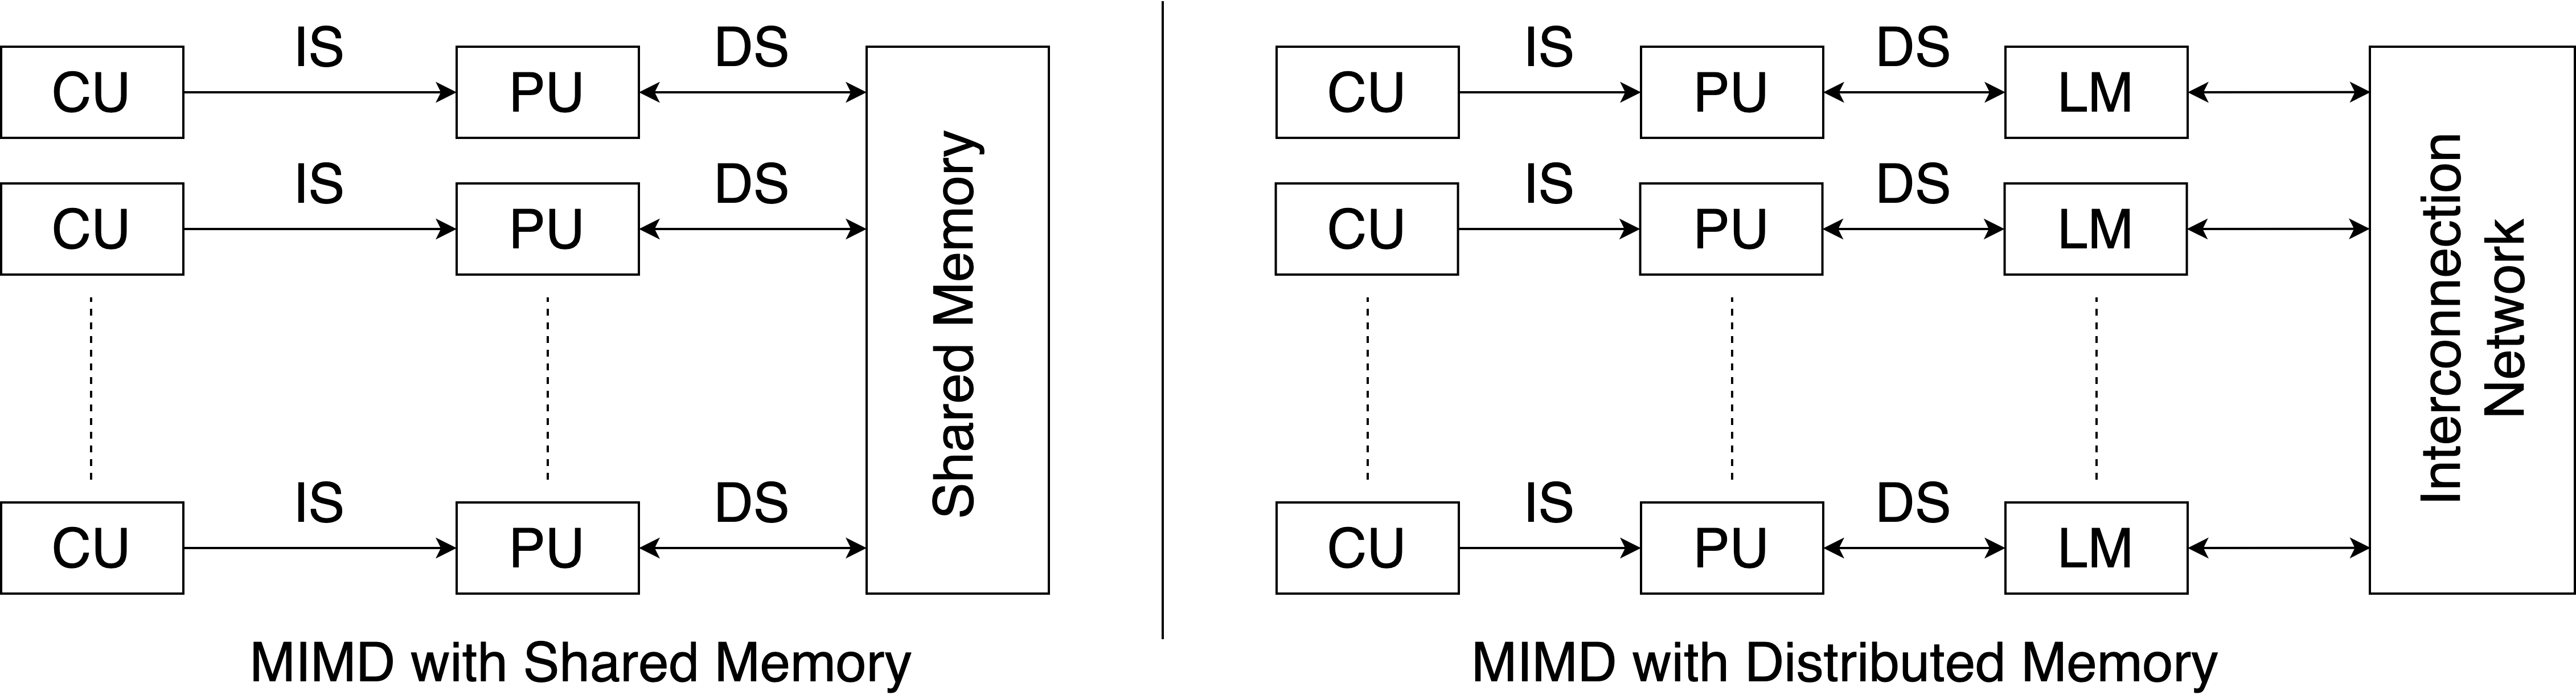
\includegraphics[width=\linewidth]{MIMD_Organization.png}
	\caption{Possible Multiple Instruction Multiple Data stream processor organization.}
	\label{fig:mimdOrg}
\end{figure}
For the scope of this thesis the focus lays on MIMD systems with shared memory organization.
A shown in figure~\ref{fig:procOrg} we can further divide this category into SMP and NUMA organizations.
Again for the scope of this thesis the focus lays on Symmetric multiprocessor organizations (SMP).
\subsubsection{SMP}
SMP organizations can be referred to as stand-alone computer organization with following characteristics:\cite{stallings2016computer}
\begin{itemize}
	\item Two or more similar processors are present.
	\item These processors share the same main memory, I/O facilities and are interconnected.
	\item All processors have equal access to the I/O devices.
	\item All processors posses the same instruction set.\footnote{The instruction set is the collection of all the instructions a processor can execute, usually this is processor model specific.}
	\item The system is controlled by an integrated operating system that utilizes the multiple processors and provides interaction between them in the form if jobs, task threads,....
\end{itemize}
Where symmetric mostly points to item four: all processors are capable of the same operations.
Therefore the operating system can threat the processors as equal.
The organization and development of SMP MIMD processors mostly originates in jumping up the performance of uni processor systems.
Compared to uni processor systems the main advantages are in performance, availability, Incremental growth and scaling.
Where scaling is particularly important in our interest.
\par
An important difference between SMP and the previously described GPU is that every processor has his own Control Unit and cache memory.
How the cache memory is distributed and the amount of levels and size that is used depends on the manufacturer.
Because of that every processor in the system is addressable, giving the operating system more freedom compared to the GPU.\footnote{The upsides of the GPU are widely discussed previously.}
The operating system utilize the system to execute different instructions at the same time.
However this introduces design concerns not present in th GPU.
Because every processor has dedicated cache memory, race conditions can occur and concurrency problems make an entrance.
When a processor does an operation on a certain block of data and that data is possibly needed for other instructions, one has to be sure that the data has the correct value before executing.\\
Memory persistence creates more overhead what limits the speedup factor.
Ideal the multiple instruction streams operate completely independent from each other and do not use the same data blocks.
This ideal situation is never reached so overhead operations will always occur.
\par 
In general this organization gives the programmer and/or operating system a higher grade in flexibility but it comes at the cost of more complex scheduling, synchronization and memory management.
These are also things programmers have to deal with when they want to utilize the multi processor capabilities of a system.

\subsubsection{Multi Threading}
Throughout this thesis the term thread appeared multiple times, without explaining what it is and why it is important when talking about parallel applications.
In computer systems, processes are used.
There are many definitions for a process but the most general is the following. 
A process is an entity containing a block of program code, a block of data associated with the code and a process control block feeding information to the processor.\cite{stallings2015operating}
The content and size can vary hard, but in general processes do contain a lot of code and are not exactly considered lightweight. 
This is where threads come in to mind. 
Threads are a more lightweight block of code, faster for the processor to create, switch and delete.
Threads with less code and a lighter control block are put under the ownership of a process.
In other words the the code block in a process is divided into one or more threads.
An example of process organization containing multiple threads is shown in figure~\ref{fig:threadOverview}.
\begin{figure}
	\centering
	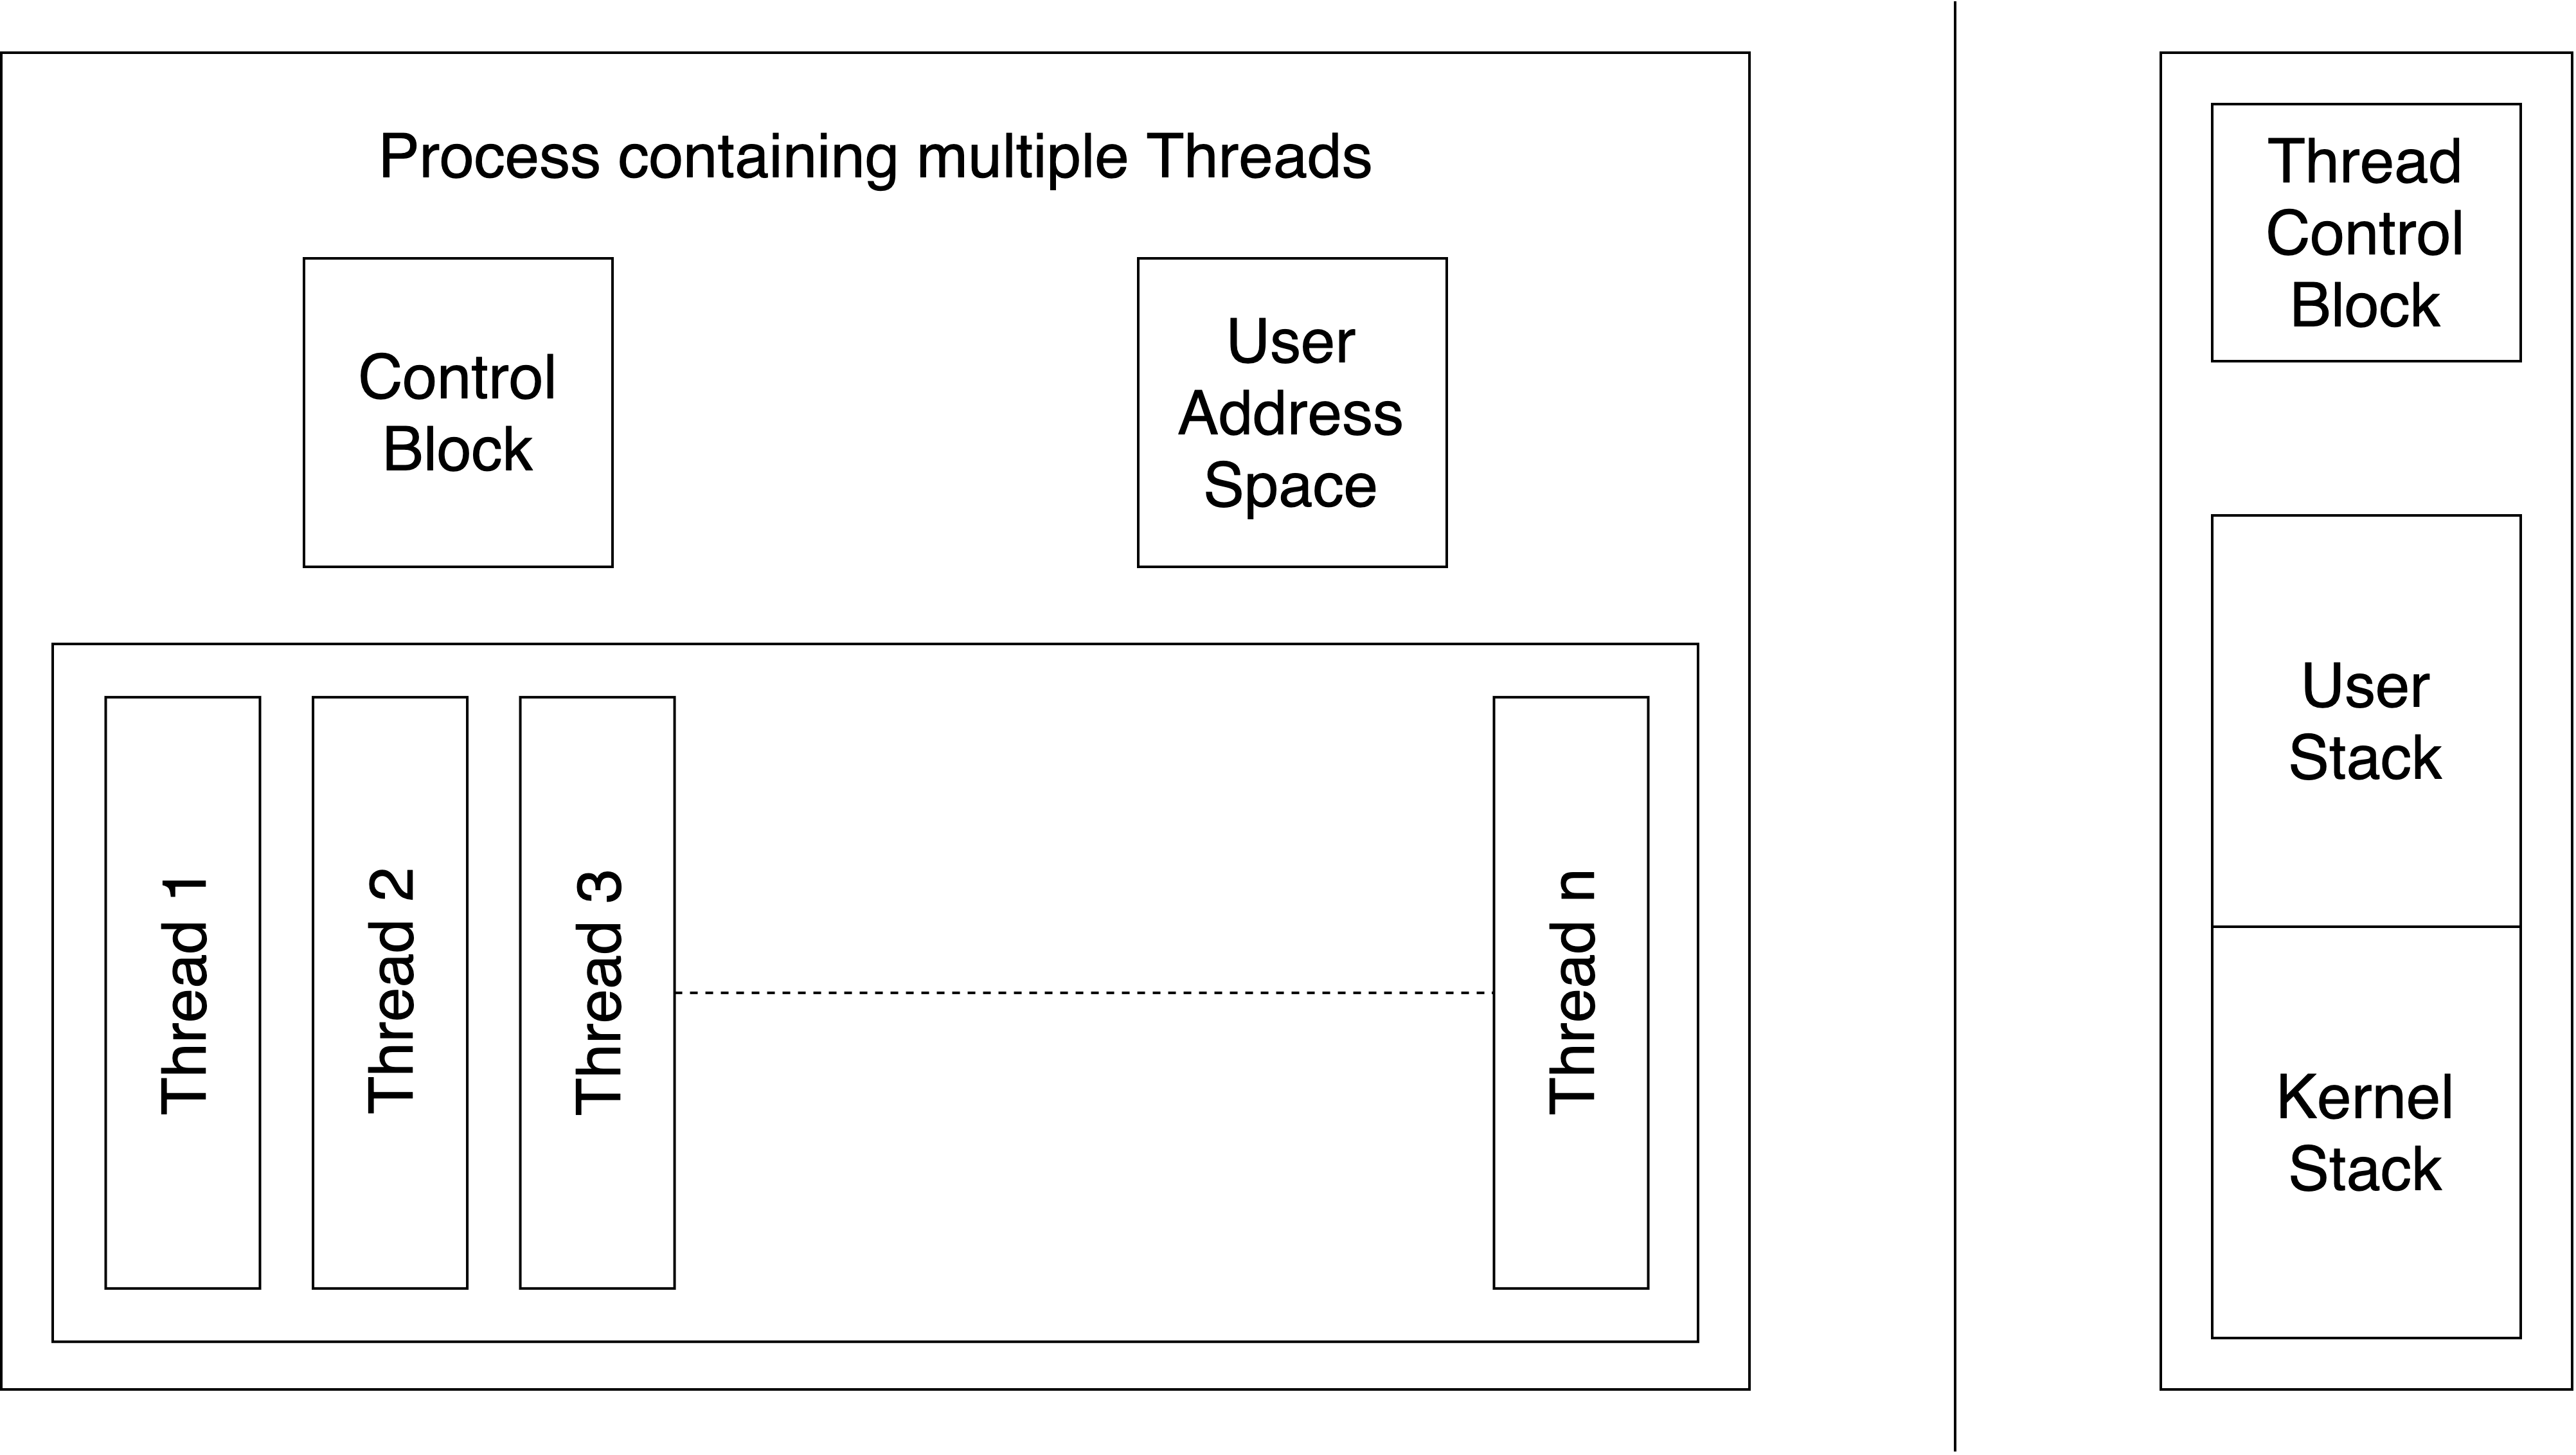
\includegraphics[width=\linewidth]{ThreadOverview.png}
	\caption{Left shows a possible process organization containing multiple threads, right shows an overview of a single thread.}
	\label{fig:threadOverview}
\end{figure}
\par 
An Operating System is capable of multithreading when it has the ability to divide a single process into multiple threads that can be executed concurrently.
When threads can have concurrent paths of execution, this means that the OS has a lot of freedom in scheduling them.
When the current executing thread gets block because of an IO call for example, it can be swapped and a different thread whether or not this thread belongs to the same process.
Multiple threads can be in their execution block at the same time.
That is why this technique is called multi threading, by using this technique the time where the CPU stands idle is vastly reduced.
There are certain dangers with this way of executing. 
One has to be sure that the threads can be swapped places while executing, in other words the result has to be independent from execution order.
This is of course not always the case, the programmer and operating system use tools as "critical sections" to ensure the order where this is necessary.
\par 
Multi core multithreading is the next step. \footnote{The core refers to an available processor each capable of handling their own Instruction Stream. In modern CPU architectures multiple cores are combined on a single CPU.}
This is multi threading where the threads can be divided over the different available processors. 
Here by the speed-up time can be further increased.
However as described earlier concurrency issues can occur especially when every processor has his own cache levels. 
Updated memory locations have to be persistence if necessary throughout the cache levels of all the processors if the data is used in multiple threads. 
This of course limits the actual speed up and when these characteristics are not taken into mind when coding can lead to slower execution times on multi core multi threaded applications compared to single core multithreaded.
However when code is smart designed and the different threads are widely independent and or do not make use of the same memory locations a lot. 
Muli core multithreading can have large advantaged and cause significant speed-up values\footnote{Using Amdahls law to calculate the speed up, as described earlier.}
\subsubsection{High Performance Computing}
High Performance Computing or HPC stands for scaled up version of already fast computer organizations.
There are often referred to as super computers.
HPC systems exist in different architectures and organizations, however in the scope of this thesis two of them are interesting.
\paragraph{GPU}
The super scale version of the GPU.
Multiple powerful GPUs are combined and addressable.

\paragraph{Multi core}
The super scaler version of a multicore pc.
The system is upscalled with hundreds or thousands of available cores, often referred to as nodes.
Those nodes can dynamically be assigned in variating amounts to different projects.

\subsubsection{Cloud Computing}
High performance computing has always been closely connected to universities, study centers or very large companies who have the financial resources to obtain and maintain these systems.
Only in the last decade HPC systems are becoming more available in a service kind of way.
With the introduction of cloud computing companies as amazon, one does not have to own a HPC to use this kind of power.
Cloud services as \textit{Amazon aws} and \textit{Microsoft Azure} offer high performance computing as a service.
This combines the performance benefit of those with a price only relevant to the use.\cite{AmazonWe74:online}\cite{CloudCom84:online}
\subsubsection{Conclusion}
\subsection{OpenMP}
CUDA provides a framework and language extension to execute code on an Nvidia GPU.
Executing a program in parallel on a CPU is a little different.
Modern CPUs and Operating Systems are capable of multithreading.

Controlling threads and their behavior is embedded in all major languages (Java \cite{Defining44:online}, C \cite{Threadsu13:online}, C++ \cite{Threadsu16:online}, C\# \cite{ThreadCl82:online}, Python \cite{threadin24:online}, Swift \cite{ThreadFo70:online}, Kotlin \cite{threadKo75:online}, Fortran \cite{Threadin70:online},...).
However controlling threads is not easy and asks extra skills as well as work hours from programmers.
Because of this, writing parallel code is not always straight forward.
Open MP provides a solution in the form of tags and pragma's.
Instead of focusing on true parallel programming, it let you keep the sequential code and extend it with the correct tags to make it run in parallel.
The tags and pragma's (called directives) are translated by the compiler in correct parallel behavior.
Giving the programmer the freedom to execute code in parallel without introducing the complexity of manual thread management.
\par 
Open MP requires the support of the compiler.
The supported compilers and languages are shown in table~\ref{tab:openMPcompilers}

\begin{table}[]
	\centering
	\begin{tabular}{lll}
		Compiler                      & Language      & Platform                                                                                                                                     \\ \hline
		Absoft Pro Fortran            & Fortran       & Linux, Wondows, Mac OSX                                                                                                                      \\
		AMD                           & C/C++         & Clang based                                                                                                                                  \\
		ARM                           & C/C++/Fortran & Linux                                                                                                                                        \\
		Mercurium                     & C/C++/Fortran &                                                                                                                                              \\
		CCE                           & C/C++/Fortran & Clang Based                                                                                                                                  \\
		Flang                         & Fortran       & Linux                                                                                                                                        \\
		GCC                           & C/C++/Fortran & \begin{tabular}[c]{@{}l@{}}Linux, Solaris, AIX, \\ Mac OSX, Windows,  FreeBSD,\\ NetBSD, OpenBSD, DragonFly BSD,\\  HPUX, RTEMS\end{tabular} \\
		XL                            & C/C++/Fortran & Linux                                                                                                                                        \\
		Intel                         & C/C++/Fortran & Windows, Linux, Mac OSX                                                                                                                      \\
		Lahey/Fujitsu                 & C/C++/Fortran & Fujitsu super computer                                                                                                                       \\
		Clang                         & C/C++         & \begin{tabular}[c]{@{}l@{}}Windows, Solaris, Linux, \\ FreeBSD, Mac OSX\end{tabular}                                                         \\
		Nagfor                        & Fortran       & Windows, Linux, Mac OSX                                                                                                                      \\
		OpenUH Research Compiler      & C/C++/Fortran & Linux                                                                                                                                        \\
		Oracle                        & C/C++/Fortran & Oracle Solaris, Linux                                                                                                                        \\
		PGI                           & C/C++/Fortran & Linux                                                                                                                                        \\
		Texas Instruments             & C             & Custom                                                                                                                                       \\
		Pyjama research compiler Java & Java          & JVM                                                                                                                                         
	\end{tabular}
	\caption{A list of compilers that support OpenMP with their supported platforms.}
	\label{tab:openMPcompilers}
\end{table}
\subsection{Conclusion}
Executing in parallel often seems like a magic phrase.
Something that can easily be done and speedup all your code.
A case can definitely be made pro parallel execution, however it is more complicated than that.
Which can of parallel execution do we prefer and which framework can we use to implement it.
It is very important to distinguish the two largest categories of parallel execution: GPU parallel and CPU parallel.
\section{Matlab with Parallelism}
\subsection{Introduction}
Matlab provides the option to developers to execute code in parallel.
The so called \textit{Parallel toolbox} offers multiple options to achieve parallellism. \cite{Parallel63:online}
\subsection{GPU and CPU parallellism}
As described in the section Parallel Computing, different options of parallel computing exist.
On one side parallellization based on MIMD principles, on the other side based on SIMD principles.
The details can be found in the previous sections.
The \textit{Parallel Computing Toolbox} provides logic related to parallelism based on both MIMD and SIMD systems.
The toolbox uses the ability of the host computer calculate multiple instruction streams on the available cores.
In other words the calculations will be done on the CPU, optimization and memory usage is hidden for the developer and taken care of by the framework itself.
The \textit{Parallel Toolbox} calls every execution stream a worker, and together they are part of a workpool.
In a certain way this closely resembles the behavior of multithreading as described earlier.
\par 
The second parallel computing solution in matlab is the use of the GPU.\cite{MATLABGP8:online}
Functions and tools are provided to make use of an available GPU at time of the execution.
Again, as described earlier the cases where GPU parallellization gives a benefit are specific. 
The biggest example is matrix operations en calculations.
The GPU section of parallelism in the \textit{Parallel Computing Toolbox} makes use of cuda translations.
Therefore it is only available on systems with GPU's that are CUDA enabled.
In real life this is a big restriction because it limits the use to systems with NVidia hardware.

\subsection{Memory management}
When using GPU dedicated computations, the dedicated GPU memory is used. 
It is important te remember that this memory is often smaller than the available CPU memory.
When computations are needed on the GPU, the variables are copied tot the GPU dedicated memory, the computations are done and, if necessary the result is copied back.
The copying of data is the bottleneck in most computer systems, it can be a good idea to leave variables in teh GPU dedicated memory until there is no use for them any more.
The management of these variables in the GPU memory needs to be done by the programmer, hence introducing more complexity into the algorithm.
In most cases the size of matrices is dependent on input of the algorithm and cannot always be foreseen.
A smart memory management system that leaves data longer in the GPU dedicated memory if the data is small and space is available, and copies or divides matrix operations when there is not enough space, is almost a must for robust algorithms.
This introduces a new form of complexity to the algorithm.

\subsection{HPC}
As big as performance benefits can be when introducing parallel execution to your code, it is still limited to your host system and hardware.
Matlab provides the tools for remote execution.
This meaning that a connection can be made with a much more powerful server system in order to gain the benefits of an HPC system while still using the same code as on your machine.
By doing this it limits the develop time to make code projects ready for remote execution enlarging the scalability of projects.
Both server systems with high CPU capacity as GPU servers are supported. \cite{MATLABNV63:online}\cite{MATLABin13:online}

\subsection{Conclusion}
Matlab provides tools to developers to execute code in parallel both on their own device as with an extension to remote execution on servers.
This gives developers/companies a variety of options to execute their code in parallel on both local host devices and cloud service HPCs.


\section{Conclusion}
This concludes the literature review. 
Al the elements from machine learning basic concepts up to fast $v$ fold crossvalidation and HPC computing are introduced and explained.
Meaning that all the base building blocks are now present to start the next objective: analysis of the algorithm in search for suitable parallel execution candidates.



%%%%%%%%%%%%%%%%%%%%%%%%%%%%%%%%%%%%%%%%%%%%%%%%%%%%%%%%%%%%%%%%%%% 
%                                                                 %
%                            CHAPTER                              %
%                                                                 %
%%%%%%%%%%%%%%%%%%%%%%%%%%%%%%%%%%%%%%%%%%%%%%%%%%%%%%%%%%%%%%%%%%% 
\chapter{Research and Investigation}
\section{Introduction}
This chapter serves as an explanation on certain choices that are made.
A chapter like this is in my opinion justified because of a few reasons.
Doing research is not just answering a question, there is a complete process in which a lot of choices have to be made,
and in certain moments, choices need to be revisit. 
Often more than one wrong choice is made but making that wrong choice still contributes to the final result.
In the next sections I will describe my process throughout the past year.
\section{Timeline}
\subsection{Initial Research}
My starting knowledge in the field of machine learning was close to zero.
Therefore the initial research phases consisted mainly of studying the basics of machine learning and different kinds of implementations.
With the basic knowledge built up, I started with the LS-SVM algorithm itself and playing around with the toolbox.
\subsection{Parallel Execution Research}
I started with the idea of running Matlab server on a remote machine and try to make it work.
In my mind this was very useful because the end goal for me at that point was executing parallel code on a remote machine.
However in this process, I had a lot of difficulties with getting the Matlab server to run and to execute code.
\par 
Because it was harder than expected, I started exploring other options.
I knew that a lot of heavy computations were matrix computations.
Matlab is very optimized in matrix computations but not so much in memory management.
The algorithm requires a lot of passing around matrices from one function to another.
If there is one computer language that is perfect for controlling memory and making sure nothing is copied when you don't want to, it is C++.
As a benefit frameworks like OpenMP exist for CPU parallel execution and intelMKL and others for optimized matrix operations on the CPU.
By combining these facts I made the decision to translate the needed functions from Matlab to C++, and to start the development of a C++ FS LS-SVM library.
\subsection{Development}
In the first phase I started with using the Matlab coder toolbox to translate the existing Matlab scripts in the LS-SVM toolbox to c-code.
I quickly found out that:
\begin{enumerate}
	\item Most scripts needed a lot of alterations because the optimized fixed size least square support vector algorithm was not or barely not implemented in the toolbox.
	\item In order to make use of the OpenMp toolbox everything had to be rewritten.
\end{enumerate} 
Manual translation seemed a better option.
I completely separated all the linear algebra from the algorithm in two different libraries.
With the logic that my personal linear algebraic library would be a bridge between an existing optimised framework like intelMKL and the LS-SVM library.
I followed an introduction course to OpenMP at the ICTS center of the KULeuven to get a good start.
OpenMP is, in my opinion, a very good framework that easily gives you a lot of control over parallel threads and making scalability very easy without a lot of environment specifics.
The LS SVM C++ library was quiet easy to develop but the integration with linear algebraic libraries was much more difficult than expected.
Big problems arose with compatibility of the compiler, the use of OpenMp together with the other frameworks and more.
\par 
The compiler settings, paths and cmake files were becoming so environment specific that porting the software from my local machine to a remote machine were becoming impossible.
That together with the fact that without a working optimized linear algebraic framework, it would not be competitive to Matlab execution.
Even with better memory management.
\par 
Those problems forced me to drop all the C++ code and return to Matlab.
The remaining problem: remote execution of the code.
Fortunately, Matlab offers remote execution together with commercial partners in a way that is independent from any environment variables. 
I started adjusting all the needed scripts to optimized FS LS-SVM and creating working models.
\section{Personal Note}
I am aware that this is an odd chapter in a thesis. 
However, for me it is an important one. 
I worked for almost nine months on the C++ library before throwing it all away, meaning that my actual development process was mostly done there and not in the used Matlab code.
This is ofcourse not a waste, I learned C++ programming in a professional way and I am comfortable to say that my knowledge of the OpenMP framework, as well as linear algebraic frameworks as intelMKL, is more than decent.
The biggest downside is that I have investigated less than I hoped to. 
As you will see, there are some very interesting future extensions described in chapter 7 that I actually was hoping to investigate myself.
If there is any interest in my C++ code, I am always willing to open the repositories.



%%%%%%%%%%%%%%%%%%%%%%%%%%%%%%%%%%%%%%%%%%%%%%%%%%%%%%%%%%%%%%%%%%% 
%                                                                 %
%                            CHAPTER                              %
%                                                                 %
%%%%%%%%%%%%%%%%%%%%%%%%%%%%%%%%%%%%%%%%%%%%%%%%%%%%%%%%%%%%%%%%%%% 

\chapter{FS LS-SVM: Analysis of the Algorithm}
\section{Introduction}
In this chapter we look at the FS LS-SVM algorithm in detail.
Every block, every step along the way will get analyzed and the determination will be made if and how a parallelization is possible.
The total performance of the algorithm is discussed to decide which parts are more important.
Meaning which parts of the algorithm would benefit the most with the execution in parallel.
As described in the literature review, executing code in parallel can be divided into two mayor categories.
To simplify we name them:
\begin{itemize}
	\item GPUparallel: code/element would benefit the most of a GPU parallelization.
	\item CPUparallel: code/element eligible for CPU parallelization.
\end{itemize}
The section Linear Algebra describes how matlab can execute matrix computations in parallel, using GPUparallel or CPUparallel.
We start with an analysis of the impact of every element in the total execution time.
\section{Performance measures}
In this section a base algorithm is executed and analyzed in order to determine which elements of the algorithm takes up the most execution time.
Matlab provides a special running mode designed to do just this.
The following data set is used for the testing:
\begin{itemize}
	\item Title: Concrete Compressive Strength\cite{UCIMachi66:online}
	\item Number of attributes: 8
	\item Number of records: 1030
\end{itemize}
The number of support vectors is varied to get a better image of its influence.
The processor on my host machine is a 2,7 GHz Quad-Core Intel Core i7 with 16GB of memory available.
Under the hood Matlab actually makes use of the intelMKL library in order to already optimize the matrix computation over the available cores.
Meaning that a certain level of parallel execution is already present at this base test.
Before running the algorithm, certain values have to be chosen.
\begin{itemize}
	\item Kernel type: RBF kernel
	\item Number of support vectors: 300
	\item Number of folds: 10
	\item SV selection stop after $N/10$ unsuccessful operations.
	\item Starting $\sigma$= 0.75
\end{itemize}
Figure~\ref{fig:prato300} shows a graphical representation of the Pareto plot.
In reality both the tuning phase and support vector selection phase take about the same time. 
With a little side note that this is very dependent on the SV Selection stop criterium.
A faster stop will not only result in a faster SV selection phase but also increase the chance for a non optimal SV set, meaning that the tuning phase might take longer.
Table~\ref{tab:perf} shows the result of the same experiment with 50, 100, 300, 500 and 700 support vectors.
\begin{figure}
	\centering
	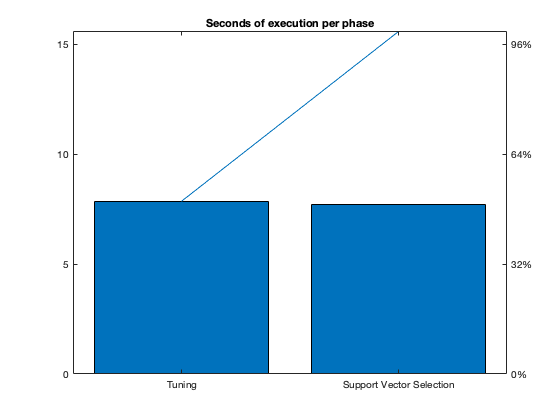
\includegraphics[width=0.8\linewidth]{pareto300.png}
	\caption{The pareto graph when 300 support vectors are used. }
	\label{fig:prato300}
\end{figure}
\begin{table}[]
	\centering
	\begin{tabular}{lll}
		Number of SV             & Selection phase {[}\%{]} & Tuning phase {[}\%{]} \\ \hline
		\multicolumn{1}{l|}{50}  & 54.1                     & 30                    \\
		\multicolumn{1}{l|}{100} & 36.6                     & 48.5                  \\
		\multicolumn{1}{l|}{300} & 48.6                     & 48.1                  \\
		\multicolumn{1}{l|}{500} & 34.1                     & 63.9                  \\
		\multicolumn{1}{l|}{700} & 16.5                     & 81.9                 
	\end{tabular}
	\caption{Values of the performance testing with variable number of SV}
	\label{tab:perf}
\end{table}
Up until 300 support vectors, the tuning phase has results in the same league as the selection phase.
The fact that Matlab uses all four CPU cores gives an advantage here, it makes the tuning phases quiet competitive.
However the performance of the selection is also determent by the fact that the lower the amount of support vector, the higher the chance for finding a better set before the stop criterium is reached, the more iteration are done.
That all being said, as you will see in the following subsection, the tuning phase has more candidates for parallel execution.
\section{Interesting Elements}
This section describes all the different elements of the FS LS-SVM algorithm.
Most of those elements are introduced in the literature review. 
Figure~\ref{fig:fslssvmDetailedOverview} gives a good overview with more details than the overview provided in figure~\ref{fig:fslssvmoverview}.
\begin{figure}
	\centering
	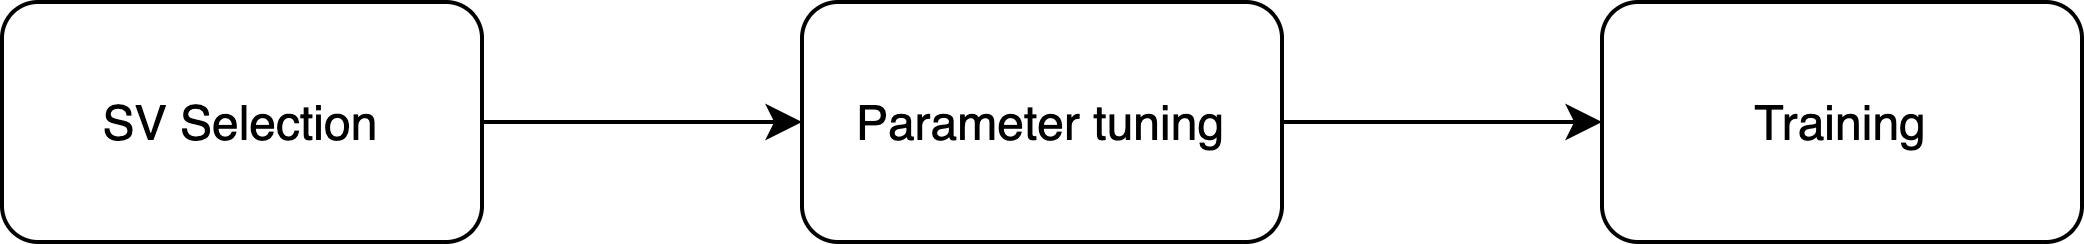
\includegraphics[width=0.8\linewidth]{fslssvm.png}
	\caption{Overview of the different phases of FS LS-SVM.}
	\label{fig:fslssvmoverview}
\end{figure}
Working from outside in, we first can distinguish three phases:
\begin{itemize}
	\item Selection: the search for the best set of support vectors.
	\item Tuning: the search for the optimal model parameters.
	\item Training: the actual model training with the correct set of support vectors and optimal parameters.
\end{itemize}
Outside the three main phases an initial block exists where the starting values and parameters are set and the use block where new data can use the generated model.
In the following subsection the different blocks of the three main phases are discussed.
\subsection{SV Selection}
As described in the literature review, the Support Vector Selection phase is in fact an iteration of the same algorithm with an acceptance phase.
The basic implementation can be found in algorithm~\ref{alg:svselection}.
\begin{algorithm}
	\fbox{\begin{minipage}{\linewidth}
			\SetKwInOut{Input}{input}\SetKwInOut{Output}{output}
			\Input{Model $model$,\\ critStart $cs$}
			\Output{Model $model$ }
			
			// initialization \\
			$Nc$ = $model.Nc$\; Nc represents the amount of support vectors wanted.
			$Xs$ = $model.X$($1$:$Nc$)\;
			$Ys$ = $model.Y$($1$:$Nc$)\;
			$critOld$ = $critStart$\;
			
			\Repeat{Until Stop conditions}{
				// First backup current candidate set \\
				$XsBackup$ =$Xs$\;
				$YsBackup$ =$Ys$\;
				// Generate new candidate set: take previous step and random swap an element \\
				$n$=random(min=1,max=size($model.X$))\;
				$nOld$=random(min=1,max=size($Xs$))\;
				$Xs$($nOld$) = $X$($n$)\;
				$Ys$($nOld$) = $Y$($n$)\;
				
				// Compute new crit value \\
				$crit$ = entropy($Xs$,$model$)\;
				
				// Acceptance condition \\
				\eIf{$crit<critold$}
				{// new candidate set is not accepted\\
					$crit$ = $critOld$\;
					$Xs$ = $XsBackup$\;
					$Ys$ = $YsBackup$\;}
				{// new candidate set is accepted\\
					$critOld$ = $crit$\;
				}	
			}
		// Final Step: assign values of Xs and Ys in model and return model
	\end{minipage}}
	\caption{Basic implementation of the support vector selection algorithm.}
	\label{alg:svselection}
\end{algorithm}
If a small alteration is made, the selection phase is a candidate for parallel execution on the CPU level.
We can state that the loop is going to execute $N$ times.
When the acceptance condition is taken out of the loop, this can be done by storing every set of indices resembling every candidate set and their corresponding criterion value, the loop can be executed in parallel.
An extra step is created because the comparison has to be done after the loop.
With a competitive sorting algorithm, the candidate set can be sorted on the criterion value with a complexity of $nlogn$, $n$ having the same value as number of iterations: $N$.
No computational high demanding matrix operations are performed in this phase, therefor it is not a suitable candidate for GPUparallel execution.
\subsection{Kernels} \label{subsec:kernels}
The function of kernel functions in LS-SVM, and more general in SVM algorithms, is discussed in the literature review.
However in FS LS-SVM the kernel function is computed for the completed data set based only on a selection.
The exact selection that is made by the support vector selection algorithm and handed as an input in this section.
The following assumptions are made:
\begin{itemize}
	\item The complete set of data point consists of $n$ items.
	\item The subset of data points (the selected support vectors) consists of $m$ items.
	\item The specific kernel function that is used in this thesis is called \textit{RBF kernel}, more information and the equation can be found in section~\ref{subsec:kerneltrick}.
	\item The kernel matrix that is constructed will be referred to as $\Omega$.
	\item The features matrix will be referred to as $\Phi$.
\end{itemize}
In the normal LS-SVM approach, the kernel matrix $\Omega$ constructed would be of a dimension $n$x$n$, because of the fact that all $n$ data points are considered support vectors.
With FS LS-SVM, the dimension of $\Omega$ is reduced to $n$x$m$.
This reduces the memory complexity from $\mathcal{O}(n^2)$ to $\mathcal{O}(nm)$, which is significant because $m<<<n$.
\par 
In the FS LS-SVM algorithm the extended feature matrix $\hat{\Phi_e}$ is used.
This matrix represents the bridge in the feature space between the complete data set and the selected support vectors.
To compute this $\hat{\Phi_e}$, a couple of things are required: 
\begin{itemize}
	\item The kernel matrix of the support vectors: $\Omega$.
	\item The kernel matrix between the complete data set and the support vectors $\Omega_N$.
	\item The eigendecomposition of kernel matrix $\Omega$.
\end{itemize}
The Nystr\"om method combines these elements into the features matrix $\hat{\Phi_e}$, as shown in equation~\ref{eq:nystrom}.
\begin{equation}
	\hat{\Phi_e}= repmat(\frac{1}{\sqrt{eigvals(\Omega)}},n).*\Omega_N eigvecs(\Omega)
	\label{eq:nystrom}
\end{equation}
To compute this $\hat{\Phi_e}$, a bunch of matrix operations are needed.
All these operations have their own time and memory complexity that are still strongly dependent on input size $n$, making it a very heavy computational part of the algorithm.
The complexities of each computation is shown in table~\ref{tab:featurescomplexity}.
Figure~\ref{fig:nystrom} shows the feature extraction steps following the Nystr\"om method.
\begin{figure}
	\centering
	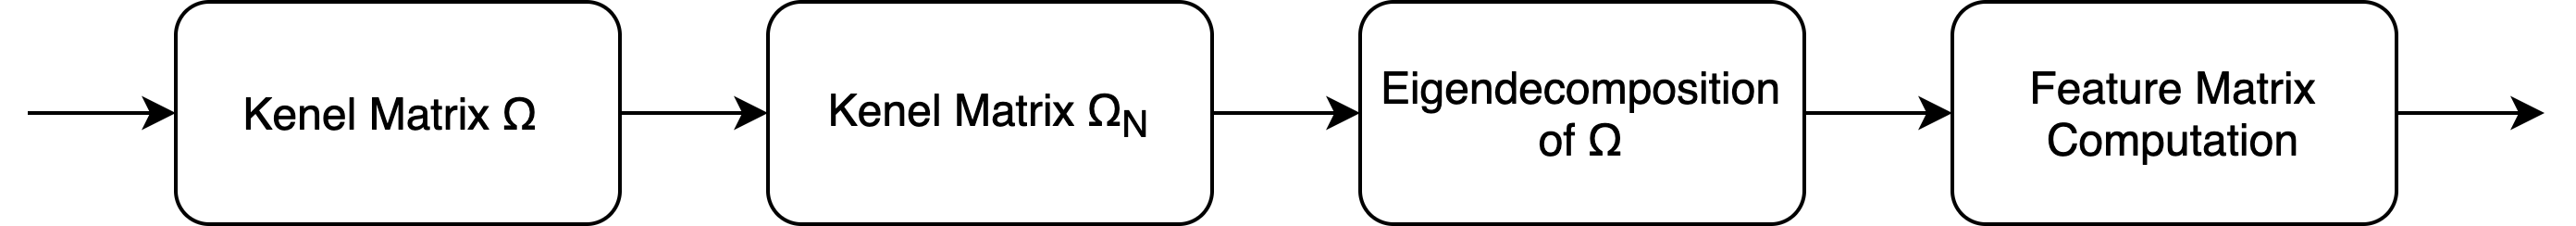
\includegraphics[width=\linewidth]{fastvfoldcrossvalidation.png}
	\caption{Graphical representation of the sequential steps taken in the Nystr\"om method.}
	\label{fig:nystrom}
\end{figure}
\begin{table}[]
	\centering
	\begin{tabular}{lll}
		& Computation Complexity & Memory Complexity  \\ \hline
		\multicolumn{1}{l|}{Kernel Matrix $\Omega$}         & $\mathcal{O}(nm)$      & $\mathcal{O}(nm)$  \\
		\multicolumn{1}{l|}{Kernel Matrix $\Omega_N$}       & $\mathcal{O}(nm)$      & $\mathcal{O}(nm)$  \\
		\multicolumn{1}{l|}{Eigendecomposition of $\Omega$} & $\mathcal{O}(m^3)$     & $\mathcal{O}(m^2)$ \\
		\multicolumn{1}{l|}{Feature Matrix $\hat{\Phi_e}$}  & $\mathcal{O}(nm^2)$    & $\mathcal{O}(nm)$ 
	\end{tabular}
	\caption{Time and memory complexity of the matrix computations used to calculate the feature matrix.}
	\label{tab:featurescomplexity}
\end{table}
Each of those computation is a good candidate for GPUparallel execution.
\subsection{Coupled Simulating Annealing}
CSA is described in detail in the literature review. 
Multiple variants were also introduced, mostly making a difference in the calculation of cost functions.
Often this optimization algorithm is described as $n$\footnote{In this section $n$ does not stand for the number of input data points but it represents the number of coupled values in CSA.} parallel channels of the base SA algorithm coupled together in the cost function.
In my opinion this description can give a good context but is not entirely correct.
In reality it can better be described as a single SA algorithm but instead of taking only one candidate value at a time, it takes $n$.
This does make a big difference for me.
The first formulation suggest that multiple parallel paths can be created that in certain moments have to communicate which each other.
What strongly leans to CPUparallel execution with shared memory.
This is in fact not the case, a single thread has to execute the learning loop, only the calculation of cost values at each evaluation is a candidate for parallel execution.
To make this more clear figure~\ref{fig:parallelcsa} shows a visual representation of the two concepts.
\begin{figure}
	\centering
	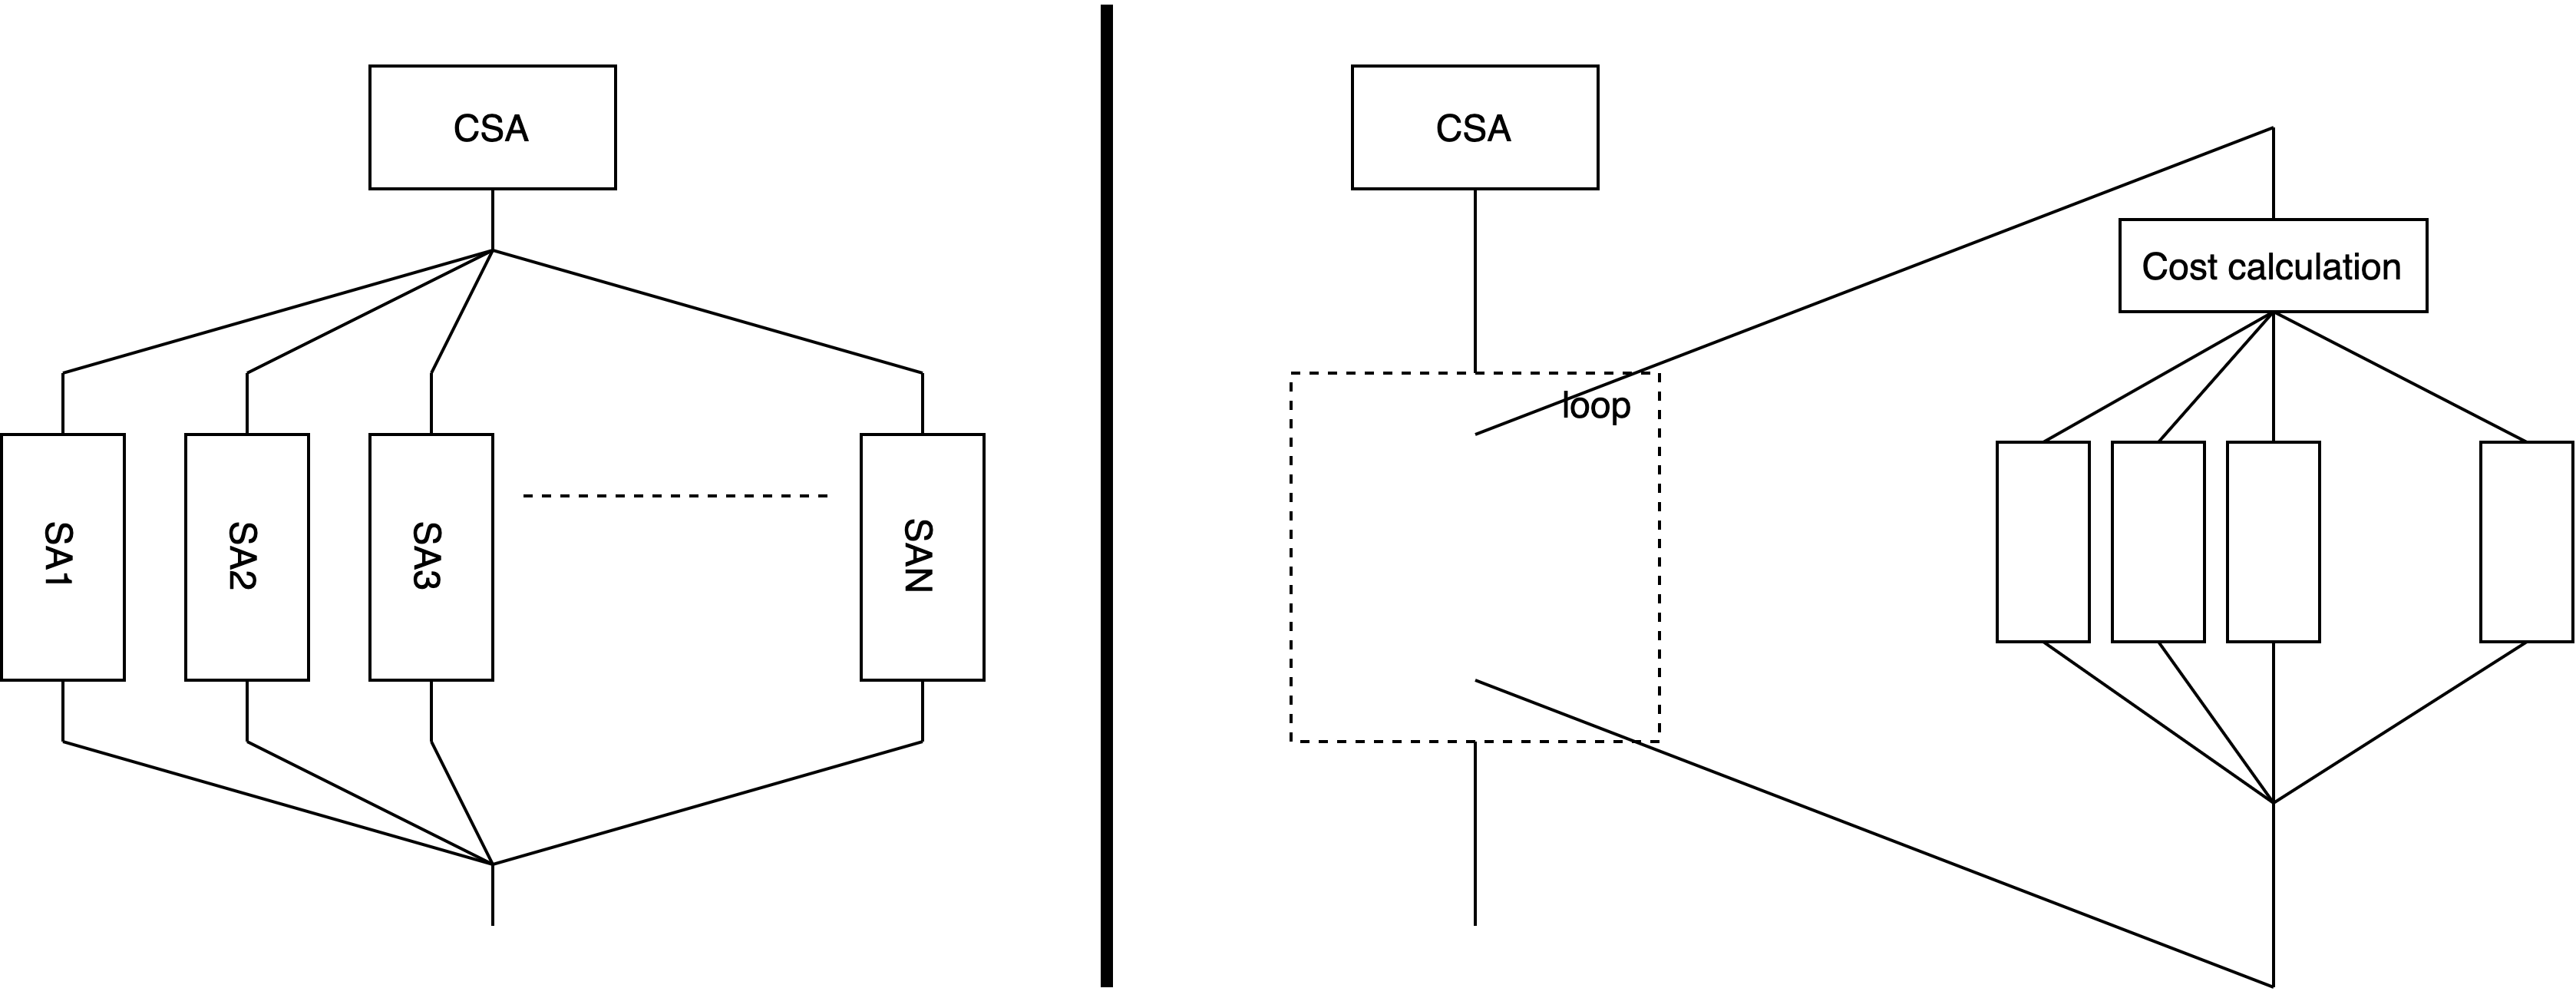
\includegraphics[width=\linewidth]{parallelcsa.png}
	\caption{Left a visualization of csa that is not correct; Right a visualization of parallel csa that comes closer to reality.}
	\label{fig:parallelcsa}
\end{figure}
\par 
If these concepts are clear, we can understand that the CSA algorithm itself does not have parallel execution potential.
However the cost calculation function does have that potential.
In FS LS-SVM and with extension the optimized version \cite{Optimized2010:article}, the cost of a possible solution found by CSA is calculated by the \textit{fast v-fold crossvalidation} algorithm.
Any parallel execution potential of CSA is depended on this function. 
\subsection{Simplex}
The simplex algorithm is used in FS LS-SVM to narrow down the suggestion CSA made for parameter values.
With the objective to find the true optimal values.
When we look at parallelization potential, we see a similar story as with CSA.
The core of the search heuristic consists of a loop that is depended on the result of the previous iteration.
Making it unsuitable for CPUparallel as wel as GPUparallel execution.
However the simplex function also makes use of a cost function and in this case the same function as CSA uses: \textit{fast v-fold crossvalidation}.
This results in the fact that both CSA and simplex export the interesting elements for parallel execution to the same cost function.
\subsection{Crossvalidation}
As described earlier both CSA and simplex heavily rely on a crossvalidation function to calculate the cost of a possible solution.
In the optimized FS LS-SVM the specific crossvalidation function is called \textit{fast v-fold crossvalidation}.
\textit{Fast v-fold crossvalidation} is earlier described in the literature review, this section focuses on the mathematical computations done as well as possible parallel streams.
\paragraph{J Couples}
When we start with a look from the outside, a first thing we notice is that both the CSA and simplex search heuristic send (multiple) couples of values to the crossvalidation algorithm to get a representative performance score.
Meaning that a matrix with dimension $j$x$2$ is sent with input values, the crossvalidation has to run $j$ times, compute an individual score for each entry and at the end combine those scores in to one final representative score for the input set.
This is a perfect case for CPUparallel execution: $j$ different parallel execution paths, independent from each other. 
Of course before exiting the crossvalidation function, the parallel region has to end and a single thread has to execute the combination of the $j$ different scores.
\paragraph{V Folds} 
Diving into a single crossvalidation, we can actually see the same thing happening.
The algorithm consists of a loop that will be executed $v$ times, every time with a different training and validation set.
However the computations done in this loop are not dependent on each other and therefore parallel execution is perfectly possible.
In other words this is also a candidate for CPUparallel code execution.
One iteration of this loop is called a fold, hence the name \textit{fast v-fold crossvalidation}.
\par 
Before the $v$ parallel folds can be started, the feature matrix $\hat{\Phi_e}$, $A$ and $C$ need to be calculated.
This is because every fold takes the complete feature matrix as an input argument, together with the from $\hat{\Phi_e}$ derived matrices $A$ and $C$.
As described in section~\ref{subsec:kernels}, and shown in figure~\ref{fig:nystrom}, this feature extraction consists of a certain amount of sequential steps.
Each step consisting of demanding matrix operations, the complexity is listed in table~\ref{tab:featurescomplexity}.
Every step of this Nystr\"om method is a candidate for GPUparallel code execution.
As shown in figure~\ref{fig:prefold}, after the Nystr\"om method is done, two more computations need to be done before the $v$ folds can start.
These computations, matrix A and C computation, are both candidates for parallel execution and can be calculated at the same time if multiple GPUs are available (or enough GPU cores).
The equations used how to calculate the matrices A and C are shown in section~\ref{subsec:fastvfoldcv}.
Time and memory complexity of both computations is shown in table~\ref{tab:prefold}.
\begin{table}[]
	\centering
	\begin{tabular}{lll}
		& Time Complexity     & Memory Complexity  \\ \hline
		\multicolumn{1}{l|}{Matrix A} & $\mathcal{O}(nm^2)$ & $\mathcal{O}(m^2)$ \\
		\multicolumn{1}{l|}{Vector c} & $\mathcal{O}(nm)$   & $\mathcal{O}(m)$  
	\end{tabular}
	\caption{Time and memory complexity of the prefold calculations}
	\label{tab:prefold}
\end{table}
\begin{figure}
	\centering
	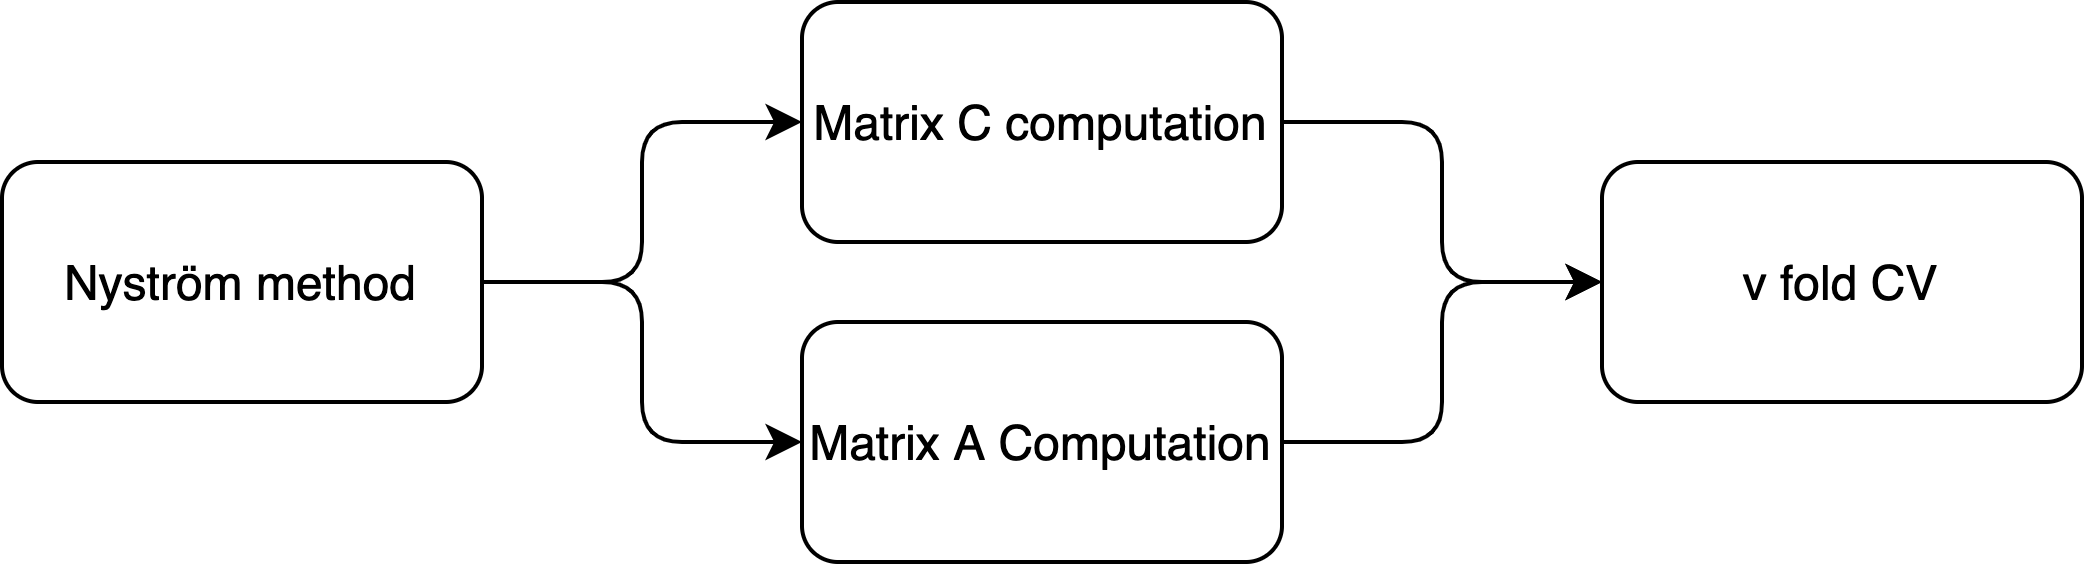
\includegraphics[width=\linewidth]{fastvfoldcrossvalidationAC.png}
	\caption{Graphic representation of the computation steps done before starting the folds.}
	\label{fig:prefold}
\end{figure}
\paragraph{Single Fold}
Every single fold gets the same input arguments: 
\begin{itemize}
	\item Feature matrix $\hat{\Phi_e}$
	\item Trainig data set
	\item fold number $v$
	\item Complete matrix A
	\item Complete vector c
\end{itemize}
Figure~\ref{fig:singleFold} shows the steps taken in a single fold.
Matrix $A_v$ computation, Vector $c_v$ computation and the Linear Equation Solving are suitable candidates for GPUparalle execution.
They are in fact just matrix operations.
Equation~\ref{eq:linearsystemfold} shows the linear Equation Solving, taking as an input both $Av$ and $Cv$.
Equation~\ref{eq:Avfold} shows how to compute $A_v$.
Equation~\ref{eq:cvfold} shows how to compute $c_v$.

\begin{figure}
	\centering
	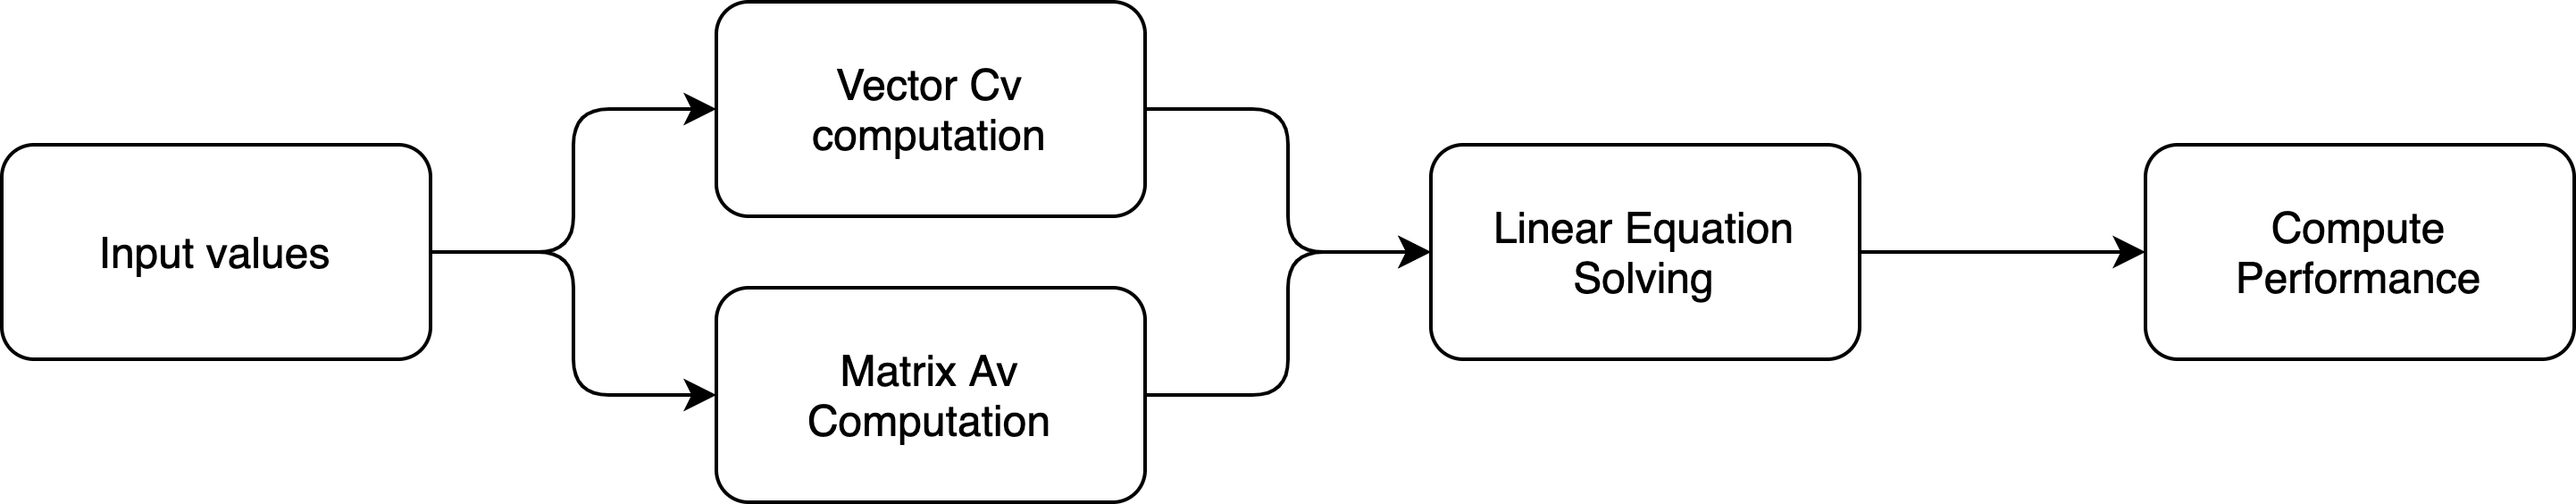
\includegraphics[width=\linewidth]{fastvfoldcrossvalidationSingleFold.png}
	\caption{Graphical representation of the steps in a single fold.}
	\label{fig:singleFold}
\end{figure}
\begin{equation}
	\binom{\hat{w}}{\hat{b}} = A_v^{-1}c_v
	\label{eq:linearsystemfold}
\end{equation}
\begin{equation}
	A_v = A - \left(\frac{\hat{\Phi}_{val}^T}{1_{val}^T}\right)  \left(\hat{\Phi}_{val} 1_{val}\right)
	\label{eq:Avfold}
\end{equation}
\begin{equation}
	c_v = c - \left(\frac{\hat{\Phi}_{val}^T}{1_{val}^T}\right)Y_{val}
	\label{eq:cvfold}
\end{equation}
For the first time a parallel execution difficulty occurs.
When executing both $J$ couples and $v$ folds in CPU parallel, a nested parallel execution is created.
This is a difficulty because a distribution has to be chosen, the available parallel streams have to be divided between the needed paths.
When a equal distribution is chosen and for example four parallel paths can be created, the situation is described in figure~\ref{fig:nestedparallel}.
\par
The second parallel execution difficulty that occurs is the possible simultanious computation of $A$ - $c$ and $A_v$ - $c_v$.
This is theoretically possible but not easy to achieve in Matlab, where in the end there is limited control over what ends up where and is executed how on the GPU.
\begin{figure}
	\centering
	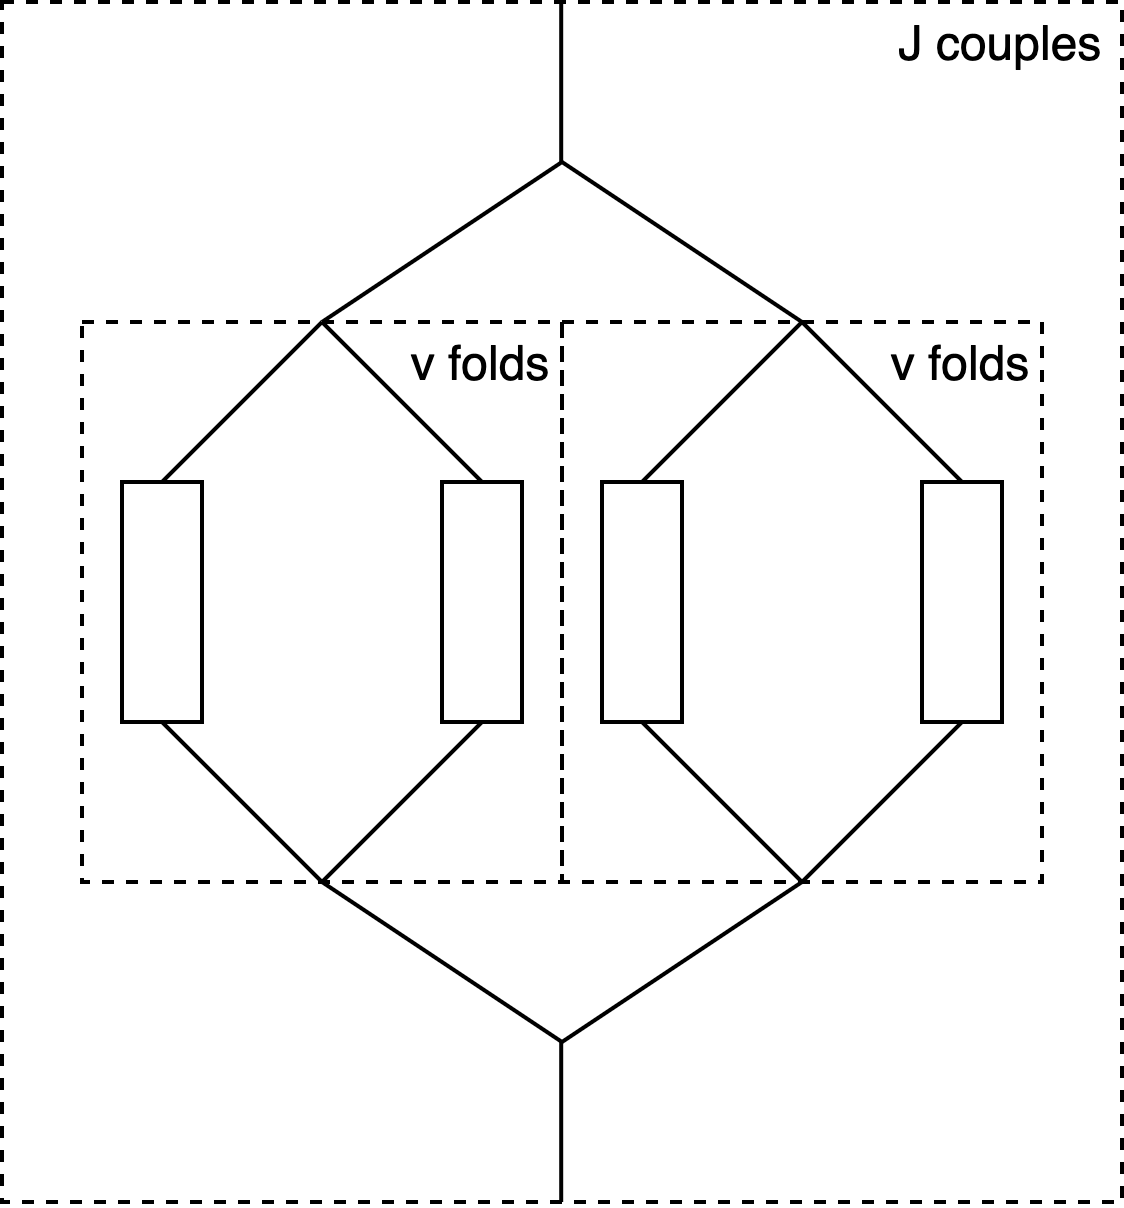
\includegraphics[width=0.8\linewidth]{nestedparallel.png}
	\caption{Graphical representation of the nested parallel region.}
	\label{fig:nestedparallel}
\end{figure}
\section{Conclusion}
Looking at the complete picture, multiple elements qualify for parallel execution.
Both CPUparallel and GPUparallel execution.
Table~\ref{tab:parcandidates} shows a complete lists of all the elements.
An extra layer to add is that this analysis covered the core of the algorithm.
Extra elements might appear when choosing a certain use case, meaning that function estimation, classification and multi-classification each have their specific logic at some points.
Especially when looking at multi-classification, depending on the chosen coding, a certain amount of models have to be created. 
Each of these models can be calculated in parallel of each other as they actually do not depend on data from each other.
Another side note is the competitiveness of models.
In certain cases to enhance the competitiveness of a solution, multiple models are created for the same case and the one with the highest performance score (or lowest error score) is chosen as a final solution.
If that is applied, it can be done perfectly in parallel streams.
When speaking about multi-classification and competitiveness we are in both cases talking about CPUparallel code execution possibilities.
\par 
Returning to table~\ref{tab:parcandidates}, as earlier described there are two different categories: CPUparallel and GPUparallel.
Each candidate is given a status for those two categories.
The possibilities for a status are: possible, possible yet not ideal and not possible.
Those three statuses are possible because every matrix operation can be executed in parallel on a CPU, only this is not ideal.
The performance gain by executing matrix operation in parallel on a GPU is much larger, hence the possible yet not ideal CPUparallel status for every candidate that has a GPUparallel possible status.
\par
Two parallel execution difficulties made their introduction in certain elements: nested parallel and simultaneous GPU execution. 
\begin{table}[]
	\centering
	\begin{tabular}{lll}
		& CPUparallel            & GPUparallel  \\ \hline
		\multicolumn{1}{l|}{SV selection}                        & possible               & not possible \\
		\multicolumn{1}{l|}{$J$ couples}                         & possible               & not possible \\
		\multicolumn{1}{l|}{Kernel Matrix $\Omega$}              & possible yet not ideal & possible     \\
		\multicolumn{1}{l|}{Kernel Matrix $\Omega_N$}            & possible yet not ideal & possible     \\
		\multicolumn{1}{l|}{Eigendecomposition of $\Omega$}      & possible yet not ideal & possible     \\
		\multicolumn{1}{l|}{Features Computation $\hat{\Phi}_e$} & possible yet not ideal & possible     \\
		\multicolumn{1}{l|}{Matrix A}                            & possible yet not ideal & possible     \\
		\multicolumn{1}{l|}{Vector c}                            & possible yet not ideal & possible     \\
		\multicolumn{1}{l|}{$V$ folds}                           & possible               & not possible \\
		\multicolumn{1}{l|}{Matrix $A_v$}                        & possible yet not ideal & possible     \\
		\multicolumn{1}{l|}{Vector $c_v$}                        & possible yet not ideal & possible     \\
		\multicolumn{1}{l|}{Linear System Solving}               & possible yet not ideal & possible    
	\end{tabular}
	\caption{List of elements that can be executed in parallel.}
	\label{tab:parcandidates}
\end{table}
%%%%%%%%%%%%%%%%%%%%%%%%%%%%%%%%%%%%%%%%%%%%%%%%%%%%%%%%%%%%%%%%%%% 
%                                                                 %
%                            CHAPTER                              %
%                                                                 %
%%%%%%%%%%%%%%%%%%%%%%%%%%%%%%%%%%%%%%%%%%%%%%%%%%%%%%%%%%%%%%%%%%% 

\chapter{Parallel Fixed Size Least Square Support Vector Machines in Action }
\section{Introduction}
This chapter describes the actual testing done on the parallel version of Fixed Size Least Square Support Vector Machines.
The different tests are described as well as why they are necessary.
An hypothesis for each test is made with a reasonable explanation.
The test results are presented and a conclusion about the test process ends this chapter.\footnote{This is not a conclusion of the general objectives that were stated.}
\section{What To Test}
For all the testings we use two different data sets.
The first dataset is considered small to medium size, consisting of the following characteristics:
\begin{itemize}
	\item Title: Concrete Compressive Strength\cite{UCIMachi66:online}
	\item Number of attributes: 9
	\item kernel type: RBF kernel
	\item Number of data points: 1030
	\item Type: function estimation
\end{itemize}
With a size of 1030 elements, this data sets allows execution on a personal computer.
This is important to do initial testing and set base characteristics of the behaviour.
\par 
The second data set has the following characteristics:
\begin{itemize}
	\item Title: YearPredictionMSD Data Set\cite{UCIMachi93:online}
	\item Number of attributes: 90
	\item Kernel type: RBF kernel
	\item Number of data points: 515345
	\item Type: function estimation
\end{itemize}
With a size of more than 500 000 data points and more than 50 attributes this can be considered a, so called, big data set.
It is still possible to execute the algorithm with this data set on a personal computer but the performance will decrease drastically.
\par 
To make adequate performance conclusions, multiple tests need to be completed.
A base indicator of computing time is found by executing both data sets on a personal computer in a non parallel matter.
These results will not have any meaning in the final conclusion but give a good indication of the computational time we are dealing with.
\par 
The serious tests will be done on a much more powerfull machine. 
In the original objective a HPC was mentioned as a host machine.
As described in the literature review, the term HPC is very vague and can include multiple types of machines.
I decided to use the service based approach\footnote{This is as well described in the literature review.}.
NVIDIA supports Matlab cloud computing with Amazon Web Services.
This is done using an ubuntu virtual machine on the AWS servers, connected to both a powerful CPU and GPU.
The virtual machine runs a Matlab docker container.\cite{MATLABDe46:online}
This specific setup and docker container is called MATLAB Deep Learning Container on NVIDIA GPU Cloud.
The hardware specifics are shown in figure~\ref{fig:awsspec}.
\begin{figure}[H]
	\centering
	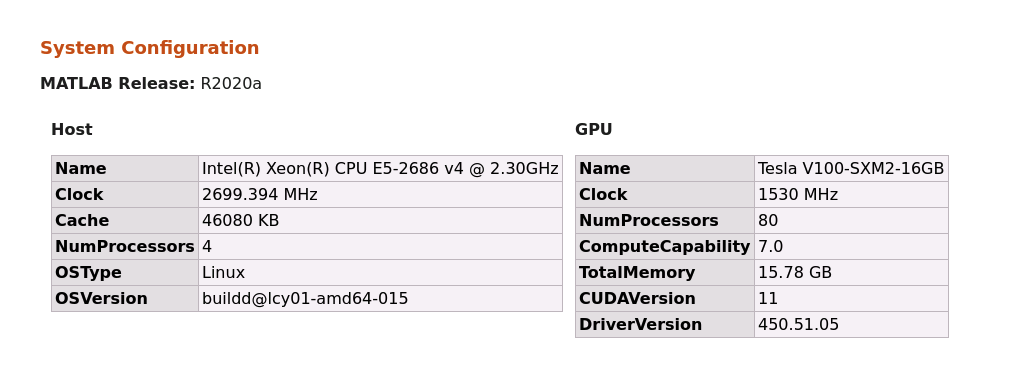
\includegraphics[width=\linewidth]{awsSpecifications.png}
	\caption{The hardware specifications of the test bench used in the MATLAB Deep Learning Container on NVIDIA GPU Cloud.}
	\label{fig:awsspec}
\end{figure}
In the appendices chapter, this setup is discussed with more details.
\par 
On this test bench setup, both data sets need to be tested in both sequential and parallel execution to achieve representative performance results.
\subsection{Sequential}
The sequential execution is needed to set a base mark.
Without a base mark, execution times of parallel code blocks will not have any meaning. 
\subsubsection{On Device Execution}
The on device sequential test with the small dataset has the following characteristics:
\begin{itemize}
	\item Title: Concrete Compressive Strength\cite{UCIMachi66:online}
	\item Number of attributes: 9
	\item Kernel type: RBF kernel
	\item Number of support vectors: [10, 50, 100, 300, 700, 730]
	\item Number of folds: 10
	\item SV selection stop after $N/20$ unsuccessful operations.
	\item Starting $\sigma$= 0.75
	\item Times of execution: 25
\end{itemize}
The on device sequential test with the large dataset has the following characteristics:
\begin{itemize}
	\item Title: YearPredictionMSD Data Set\cite{UCIMachi93:online}
	\item Number of attributes: 90
	\item Kernel type: RBF kernel
	\item Number of support vectors: 730
	\item Number of folds: 10
	\item SV selection stop after $N/10000$ unsuccessful operations.
	\item Starting $\sigma$= 0.75
	\item Times of execution: 1
\end{itemize}
This test is only going to be executed once because the data set is so large and the execution time on my personal device is not going to be representative for performance comparison.
\subsubsection{HPC execution}
The HPC sequential test with the small dataset has the following characteristics:
\begin{itemize}
	\item Title: Concrete Compressive Strength\cite{UCIMachi66:online}
	\item Number of attributes: 9
	\item Kernel type: RBF kernel
	\item Number of support vectors: [10, 50, 100, 300, 700, 730]
	\item Number of folds: 10
	\item SV selection stop after $N/20$ unsuccessful operations.
	\item Starting $\sigma$= 0.75
	\item Times of execution: 25
\end{itemize}
The HPC sequential test with the large dataset has the following characteristics:
\begin{itemize}
	\item Title: YearPredictionMSD Data Set\cite{UCIMachi93:online}
	\item Number of attributes: 90
	\item Kernel type: RBF kernel
	\item Number of support vectors: [700, 1500, 2000, 2500]
	\item Number of folds: 10
	\item SV selection stop after $N/10000$ unsuccessful operations.
	\item Starting $\sigma$= 0.75
	\item Times of execution: 25
\end{itemize}
This test is going to be executed 25 times to achieve good base results for the sequential execution times for multiple numbers of support vectors.
\subsection{Parallel}
The parallel testing is done on slightly altered code. 
All the candidates defined in chapter 4 are coded in the correct manner.
In the appendices is shown how parallel executable code is written in Matlab.
\subsubsection{On Device Execution}
On device parallel test is not possible due to a lack of CUDA support.
In the entirely this does not matter because the real comparison is made between sequential an parallel execution on the HPC.
However this directly point to the restriction of GPU parallel computing as described in the literature review.
\subsubsection{HPC Execution}
The HPC parallel test with the small dataset has the following characteristics:
\begin{itemize}
	\item Title: Concrete Compressive Strength\cite{UCIMachi66:online}
	\item Number of attributes: 9
	\item Kernel type: RBF kernel
	\item Number of support vectors: [10, 50, 100, 300, 700, 730]
	\item Number of folds: 10
	\item SV selection stop after $N/20$ unsuccessful operations.
	\item Starting $\sigma$= 0.75
	\item Times of execution: 25
\end{itemize}
The HPC parallel test with the large dataset has the following characteristics:
\begin{itemize}
	\item Title: YearPredictionMSD Data Set\cite{UCIMachi93:online}
	\item Number of attributes: 90
	\item Kernel type: RBF kernel
	\item Number of support vectors: [700, 1500, 2000, 2500]
	\item Number of folds: 10
	\item SV selection stop after $N/10000$ unsuccessful operations.
	\item Starting $\sigma$= 0.75
	\item Times of execution: 25
\end{itemize}
This test is going to be executed 25 times to achieve good base results for the parallel execution times for multiple numbers of support vectors.
\section{What To Measure}
The decision is made to measure the complete execution time.
This is a good indicator because it provides a total speed-up of the algorithm. 
The following things have to be taken into account:
\begin{itemize}
	\item The dataset will be loaded into Matlab every time. Relevant because this is a sequential task that is always going to be a bottleneck even when every detail of the algorithm is optimized.
	\item The SV Selection is also part of the time measurement. Relevant because: however the fact that it is mostly a sequential task, it does call the kernel matrix function which is parallelized, and it is a major part of the algorithm that contributes to the total performance characteristic of the FS LS-SVM algorithm.
\end{itemize}
\section{Hypothesis}
Knowing that copying data to and from the GPU dedicated memory creates extra overhead and that the Intel Xeon processor is quiet powerful, I suspect that matrix computations and alterations with small dimensions are not going to lead to a performance increase.
Translating this to my test cases: I do not expect an execution time speed up for the small data set comparing parallel and sequential execution on the HPC.
I suspect larger execution times for small number of support vectors and at the same time much better results for large number of support vectors.
Somewhere is going to be a critical point where it becomes beneficial to use the parallel execution.
Because of the fact that Matlab uses optimization on the CPU and that the HPC CPU is quiet powerful, I suspect the critical point to be just higher than the max amount of support vectors in the small data set (higher than 700). 
An exact speed-up prediction number is hard to calculate because that is very dependent on the following items:
\begin{itemize}
	\item GPU frequency (known)
	\item GPU percentage of used GPU cores for computations (hard tot calculate and very data set specific)
	\item Data transfer speed (unknown)
	\item CPU multi core optimization (unknown, hard to quantify) 
	\item CPU frequency (known)
	\item Exact percentage of parallel code (estimation possible but not exact)
	\item Overhead with CPU execution when main memory elements have to be swapped (impossible to predict/calculate)
\end{itemize}
Because of the fact that the \textit{fast $v$ fold crossvalidation} algorithm is called so many times in this algorithm, a large number of data transfers is needed.
The impact of the needed time, and overhead created for cpu to manage this transfer is out of my knowledge to calculate and most important will have a significant impact on the total execution time when executing code in parallel.
This results in the fact that the equation of Amdahls' law\ref{eq:amadahl} cannot provide us with a representative result
Therefore I double down on the hypothesis made earlier that not all test cases are going to result in a speed up because of the hard calculate overhead and hard to quantify already present optimization of the available CPU cores by Matlab.\footnote{In case of Intel processors Matlab is using intel mkl for blas optimization}
\section{Test Results}
\subsection{Problems}
When starting the execution of the different tests, problems occurred in the \textit{fast $v$ fold crossvalidation} function.
As described in chapter 4, this section exists of a nested CPUparallel region with both in and before the second region multiple GPUparallel computations.
The parallel computing toolbox does not provide the same amount of control compared to C++ frameworks for multithreading\footnote{Hence the initial choice for C++ and OpenMP.}.
Matlab struggles interpreting variables, especially in combination with GPU combined usage.
On top of that, with large data sets and large numbers of support vectors, the used amount of memory on the GPU rises quickly, when in that case multiple pool workers (CPU threads) call the GPU for dedicated matrix computations a bottleneck in GPU memory rises.
When making use of 700 or more support vectors, CPU parallel execution of the $J$ couples and $v$ folds of the \textit{fast $v$ fold crossvalidation} algorithm became impossible, even on the NVIDIA Tesla v-100 GPU.
Therefore alterations were made to execute $J$ couples and $v$ folds sequential while maintaining the GPU parallel execution for all other regions as described in table~\ref{tab:parcandidates}.
\subsection{Results After Alteration}
As described in this chapter, every test on the HPC is run at least 25 times for every tested number of support vectors to get a stable result.
The mean of the execution time is calculated for every number of support vector used.
The results for the small data set can be found in table~\vref{tab:resultssmall} and shown in figure~\ref{fig:smallresult}.
\begin{table}[]
	\centering
	\begin{tabular}{l|llllll}
		Number of SV 		& 10          	& 50         & 100         & 300        & 700       & 730    \\ \hline
		On device Sequential [s]   	& 0,732  	   	& 1,090  	 & 2,104 	   & 9,809 	& 52,628 	& 55,696 \\
		HPC Sequential [s]   	& 0,676  	   	& 1,455  	 & 2,465 	   & 10,367 	& 39,686 	& 42,621 \\
		HPCParallel   [s]  	& 4,661  	   	& 5,236  	 & 6,082  	   & 16,257 	& 30,528  	& 29,991 \\ \hline
		HPC Seq/Par      		& 0,144  	   	& 0,278	     & 0,405	   & 0,637 		& 1,300 	& 1,421
	\end{tabular}
	\caption{Small data set results: the mean execution times in seconds for every number of support vectors, Seq/par row shows the corresponding speed-up factor.}
	\label{tab:resultssmall}
\end{table}
The results for the large data set can be found in table~\vref{tab:resultslarge}.
\begin{table}[]
	\centering
	\begin{tabular}{l|lll}
		Number of SV       & 700      & 1500     & 2000 		\\ \hline
		On device Sequential [s] & 2854,697 & / &  /    \\
		HPC Sequential {[}s{]} & 2295,078 & 6863,830 &  9504,194    \\
		HPC Parallel {[}s{]}   & 119,970  & 547,007  &  1064.495	 \\ \hline
		HPC Seq/Par            & 19,130   & 12,548   &  8,928   			
	\end{tabular}
\caption{Large data set results: the mean execution times in seconds for every number of support vectors, Seq/par row shows the corresponding speed-up factor.}
\label{tab:resultslarge}
\end{table}
\begin{figure}
	\centering
	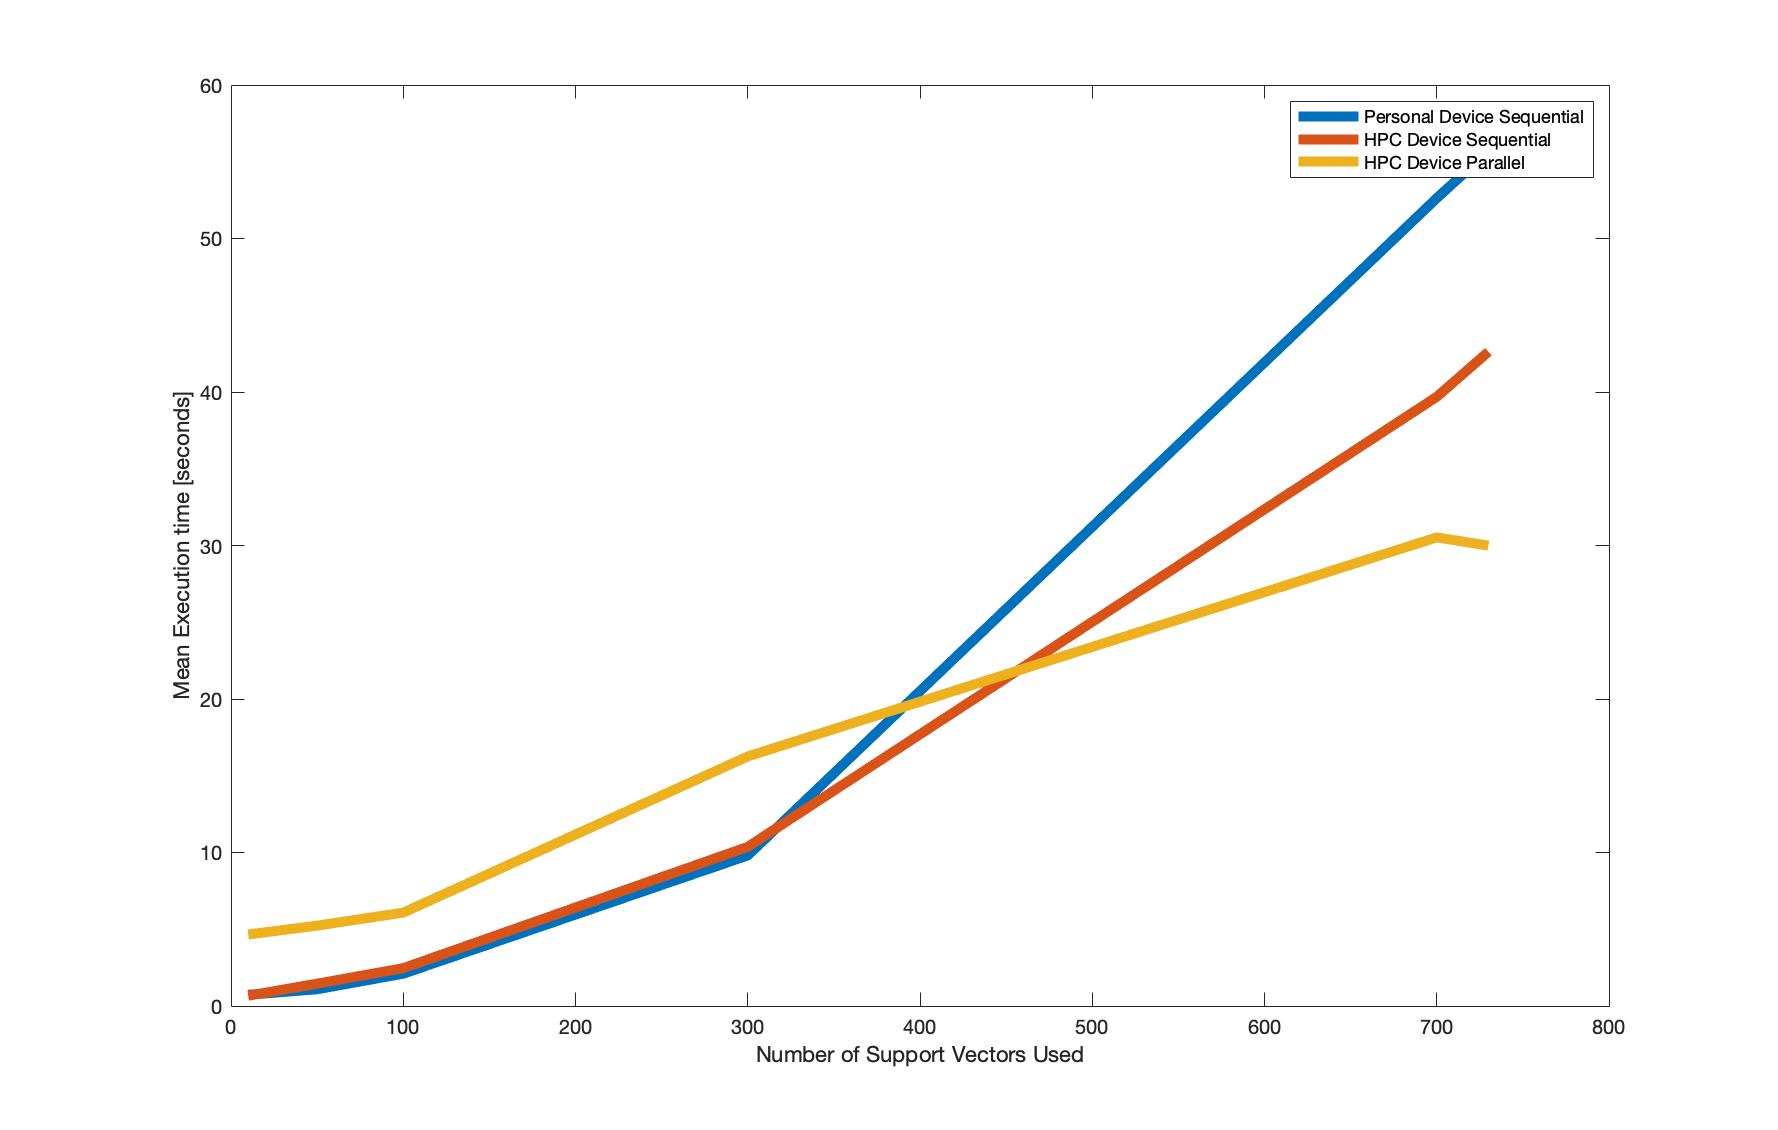
\includegraphics[width=\linewidth]{smallresult.png}
	\caption{Mean values of the execution times on the small data set.}
	\label{fig:smallresult}
\end{figure}
\section{Conclusion}
When looking at the results and taking into account the hypothesis made, a few things stand out.
First, as stated the overhead introduced by copying data back and forth from the main memory to GPU dedicated memory combined with the optimized execution on th CPU does result in worse parallel execution times for a low amount of support vectors.\par 
Looking at the results of the small data set this really stands out for 10, 50 and 100 support vectors.
Resulting in a corresponding speed up factor of way below one. 
What stands out is that the tipping point, where parallel execution becomes interesting is locates at an amount of support vectors below 700.
Because of the power of the CPU this is something I did not expect.\par 
Looking at the results of the large data set, the speed-up factor even for 700 support vectors is way higher compared to the small data set.
The reason behind this has to do with the all the computations done in the FS LS-SVM algorithm.
As described earlier, most operations are with matrices of size $m$\footnote{$m$ stands for the number of support vectors}, but at some points the full data set is still taken into account.\footnote{(Extended) Feature matrix computation and more}.
This results in the fact when dealing with a large dataset the benefit of using GPUparallel execution is going to be larger than with a smaller dataset even when using the same amount of support vectors.






%%%%%%%%%%%%%%%%%%%%%%%%%%%%%%%%%%%%%%%%%%%%%%%%%%%%%%%%%%%%%%%%%%% 
%                                                                 %
%                            CHAPTER                              %
%                                                                 %
%%%%%%%%%%%%%%%%%%%%%%%%%%%%%%%%%%%%%%%%%%%%%%%%%%%%%%%%%%%%%%%%%%% 

\chapter{Conclusion}
When making the literature review it stood out that the amount of matrix operation used in Machine Learning algorithms in general and Support Vector Machines algorithms specific, makes it a very suitable candidates for GPU parallel execution.\par 
Secondly it also stood out that the different ways to accomplish parallel execution provided us with multiple options to work with.
When diving into the LS-SVM algorithm, the Fixed Size LS-SVM algorithm and the later optimized FS LS-SVM algorithm, it became quiet clear that large matrix operations are together with a correct search of the Support Vectors set are the main bottleneck of the algorithm.\par
A detailed analysis of the algorithm provided us with all the elements that are suitable candidates for parallelization in any form.
\par
After seeing more benefits in full control over multiple CPU threads and memory management, I made the initial choice to work in C++.
However the fact that in CPU multi threading the results were very promising and the personally made coding libraries were working fine, the connection between the multi threading and vectorization framework not only proved to be too hard, it also proved to be too environment specific.
Therefore the decision was made to return to Matlab and use the parallel computing toolbox.
The sacrifices of full control in threads and memory were made for the more high level usage of Matlab scripting language with a better chance of accomplishing working models.
\par
With returning to Matlab and constructing my personal Matlab scripts for the FS LS-SVM algorithm, based on the existing LS-SVM toolbox, and literature provided to me about the FS LS-SVM and optimized FS LS-SVM algorithm.
After testing this algorithm provided me with realistic results proving that it worked.
With the completion of a working yet still sequential model, the pre-objectives of my thesis were met.
I was in possession of thoroughly literature review, algorithm analysis and a working sequential model.
\par 
Considering the testing hypothesis I did not predict a speed-up factor because of multiple hard to calculate or quantify factors.
What I did do is predict phenomena based on literature knowledge about the working of GPU usage and Matlab memory management.
As expected a tipping point exist from when the performance of GPU parallel code exceeds the non GPU parallel code.
As also expected, the advantage of large data sets is bigger compared to small data sets, even over the same amount of Support Vectors used.
When looking at the large data set we notice a speed-up factor of more than 10.
A large speed-up factor was expected but with the knowledge I have right now, I would like to make some remarks.
Speed-up factor is the ideal term because it only talks about the difference in execution time.
This is ideal because it only gives us information about the time. 
As described in the hypothesis section of the previous chapter a lot of factors are involved were some are hard to quantify.
The biggest example is memory management: because most of the matrix computations happen inside the crossvalisation, most matrices are not copied back to the main memory.
This gives a significant difference, it results in the fact that all those large matrix files (worst case size $n$x$m$ or vice versa) do not exist in main memory.
When working with large data sets it results in the fact that Matlab is going to need less main memory swaps, reducing the CPU main memory management.
This phenomenon does not have anything to do with parallel execution therefor in my opinion speed-up factor is an ideal term, not too narrow connected to parallel execution alone.
\par 
The tests of the large data set are situated in an ideal spot: the matrices are large enough to take full advantage of the GPU capabilities but at the same time all the matrices used in the crossvalidation can coexist in the dedicated GPU memory.
If the data set and or the number of support vector gets larger, intermediate memory management is needed in the \textit{fast $v$ fold crossvalidation} algorithm introducing extra overhead time.
As described in the literature review, Matlab does not take care of memory management on the GPU, this needs to be implemented in the algorithm itself.
\par 
As shown in the test results, small data sets and or working with a small number of support vectors does not provide a reduce in execution time.
The conclusion can be made that however the HPC GPU provides a big performance benefit, not all cases can fully benefit from it.
When thinking about training models on such a high performance machine the alteration should always be made if it provides a benefit.
\par  
The alterations in the tests needed to be able to get a valid result were not part of my plan.
The fact that CPU thread control is harder in Matlab and that it is not that transparent was one of the original reasons that I chose to implement the algorithm in C++.
When returning to Matlab implementation this was the biggest trade off made.
However I do think this is possible but a complete rewrite of the variable structure in the algorithm is needed and dedicated GPUs for every worker\footnote{worker in Matlab has the same functionality as a thread.} would be ideal.\footnote{I am not aware if it possible to dedicate a single GPU to a single worker in the Matlab scripting language}
\par 
With the development of a parallel FS LS-SVM algorithm, the testing on a HPC device and the use of a data set of more than 500000 data points and more than 50 attributes, most of the objectives are met. 
However the implementation of binary classification has not been, with the switch back from C++ to Matlab I did not have the time to complete the binary classification parallel implementation and testing. 
This is a petty because if I made the switch earlier I am sure I would have some interesting results as well.
With more time I would have rewritten the cross validation in order to make it Matlab CPUparallel proof and/or I would have tried to find different HPC testing setups.
But it is what it is, most of the stated objectives are met and in my opinion with very intersting results.
In the next chapter some possible extensions are listed.

 



%%%%%%%%%%%%%%%%%%%%%%%%%%%%%%%%%%%%%%%%%%%%%%%%%%%%%%%%%%%%%%%%%%% 
%                                                                 %
%                            CHAPTER                              %
%                                                                 %
%%%%%%%%%%%%%%%%%%%%%%%%%%%%%%%%%%%%%%%%%%%%%%%%%%%%%%%%%%%%%%%%%%% 

\chapter{Future Extensions}
\section{List of possible future extensions}
The door of parallel execution is wide open.
Although there is research done introducing parallel execution into this algorithm, there are still very interesting extensions to research.
\par
The first and probably most interesting is scalability.
Finding out the performance when we keep adding parallel CPU execution threads and GPU capabilities.
As described in this thesis, both CPU and GPU heavy servers exist in the form of service based HPC.
It would be interesting to look for the behaviour when the GPU resources available to the algorithm are taken to the next level.
With the following research question: find a certain relative sweet point between available GPU cores and input size $n$ and/or fixed size $m$.\\
A similar thing can be said about CPU cores. 
Is there a certain relative sweet point of CPU cores available versus the input size $n$ and/or fixed size $m$ and/or number of folds $v$.\\
This being said I am quiet certain that these research question are large and extend the capabilities of a single person thesis.
\par 
The second is a possible addition to the Matlab machine learning toolbox.
This is an existing and very good toolbox, where already different variations of SVM machines are present.
However, in my opinion is the optimized FS LS-SVM, a very competitive algorithm, certainly when looking at big data sets.
This would also enhance the usability of the algorithm because certain elements of the optimized FS LS-SVM algorithm are not present in the LS-SVM toolbox.
Therefore making it a large undertaking to get started with this algorithm especially when the interest is mostly use cases and not research.
\par 
The third and smallest extension is building upon this thesis to find out the performance of variations in the made assumptions:
different kernel types, bayesian parameter calculation, the different coding schemes of multi classification,...
\section{Conclusion}
These are three interesting use cases that can be the base of future research.
If the objective of the university is that this algorithm extends from academic live and makes it introduction as a competitor for other already existing algorithms, than is extension two the most interesting.


% Bibliografie: referenties. De items zitten in bibliografie.bib
%%%%%%%%%%%%%%%%%%%%%%%%%%%%%%%%%%%%%%%%%%%%%%%%%%%%%%%%%%%%%%%%%
% Indien je ook de niet geciteerde werken in je bibliografie wil opnemen, commentarieer dan onderstaande regel uit!
%\nocite{*}
\bibliographystyle{abbrv}
\bibliography{bibliografie}

% Eventueel enkele appendices
%%%%%%%%%%%%%%%%%%%%%%%%%%%%%%
\appendix
\chapter{Uitleg over de appendices}
Bijlagen worden bij voorkeur enkel elektronisch ter beschikking gesteld. Indien essentieel kunnen in overleg met de promotor bijlagen in de scriptie opgenomen worden of als apart boekdeel voorzien worden.

Er wordt wel steeds een lijst met vermelding van alle bijlagen opgenomen in de scriptie. Bijlagen worden genummerd het een drukletter A, B, C,...

Voorbeelden van bijlagen:\\
Bijlage A: \qquad	Detailtekeningen van de proefopstelling \\
Bijlage B: \qquad	Meetgegevens (op USB)
\\




\chapter{Characteristics of the cloud service HPC used}
\section{Introduction}
The HPC used in this thesis to run all the test scenarios is a cloud service based HPC.
NVIDIA offers in a collaboration with Matlab and Amazon: the MATLAB Deep Learning Container on NVIDIA GPU Cloud.
Where the NVIDIA GPU Cloud is hosted by Amazon Web Services or AWS.
\par 
In AWS the user can run virtual machines on the amazon cloud and access these virtual machines from home.
These virtual machines are based on starting image files, called AMIs.
The AMI used in this thesis is called: NVIDIA Deep Learning AMI.
\par
As earlier described the virtual machine used is actually an ubuntu os with a docker container on top.
Matlab runs in this docker container.
I put up a secure ssh tunnel from the virtual machine to my personal device, mapping ports from the virtual machine to my personal sockets.
This allowed me to work in the docker container from my personal computer web browser.
File transfer is integrated with the use of Matlab Drive, making it very easy to make alterations on both my personal device and the virtual machine.
\section{Characteristics and performance}
As shown in figure~\ref{fig:awsspec}, the CPU is an Intel Xeon E5 and the GPU a NVIDIA Tesla V100 SXM2.
According to NVIDIA the fastest GPU in the world.\cite{NVIDIAV181:online}
A benchmark run gave the following results:
\begin{figure}[H]
	\centering
	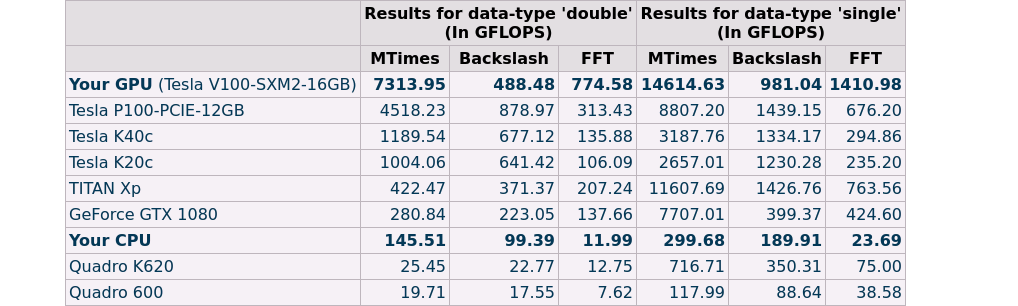
\includegraphics[width=\linewidth]{benchmark1.png}
	\caption{MATLAB Deep Learning Container on NVIDIA GPU Cloud Benchmark Overview.}
\end{figure}
\begin{figure}[H]
	\centering
	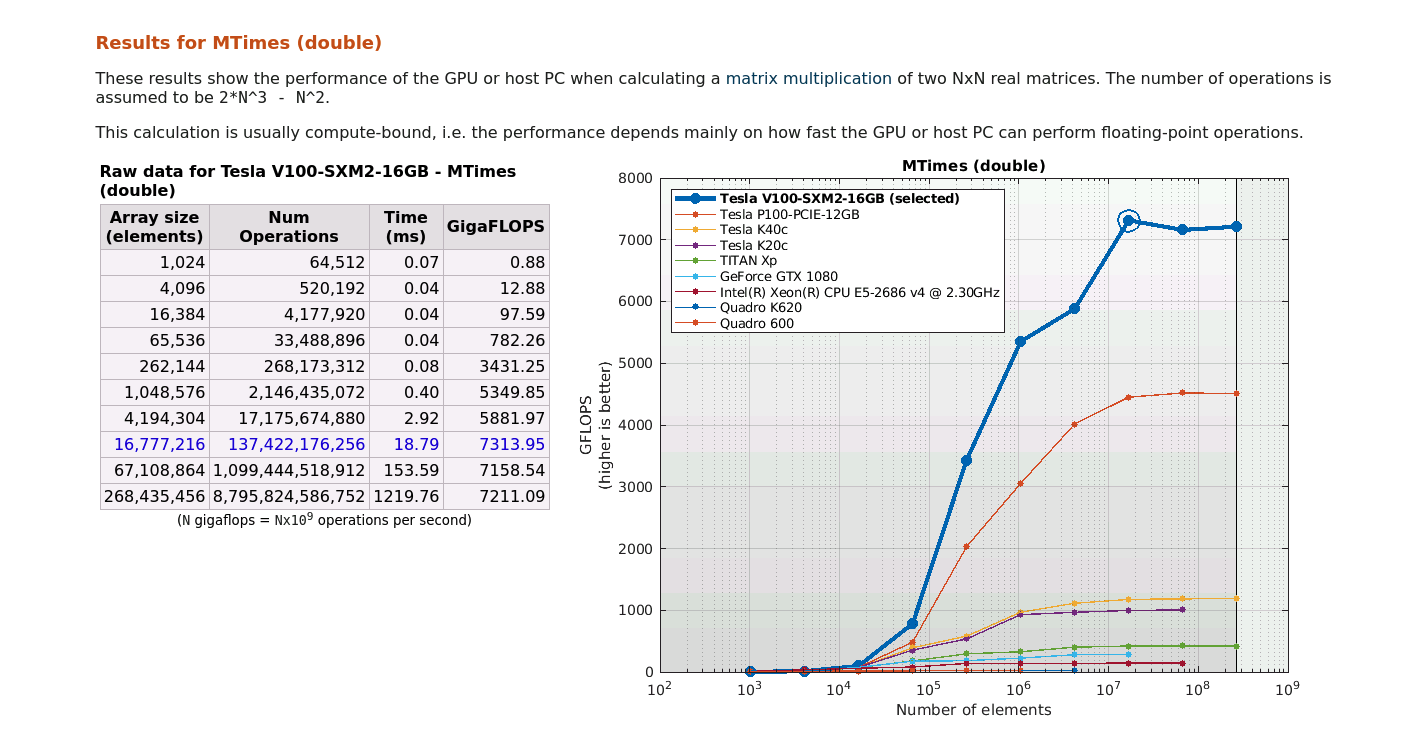
\includegraphics[width=\linewidth]{benchmark2.png}
	\caption{MATLAB Deep Learning Container on NVIDIA GPU Cloud Benchmark MTimes (double).}
\end{figure}
\begin{figure}[H]
	\centering
	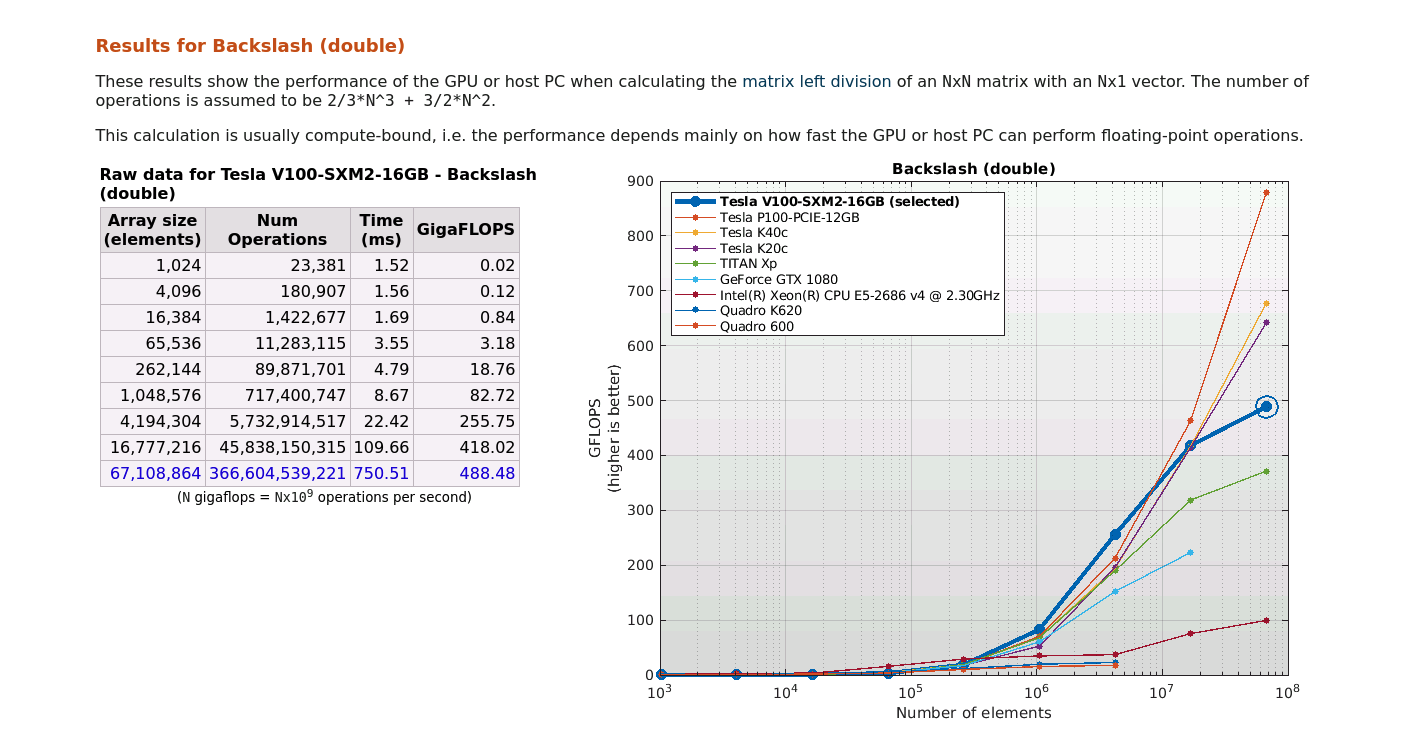
\includegraphics[width=\linewidth]{benchmark3.png}
	\caption{MATLAB Deep Learning Container on NVIDIA GPU Cloud Benchmark Backslash (double).}
\end{figure}
\begin{figure}[H]
	\centering
	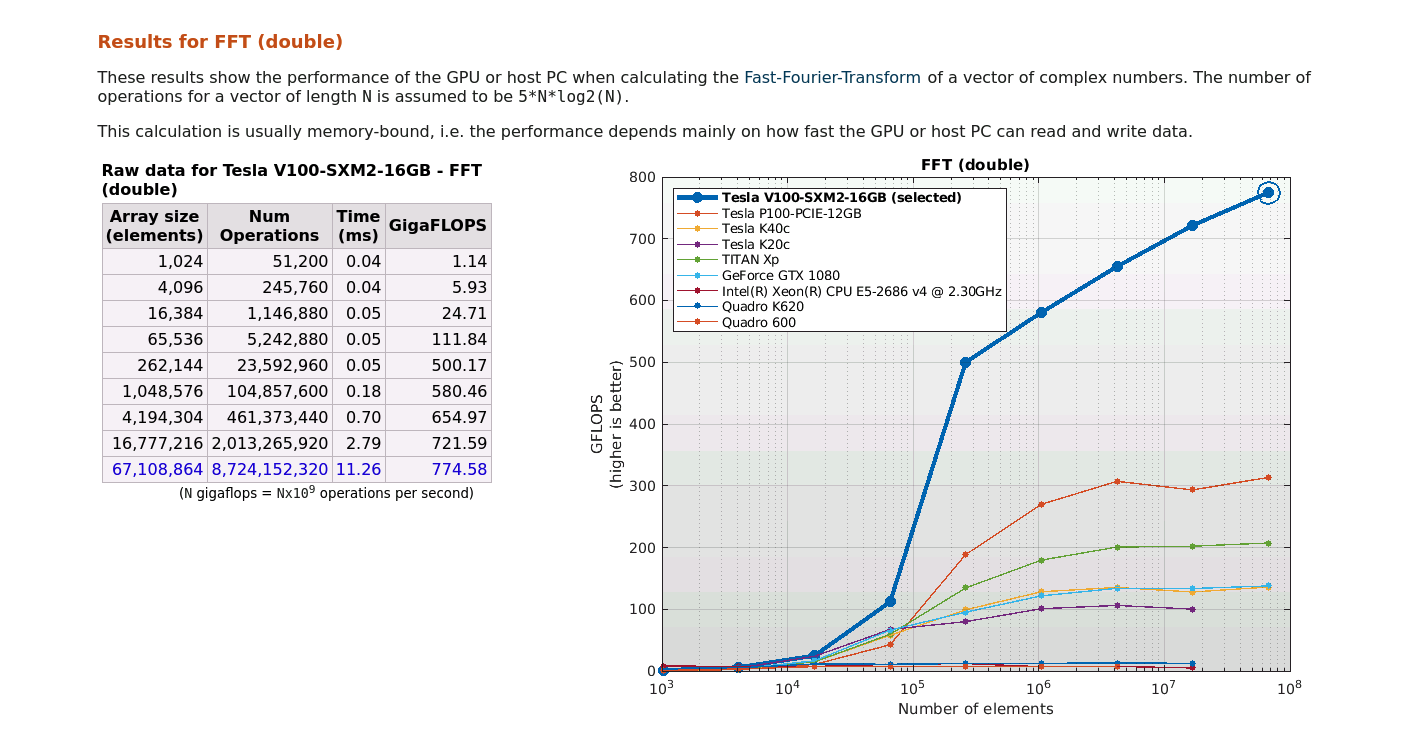
\includegraphics[width=\linewidth]{benchmark4.png}
	\caption{MATLAB Deep Learning Container on NVIDIA GPU Cloud Benchmark FFT (double).}
\end{figure}
\begin{figure}[H]
	\centering
	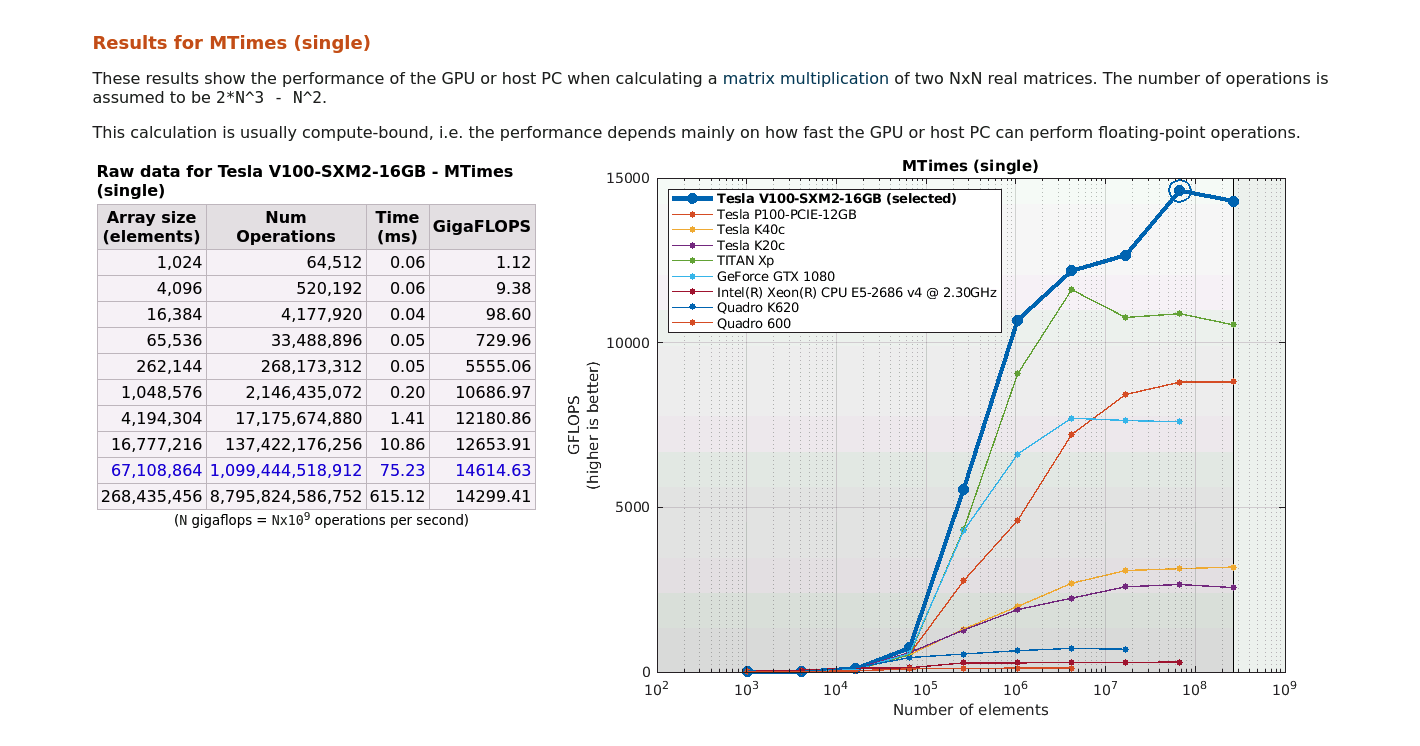
\includegraphics[width=\linewidth]{benchmark5.png}
	\caption{MATLAB Deep Learning Container on NVIDIA GPU Cloud Benchmark MTimes (single).}
\end{figure}
\begin{figure}[H]
	\centering
	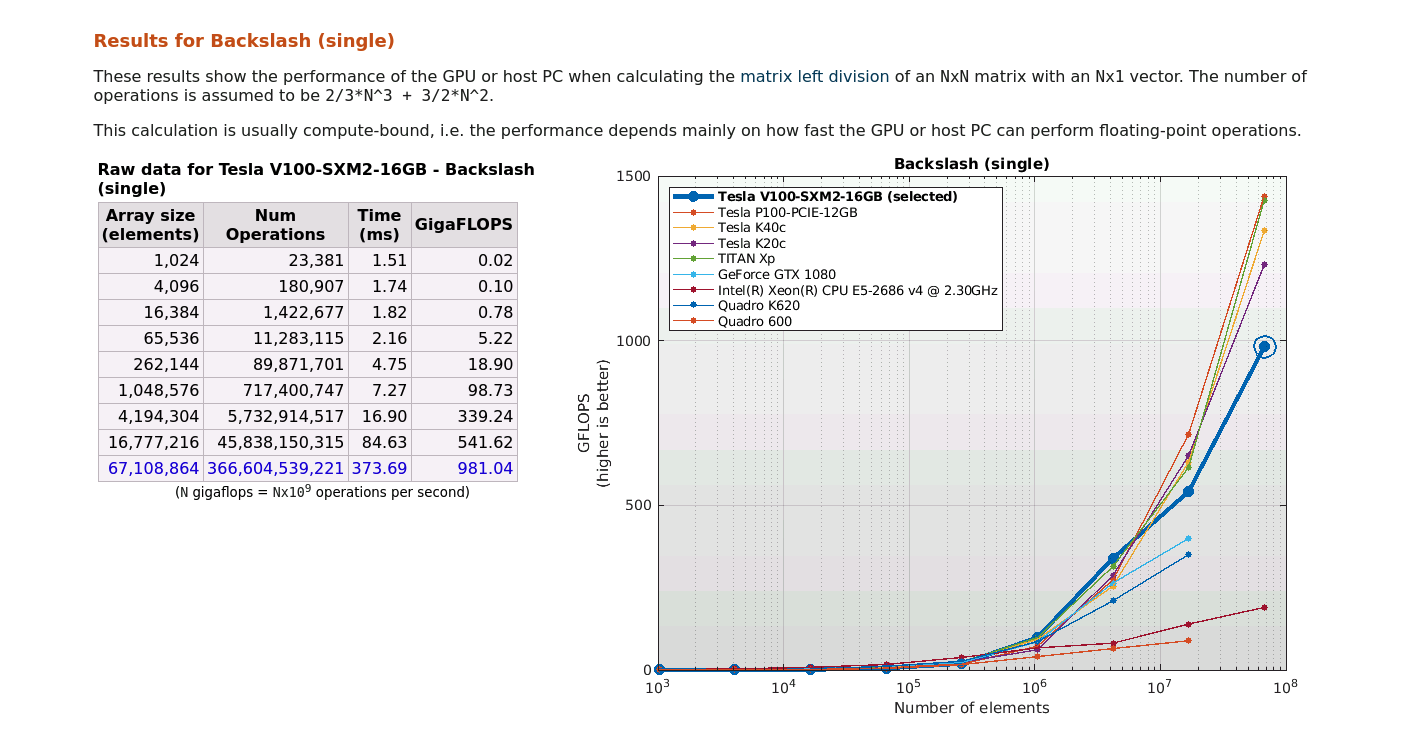
\includegraphics[width=\linewidth]{benchmark7.png}
	\caption{MATLAB Deep Learning Container on NVIDIA GPU Cloud Benchmark Backslash (single).}
\end{figure}
\begin{figure}[H]
	\centering
	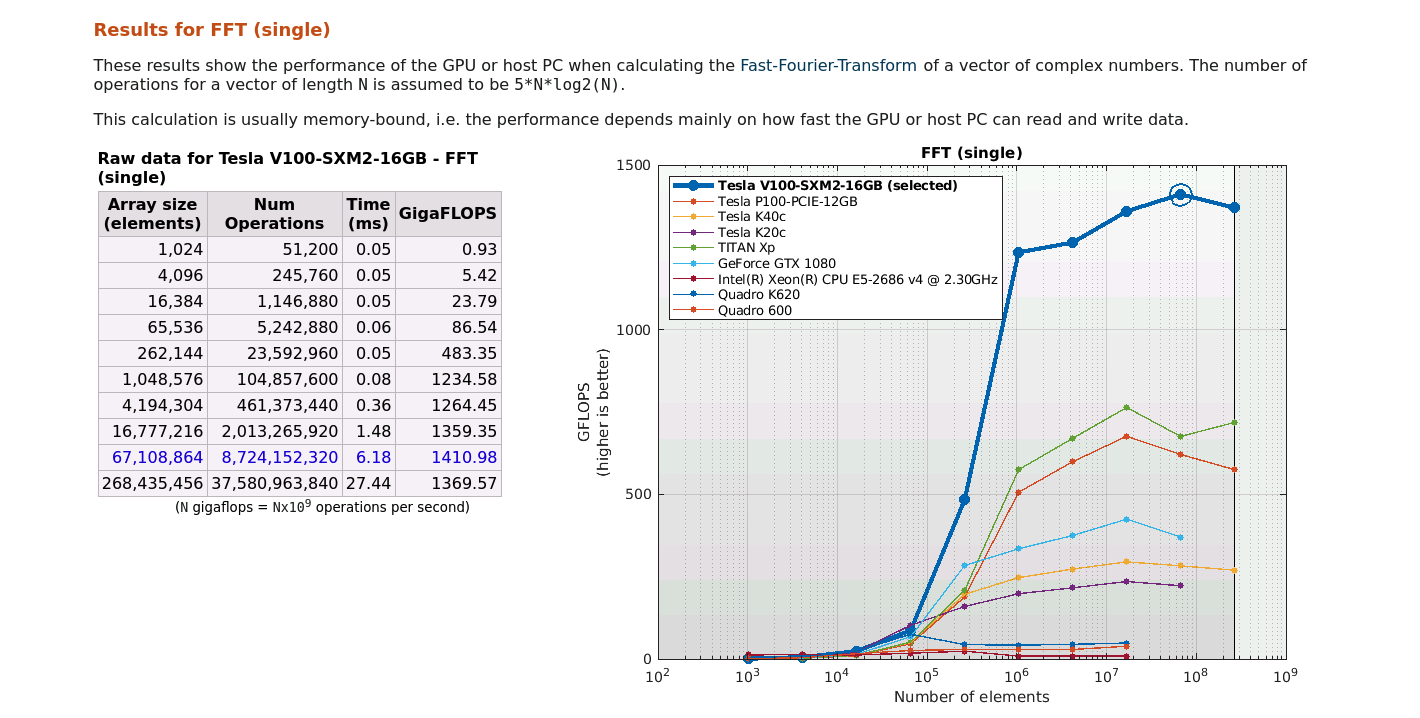
\includegraphics[width=\linewidth]{benchmark8.png}
	\caption{MATLAB Deep Learning Container on NVIDIA GPU Cloud Benchmark FFT (single).}
\end{figure}
\begin{figure}[H]
	\centering
	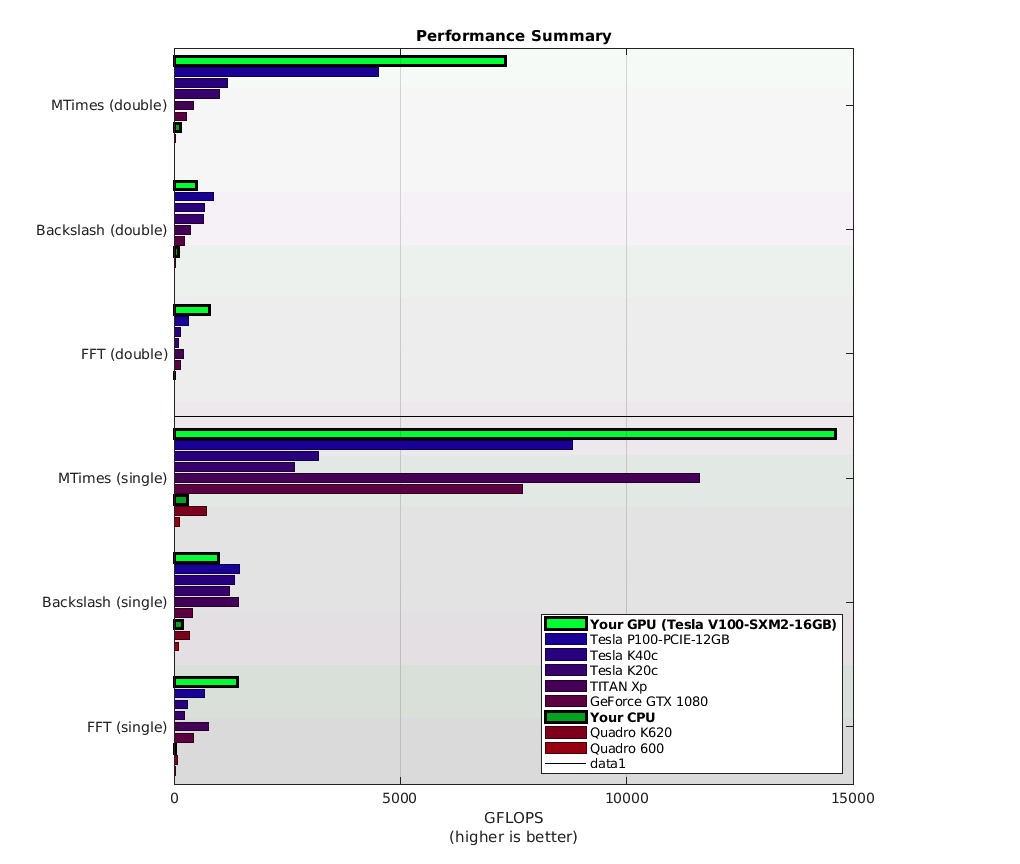
\includegraphics[width=0.8\linewidth]{benchmark9.png}
	\caption{MATLAB Deep Learning Container on NVIDIA GPU Cloud Benchmark Overview Diagram.}
\end{figure}
\chapter{GPU computing in Matlab}
\section{Basic GPU usage}
The functions 'gpuArray()' and 'gather()':
\begin{algorithm}
	\fbox{\begin{minipage}{\linewidth}
		$>>$A = gpuArray(B) \% Matrix B is copied to the GPU dedicated memory, giving it name A.\\
		$>>$B = gather(A)   \% Matrix A is copied to the CPU memory, giving it name B.\\
	\end{minipage}}
\end{algorithm}
Functions to create special kind of matrices can be used with the tag 'gpuArray' to directly create them on the GPU dedicated memory.
Special matrix create function are: ones(), zeros(), rand(),eye(),...
\begin{algorithm}
	\fbox{\begin{minipage}{\linewidth}
			$>>$A = ones(10,5,'gpuArray')  \\
			$>>$A = eye(10,5,'gpuArray') \% eye() creates an identity matrix.\\
			$>>$clear A; to free up when matrix A is no longer needed in GPU dedicated memory.\\
	\end{minipage}}
\end{algorithm}

% Back cover: change according to the correct campus
%
\includepdf{private/back_fiiw_denayer.pdf}
% 
\includepdf{private/back_fiiw_denayer_eng.pdf} % For the english version
%
\includepdf{private/back_fiiw_geel.pdf}
% 
\includepdf{private/back_fiiw_geel_eng.pdf} % For the english version

\includepdf{private/back_fiiw_gent.pdf}
%
\includepdf{private/back_fiiw_ghent_eng.pdf} % For the english version
%
\includepdf{private/back_fiiw_brugge.pdf}
% 
\includepdf{private/back_fiiw_bruges_eng.pdf} % For the english version
%
\includepdf{private/back_fiiw_groept.pdf}
% \includepdf{private/back_fiiw_groupt_eng.pdf} % For the english version

\end{document}
